%\documentclass[a4,semhelv,landscape]{seminar}
\documentclass[landscape]{slides}
%\documentclass[pdf, default, slideBW, nocolorBG]{prosper}
\usepackage[left=0.2cm,top=0.2cm,right=0.2cm,bottom=0.2cm,nohead,nofoot]{geometry}
%\def\everyslide{\sffamily}
%\usepackage{fullpage}
\usepackage{graphicx}
\usepackage[usenames]{color}
%\usepackage{color}
\usepackage{verbatim}
\usepackage{nopageno}
\usepackage{setspace}
%\usepackage{times}
% define some nice colors
\definecolor{myred}{rgb}{0.6,0,0}
\definecolor{myblue}{rgb}{0,0.2,0.4}
\definecolor{mygreen}{rgb}{0,0.5,0.0}
\definecolor{mypurple}{cmyk}{0.5,1.0,0.0,0.0}
%\color{myblue}

\begin{document}
%%%%%%%%%%%%%%%%%%%%%%%%%%%%%%%%%%%%%%%%%%%%%%%%%%%%%%%%%%%%%%%%%%%%
%Slide 0 - title
\begin{slide}
\begin{center}
\large{\textbf{Structural RNA and viral sequence analysis}}

\normalsize

Eric Nawrocki \\

\medskip

\medskip

\medskip

\medskip

\medskip

\small
\begin{tabular}{c}
%Alejandro Sch\"{a}ffer's group \\
%\\
Intramural Research Program\\
National Library of Medicine\\
National Institutes of Health\\
\\
%Howard Hughes Medical Institute \\ 
%Janelia Research Campus \\
\end{tabular}

\vspace{0.1in}


\includegraphics[width=2.5in]{figs/NIH_NLM_ABRV_2C_4-white}
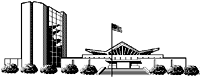
\includegraphics[width=2.5in]{figs/nlm-buildings}

\end{center}
\end{slide}

%%%%%%%%%%%%%%%%%%%%%%%%%%%%%%%%%%%%%%%%%%%%%%%%%%%%%%%%%%%%%%%%%%%%
\begin{slide}
\begin{center}
\Large
  \textbf{Two main areas of my research:}

\begin{description}
\item[1.] Viral sequence analysis tools, since 2015
\item[2.] Structural RNA analysis tools, since 2004
\end{description}

\end{center}
\vfill
\end{slide}
%%%%%%%%%%%%%%%%%%%%%%%%%%%%%%%%%%%%%%%%%%%%%%%%%%%%%%%%%%%%%%%%%%%%
\begin{slide}
\begin{center}
\large{\textbf{GenBank indexers handle incoming sequence submissions}}
\end{center}

\center{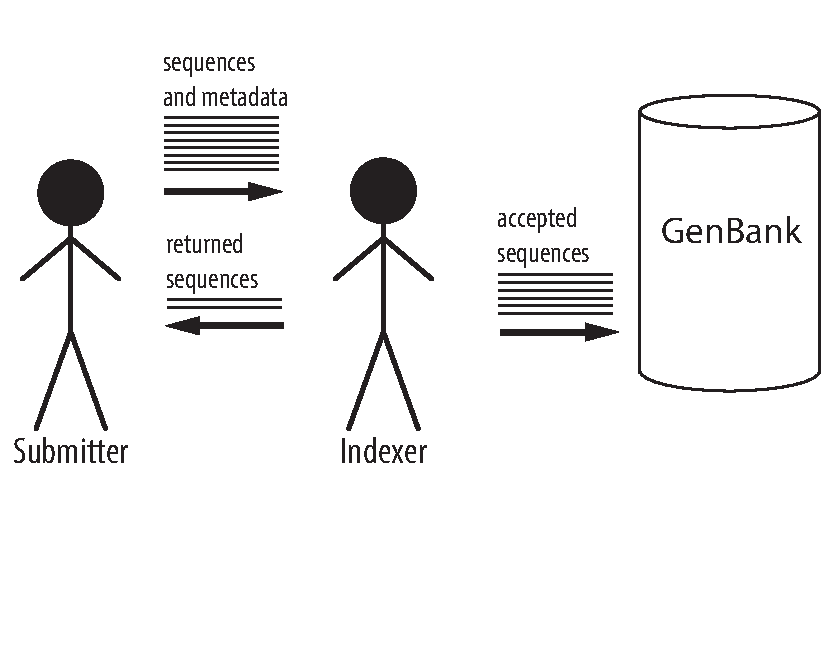
\includegraphics[width=9in]{figs/spheres-submission-schematic-1}}

\vfill
\end{slide}
%%%%%%%%%%%%%%%%%%%%%%%%%%%%%%%%%%%%%%%%%%%%%%%%%%%%%%%%%%%%%%%%%%%%%%
\begin{slide}
\begin{center}

\includegraphics[width=10in]{figs/vadr-title-paper}

\begin{itemize}
\item general tool for reference-based annotation of viral sequences
\item used for Norovirus and Dengue virus submissions since 2018
\item used for SARS-CoV-2 submissions since March 2020 
\item also used manually for RSV, Mpox, and some Influenza submissions
\end{itemize}

\vfill
\end{center}
\end{slide}
%%%%%%%%%%%%%%%%%%%%%%%%%%%%%%%%%%%%%%%%%%%%%%%%%%%%%%%%%%%%%%%%%%%%%%
\begin{slide}
\begin{center}
\large{\textbf{VADR assists GenBank indexers: \\ Each sequence \textcolor{green}{PASSes} or \textcolor{red}{FAILs}}}
\end{center}

\center{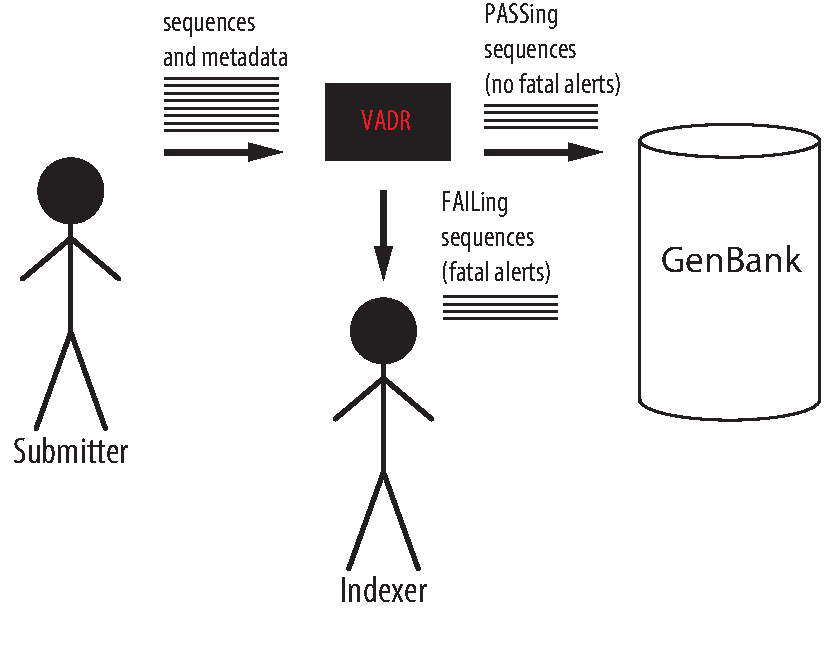
\includegraphics[width=9in]{figs/spheres-submission-schematic-2}}

\vfill
\end{slide}
%%%%%%%%%%%%%%%%%%%%%%%%%%%%%%%%%%%%%%%%%%%%%%%%%%%%%%%%%%%%%%%%%%%%%%
\begin{slide}
\begin{center}
\textbf{Indexers decide fate of some \textcolor{red}{FAILing} sequences\\ but some are sent directly back to submitter with error reports}
\end{center}

%\center{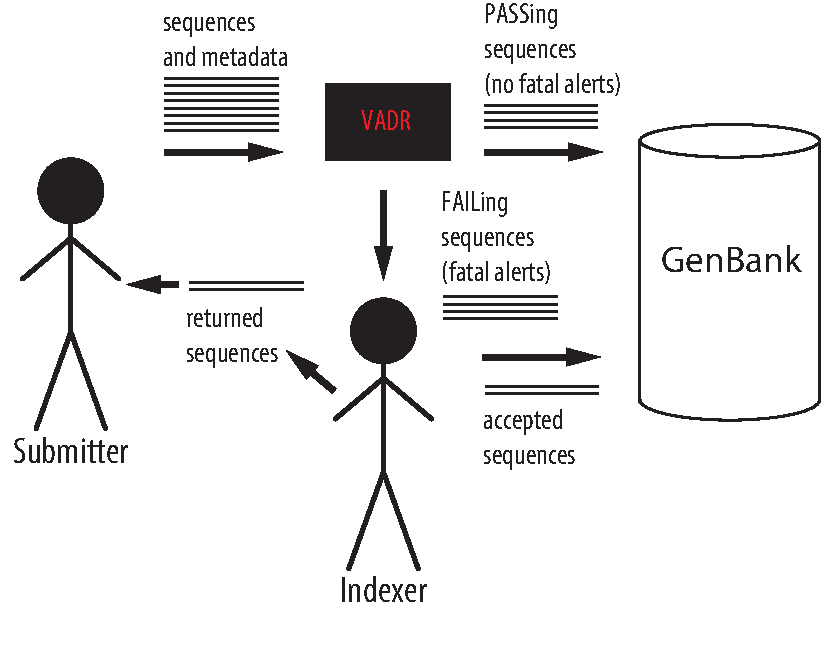
\includegraphics[width=9in]{figs/spheres-submission-schematic-3}}
\center{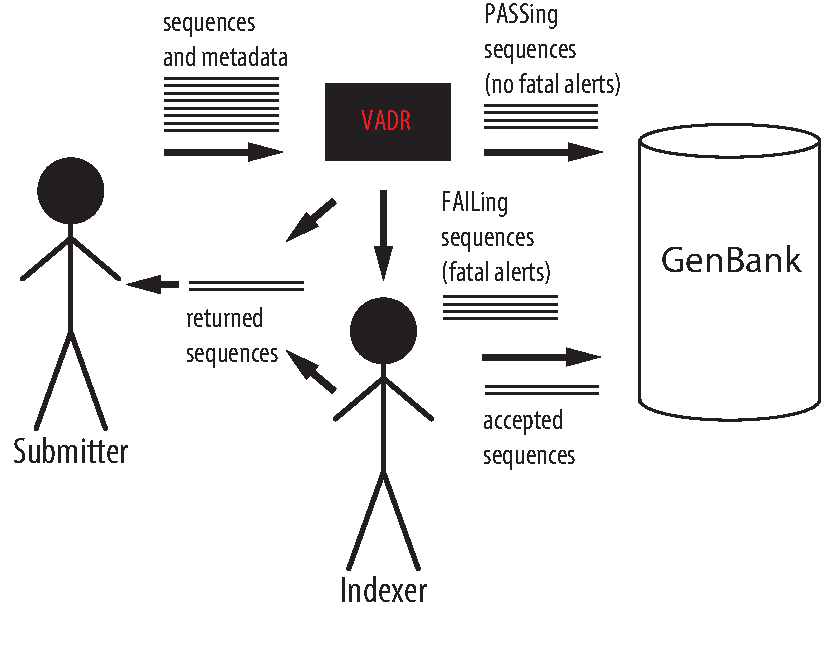
\includegraphics[width=9in]{figs/spheres-submission-schematic-4}}

\vfill
\end{slide}
%%%%%%%%%%%%%%%%%%%%%%%%%%%%%%%%%%%%%%%%%%%%%%%%%%%%%%%%%%%%%%%%%%%%%%
\begin{slide}
\begin{center}
\large{\textbf{VADR builds a reference model of a \\ RefSeq and its features}}
\end{center}

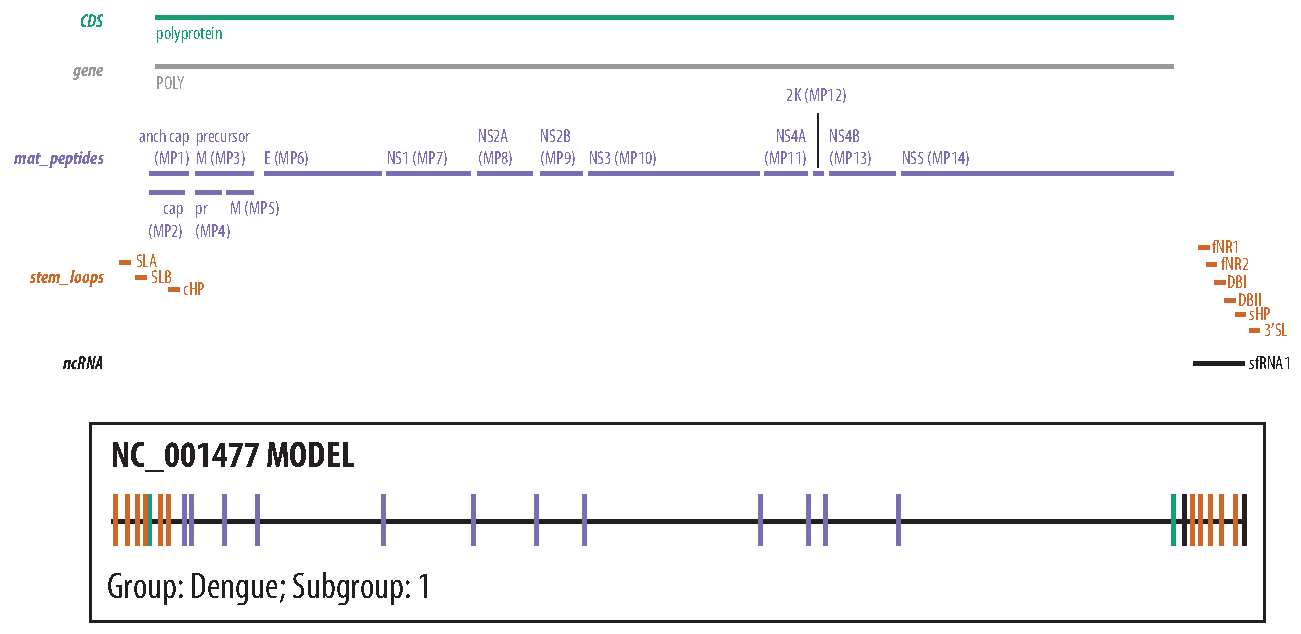
\includegraphics[width=10.5in]{figs/dengue-features}

\vfill
\end{slide}
%%%%%%%%%%%%%%%%%%%%%%%%%%%%%%%%%%%%%%%%%%%%%%%%%%%%%%%%%%%%%%%%%%%%%%
\begin{slide}
\begin{center}
%\textbf{\texttt{v-annotate.pl} annotates each sequence using its
\large{\textbf{VADR validates and annotates each input sequence \\ using its 
  best-matching model}}

\begin{itemize}
\item Each sequence $S$ proceeds through 4 stages:
%\item For each sequence $S$:
\small
\begin{enumerate}
%\item \textbf{Classification}: compare $S$ to all models to find best matching model $M$
\item \textbf{Classification}
%\item \textbf{Coverage determination}: search $M$ against $S$ to find 'hits'
\item \textbf{Coverage determination}
%\item \textbf{Alignment}: align $S$ to $M$ and map features from $M$ to $S$
\item \textbf{Alignment}
%\item \textbf{Protein validation}: compare predicted CDS in $S$ to proteins
\item \textbf{Protein validation}
\end{enumerate}
\end{itemize}

\normalsize
\emph{Different types of alerts are identified and reported at each stage}

\end{center}

\vfill
\end{slide}
%%%%%%%%%%%%%%%%%%%%%%%%%%%%%%%%%%%%%%%%%%%%%%%%%%%%%%%%%%%%%%%%%%%%%%
\begin{slide}
\begin{center}

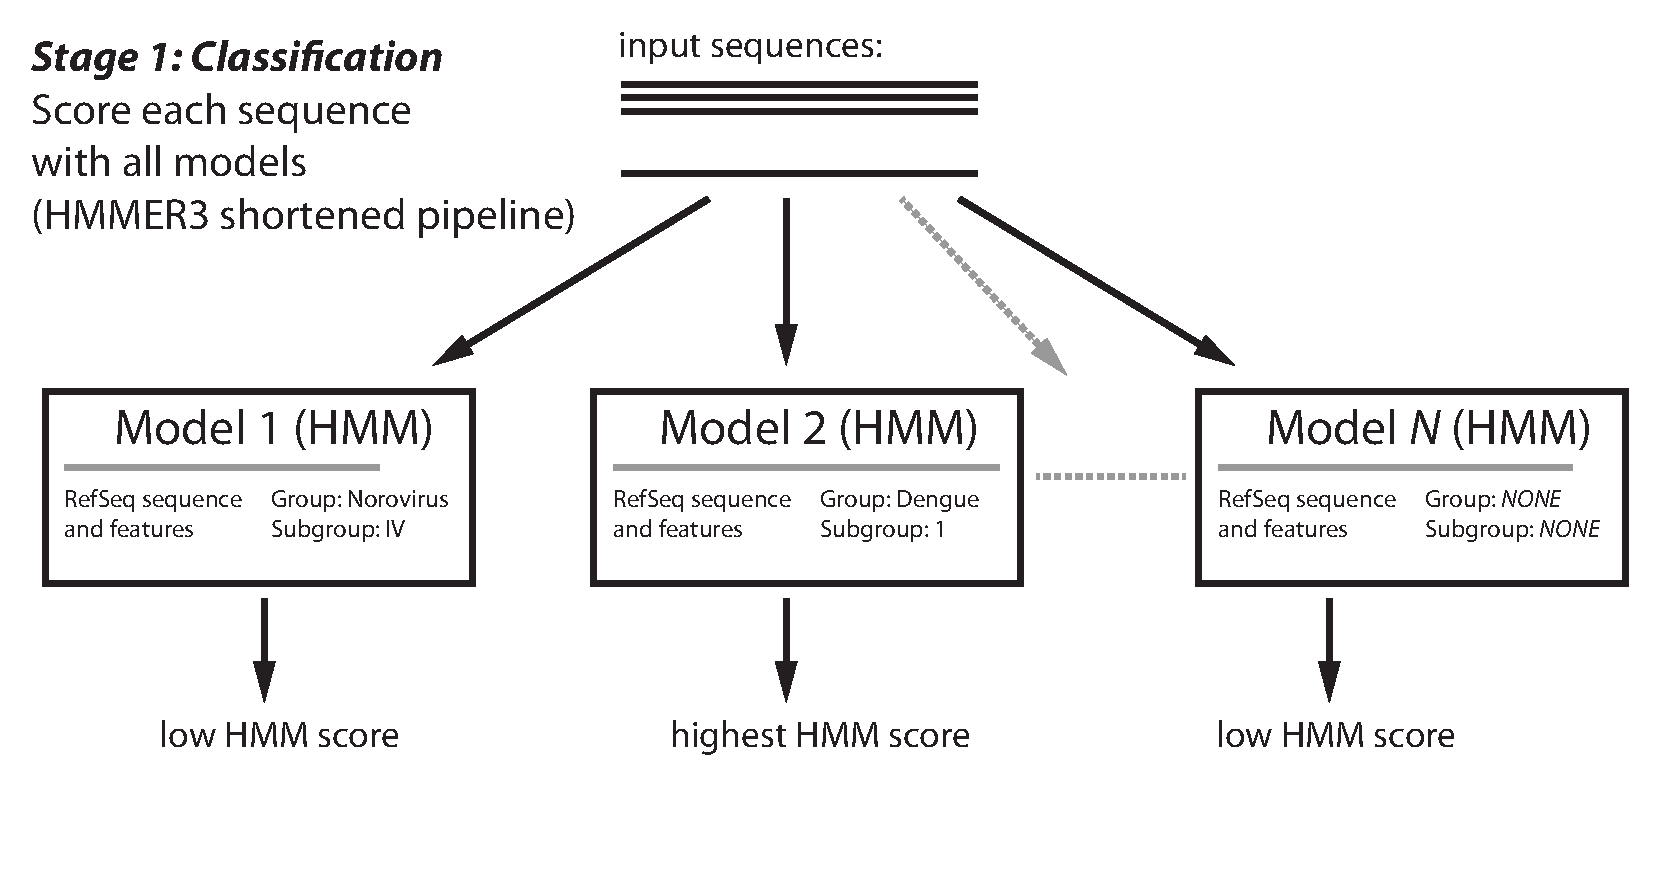
\includegraphics[width=9.5in]{figs/v-annotate-stage1-1}

\end{center}
\vfill
\end{slide}
%%%%%%%%%%%%%%%%%%%%%%%%%%%%%%%%%%%%%%%%%%%%%%%%%%%%%%%%%%%%%%%%%%%%%%
\begin{slide}
\begin{center}

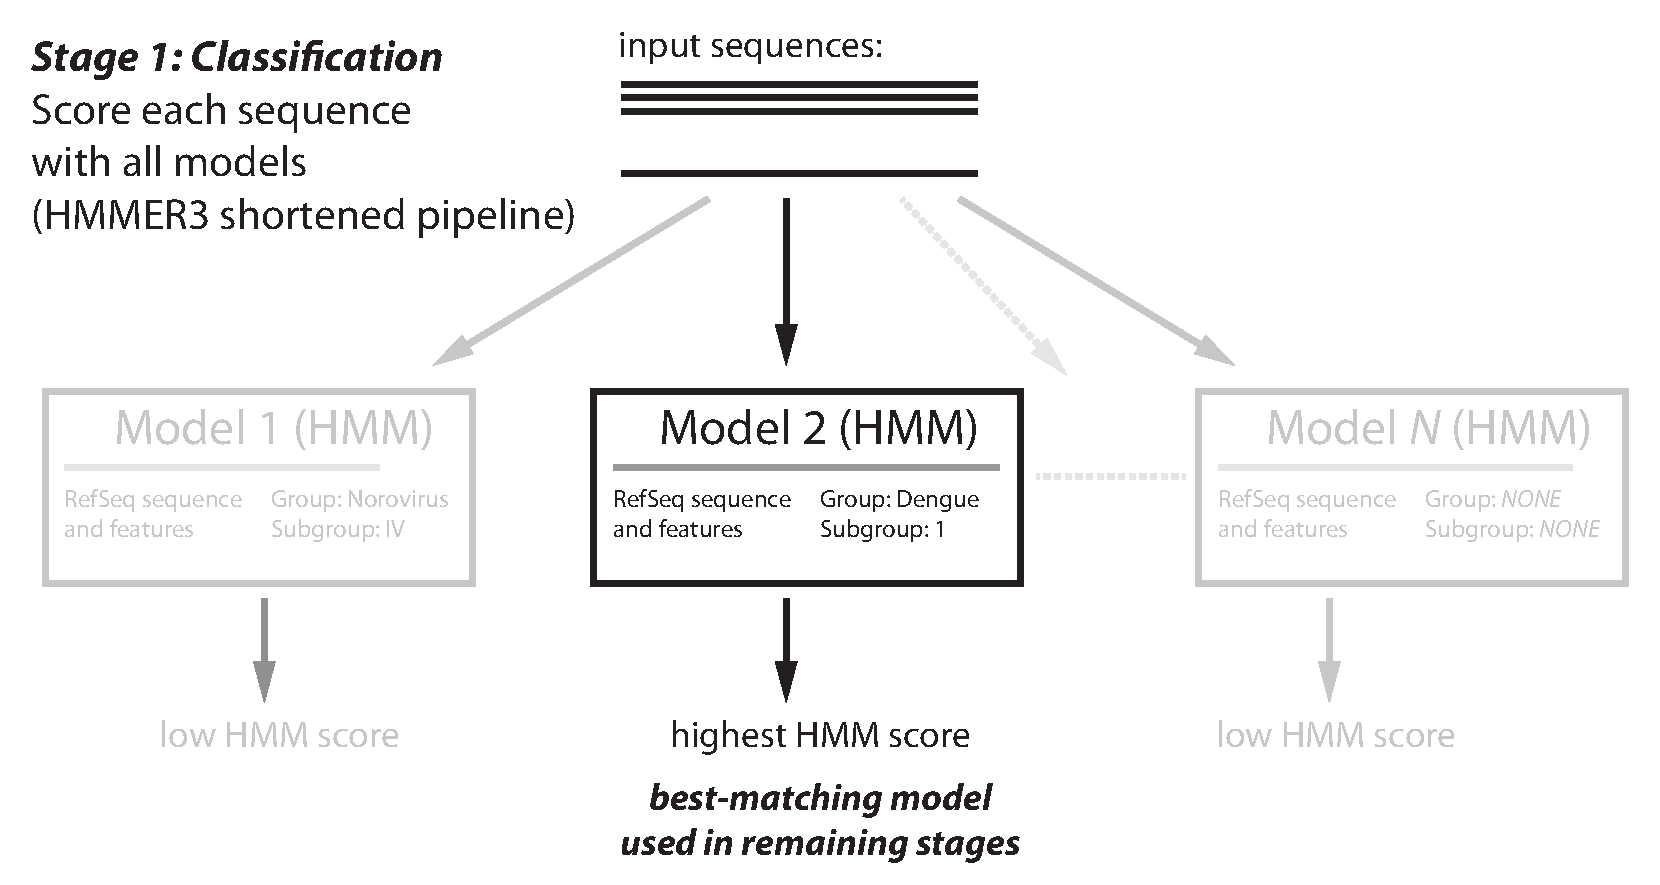
\includegraphics[width=9.5in]{figs/v-annotate-stage1-2}

\end{center}
\vfill
\end{slide}
%%%%%%%%%%%%%%%%%%%%%%%%%%%%%%%%%%%%%%%%%%%%%%%%%%%%%%%%%%%%%%%%%%%%%%
\begin{slide}
\begin{center}

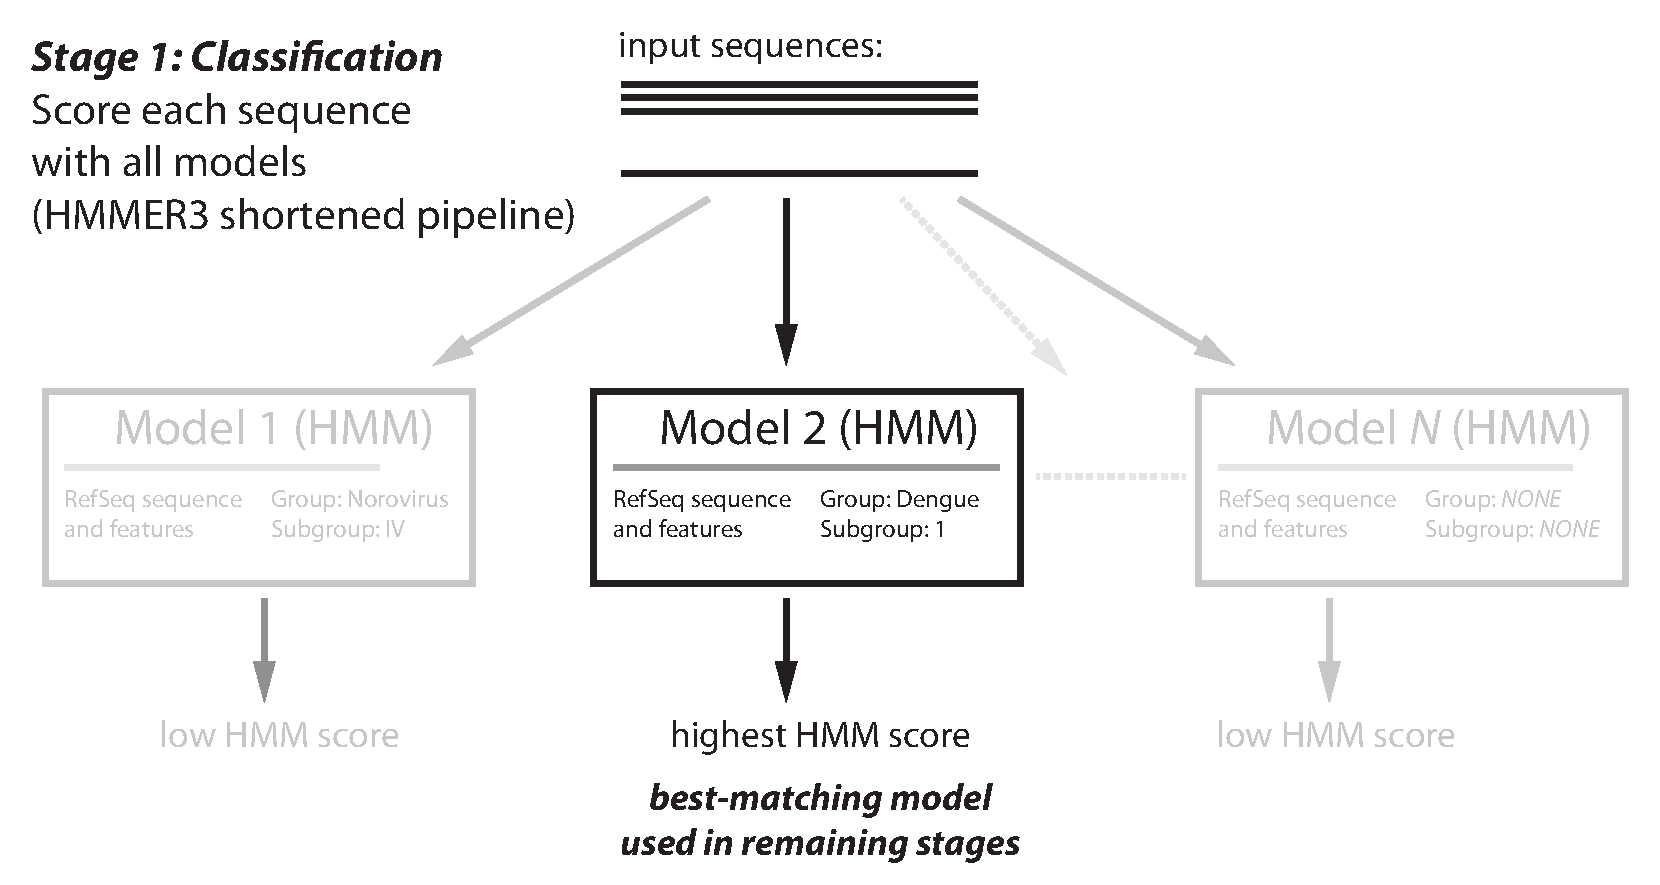
\includegraphics[width=9.5in]{figs/v-annotate-stage1-2}

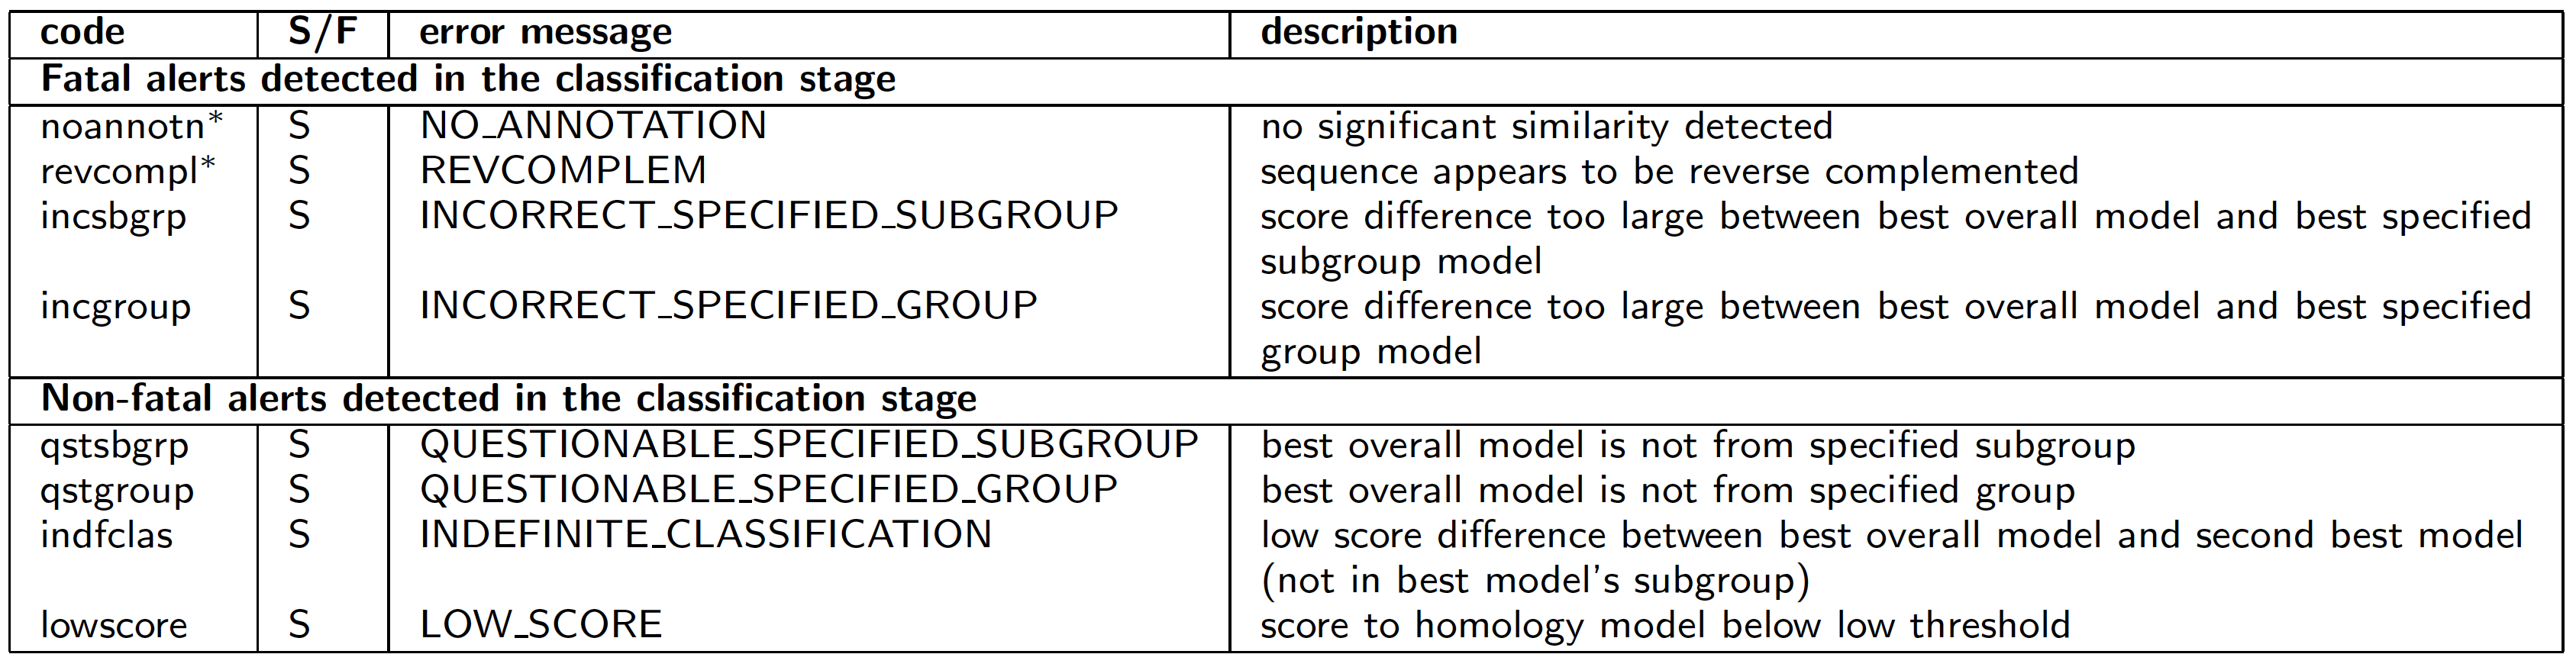
\includegraphics[width=10.5in]{figs/ss-class-alert-list}

\end{center}
\vfill
\end{slide}
%%%%%%%%%%%%%%%%%%%%%%%%%%%%%%%%%%%%%%%%%%%%%%%%%%%%%%%%%%%%%%%%%%%%%%
\begin{slide}
\begin{center}

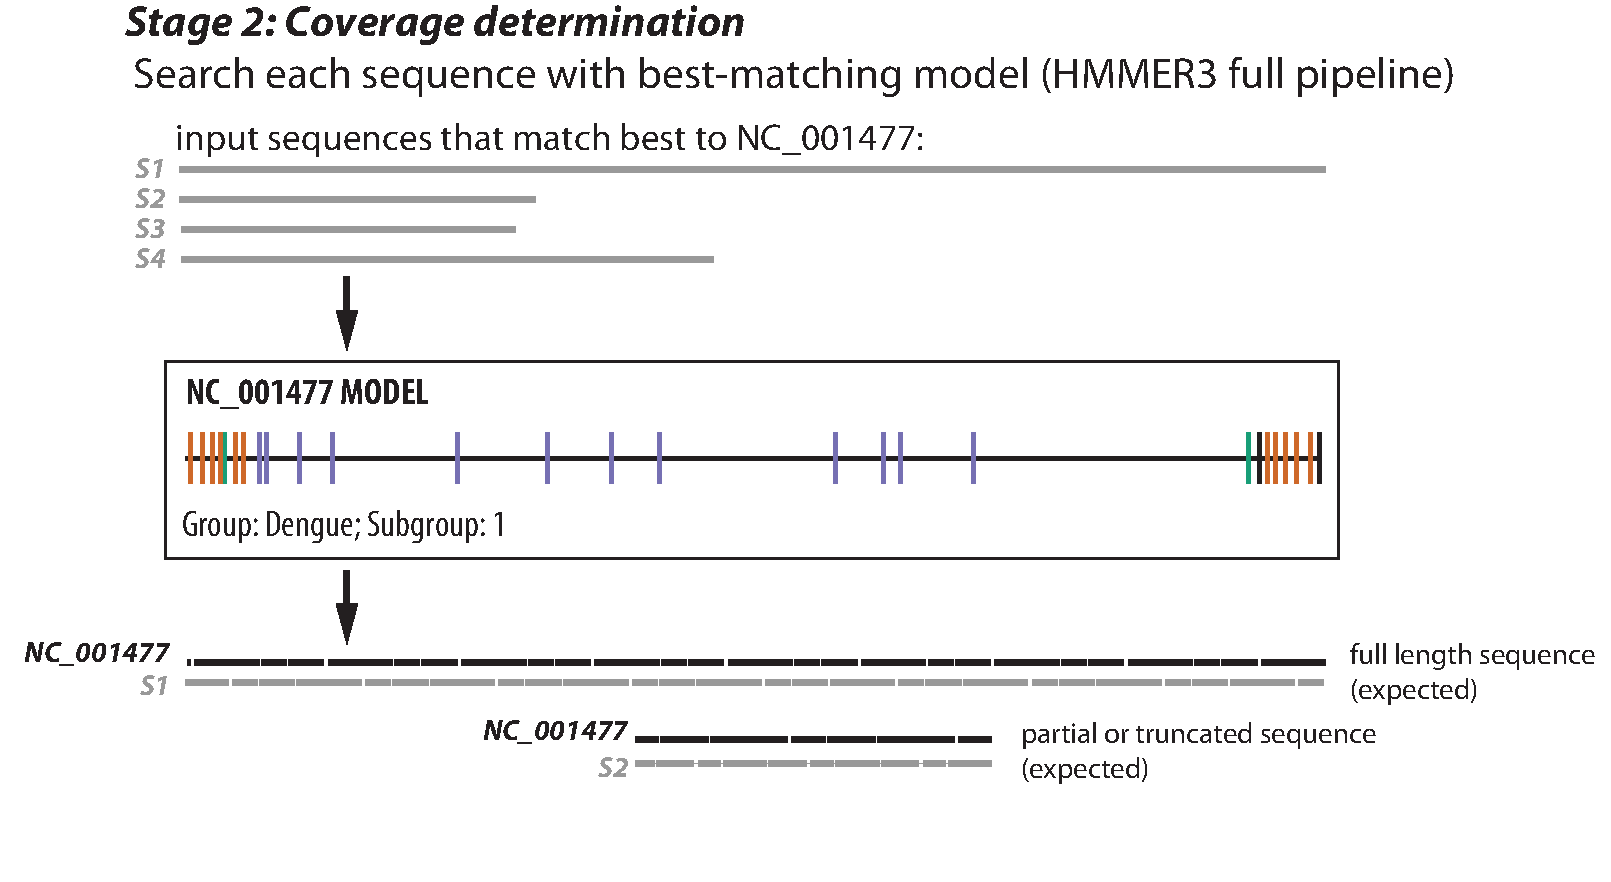
\includegraphics[width=10.5in]{figs/v-annotate-stage2-1}

\end{center}
\vfill
\end{slide}
%%%%%%%%%%%%%%%%%%%%%%%%%%%%%%%%%%%%%%%%%%%%%%%%%%%%%%%%%%%%%%%%%%%%%%
\begin{slide}
\begin{center}

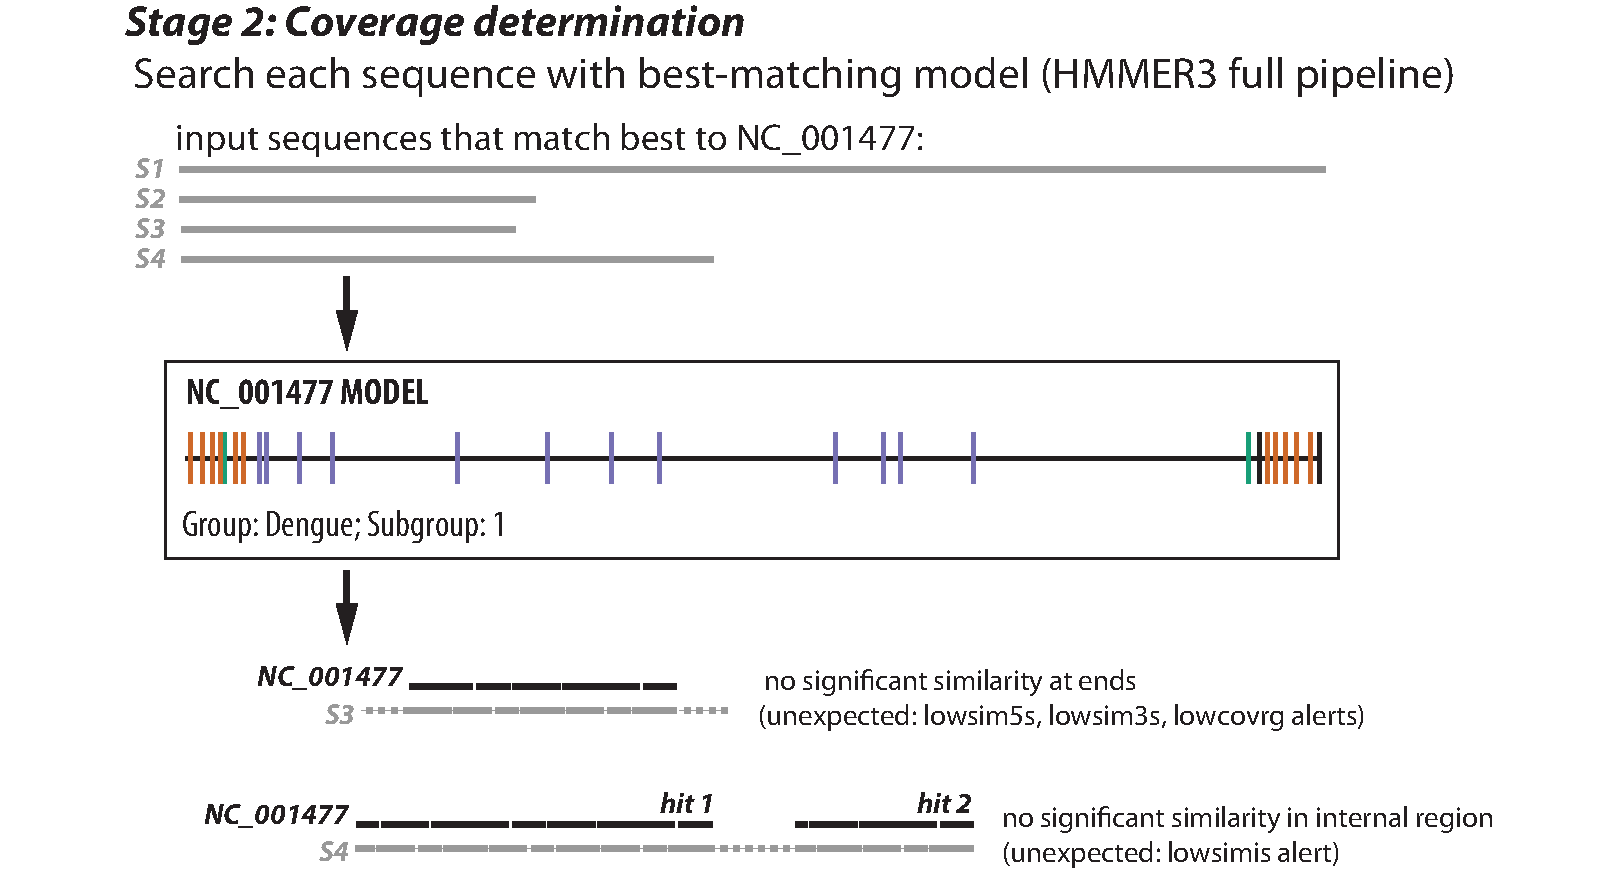
\includegraphics[width=10.5in]{figs/v-annotate-stage2-2}
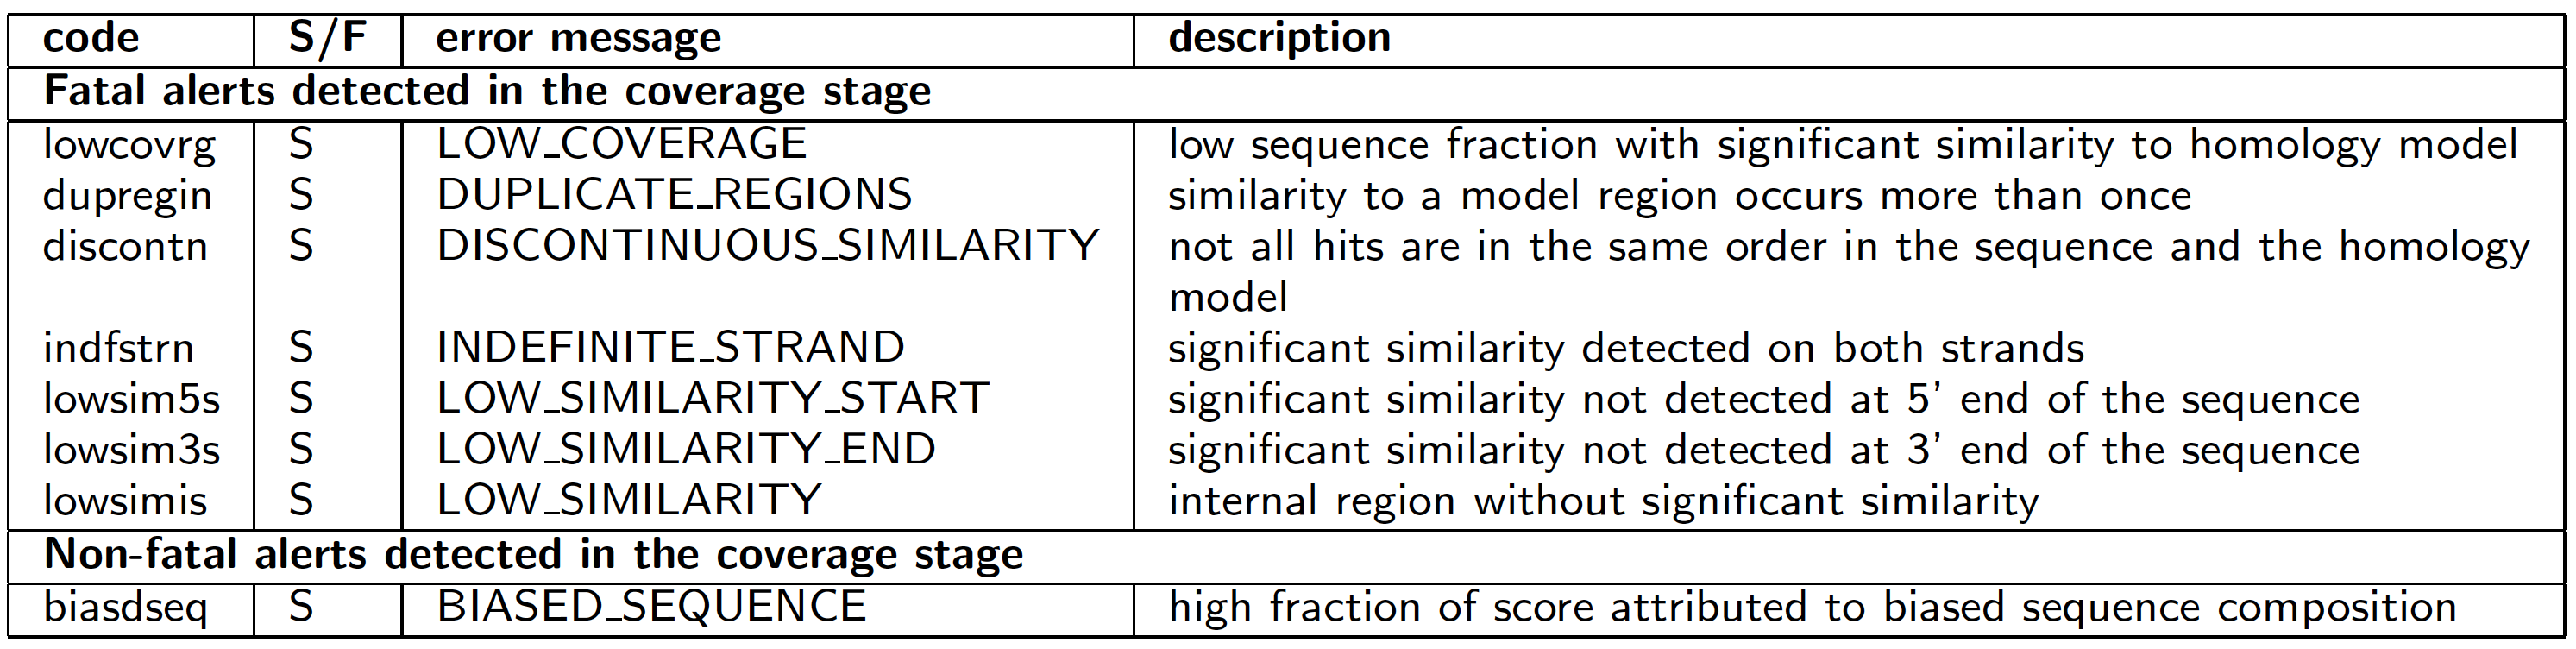
\includegraphics[width=10in]{figs/ss-coverage-alert-list}
\end{center}

\vfill
\end{slide}
%%%%%%%%%%%%%%%%%%%%%%%%%%%%%%%%%%%%%%%%%%%%%%%%%%%%%%%%%%%%%%%%%%%%%%
\begin{slide}
\begin{center}

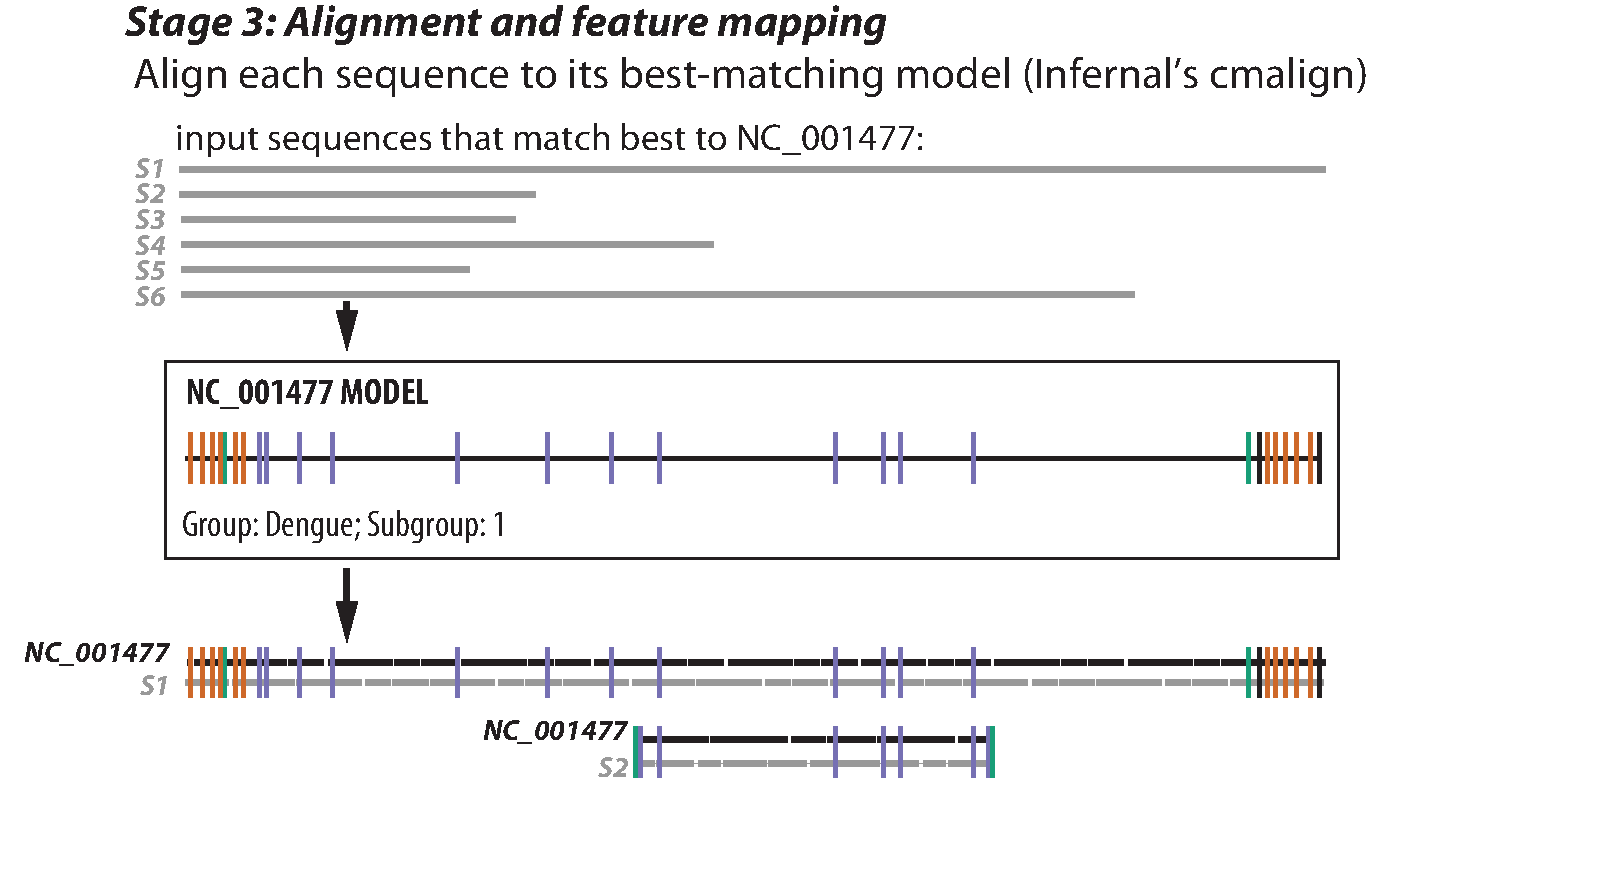
\includegraphics[width=10.5in]{figs/v-annotate-stage3-1}
\end{center}

\vfill
\end{slide}
%%%%%%%%%%%%%%%%%%%%%%%%%%%%%%%%%%%%%%%%%%%%%%%%%%%%%%%%%%%%%%%%%%%%%%
%\begin{slide}
%\begin{center}
%
%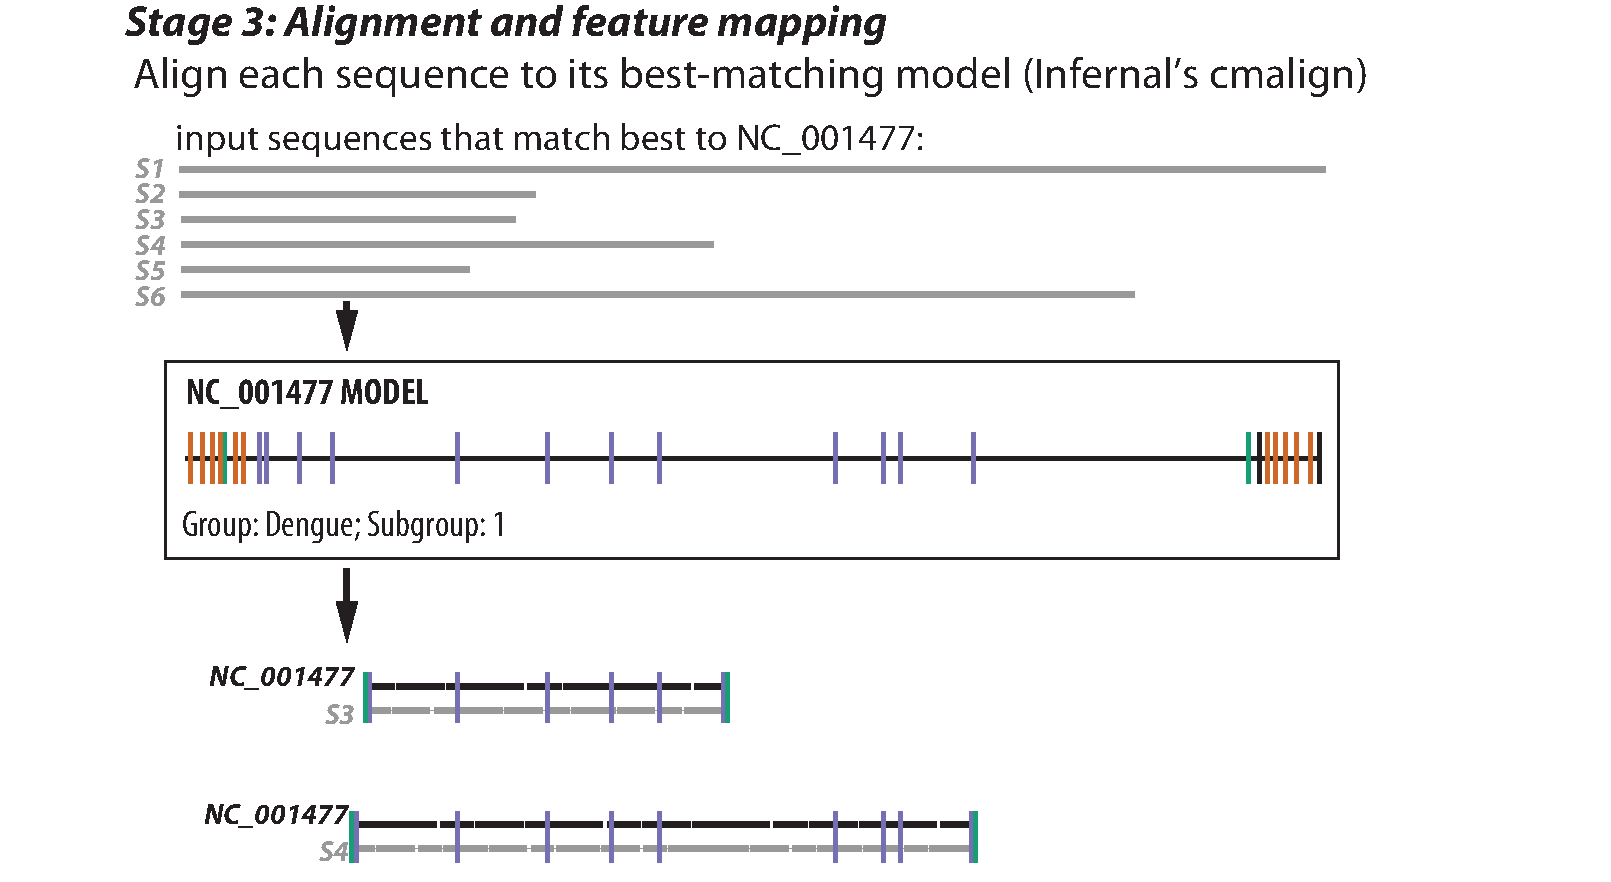
\includegraphics[width=10.5in]{figs/v-annotate-stage3-2}
%\end{center}
%
%\vfill
%\end{slide}
%%%%%%%%%%%%%%%%%%%%%%%%%%%%%%%%%%%%%%%%%%%%%%%%%%%%%%%%%%%%%%%%%%%%%%
%\begin{slide}
%\begin{center}
%
%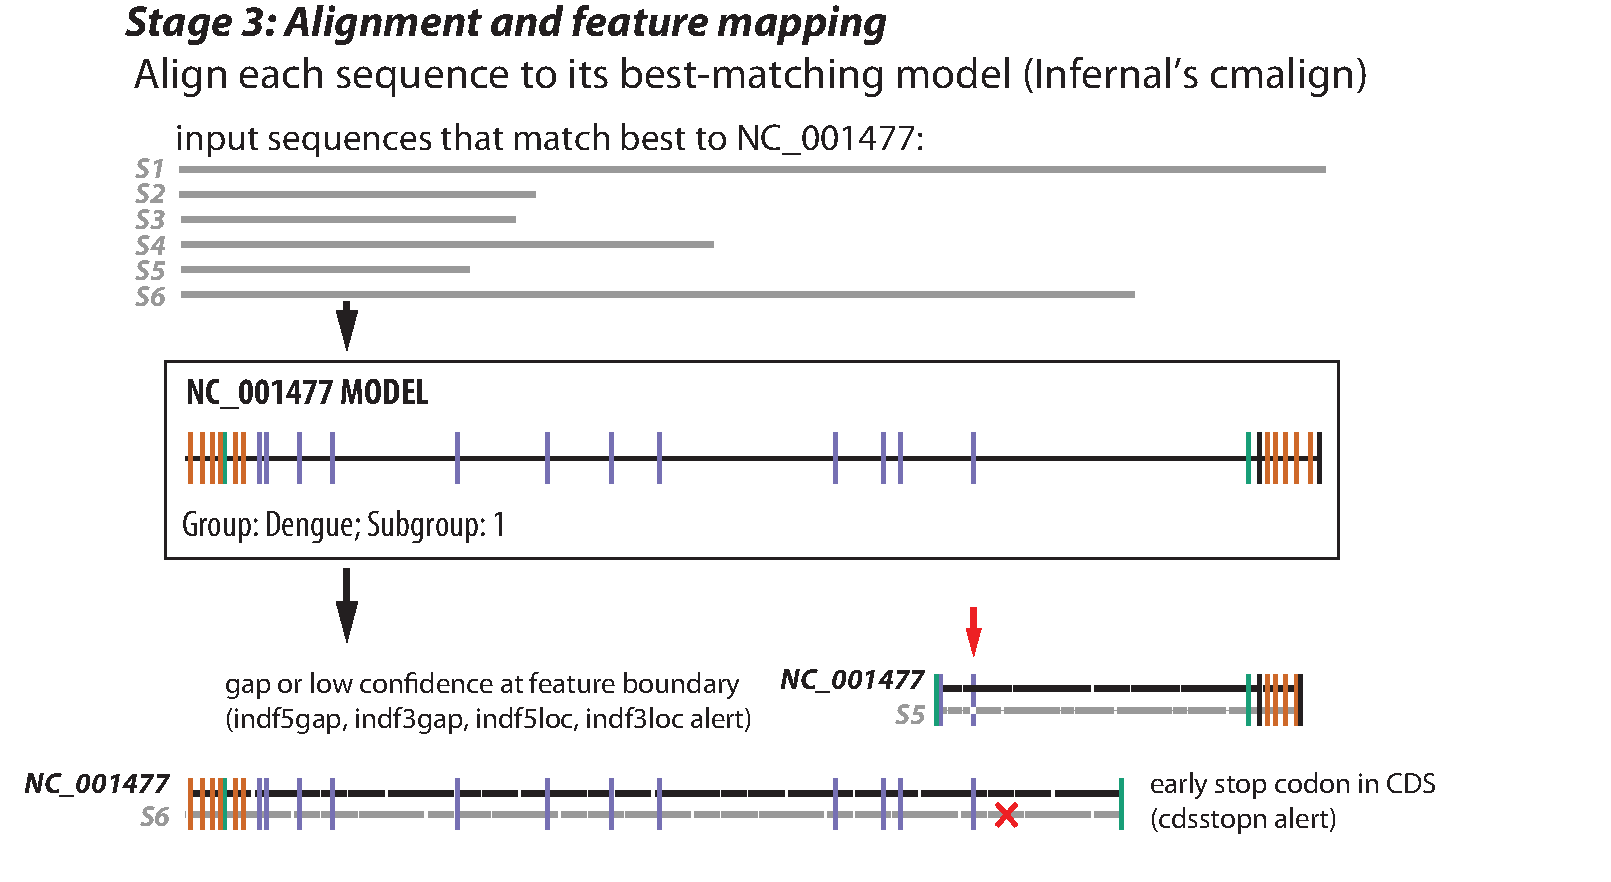
\includegraphics[width=10.5in]{figs/v-annotate-stage3-3}
%\end{center}
%
%\vfill
%\end{slide}
%%%%%%%%%%%%%%%%%%%%%%%%%%%%%%%%%%%%%%%%%%%%%%%%%%%%%%%%%%%%%%%%%%%%%%
\begin{slide}
\begin{center}

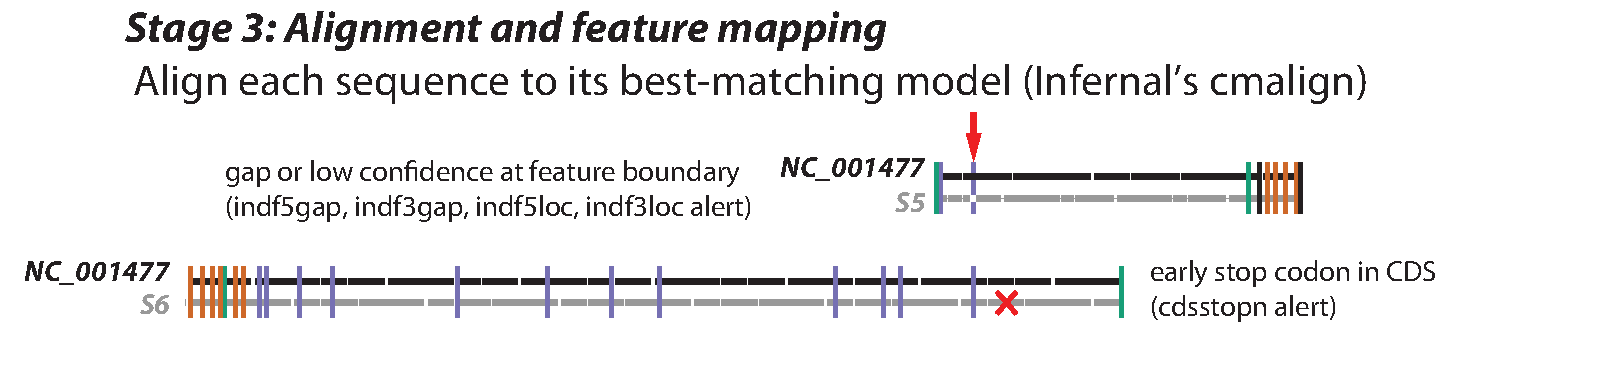
\includegraphics[width=10.5in]{figs/v-annotate-stage3-4}
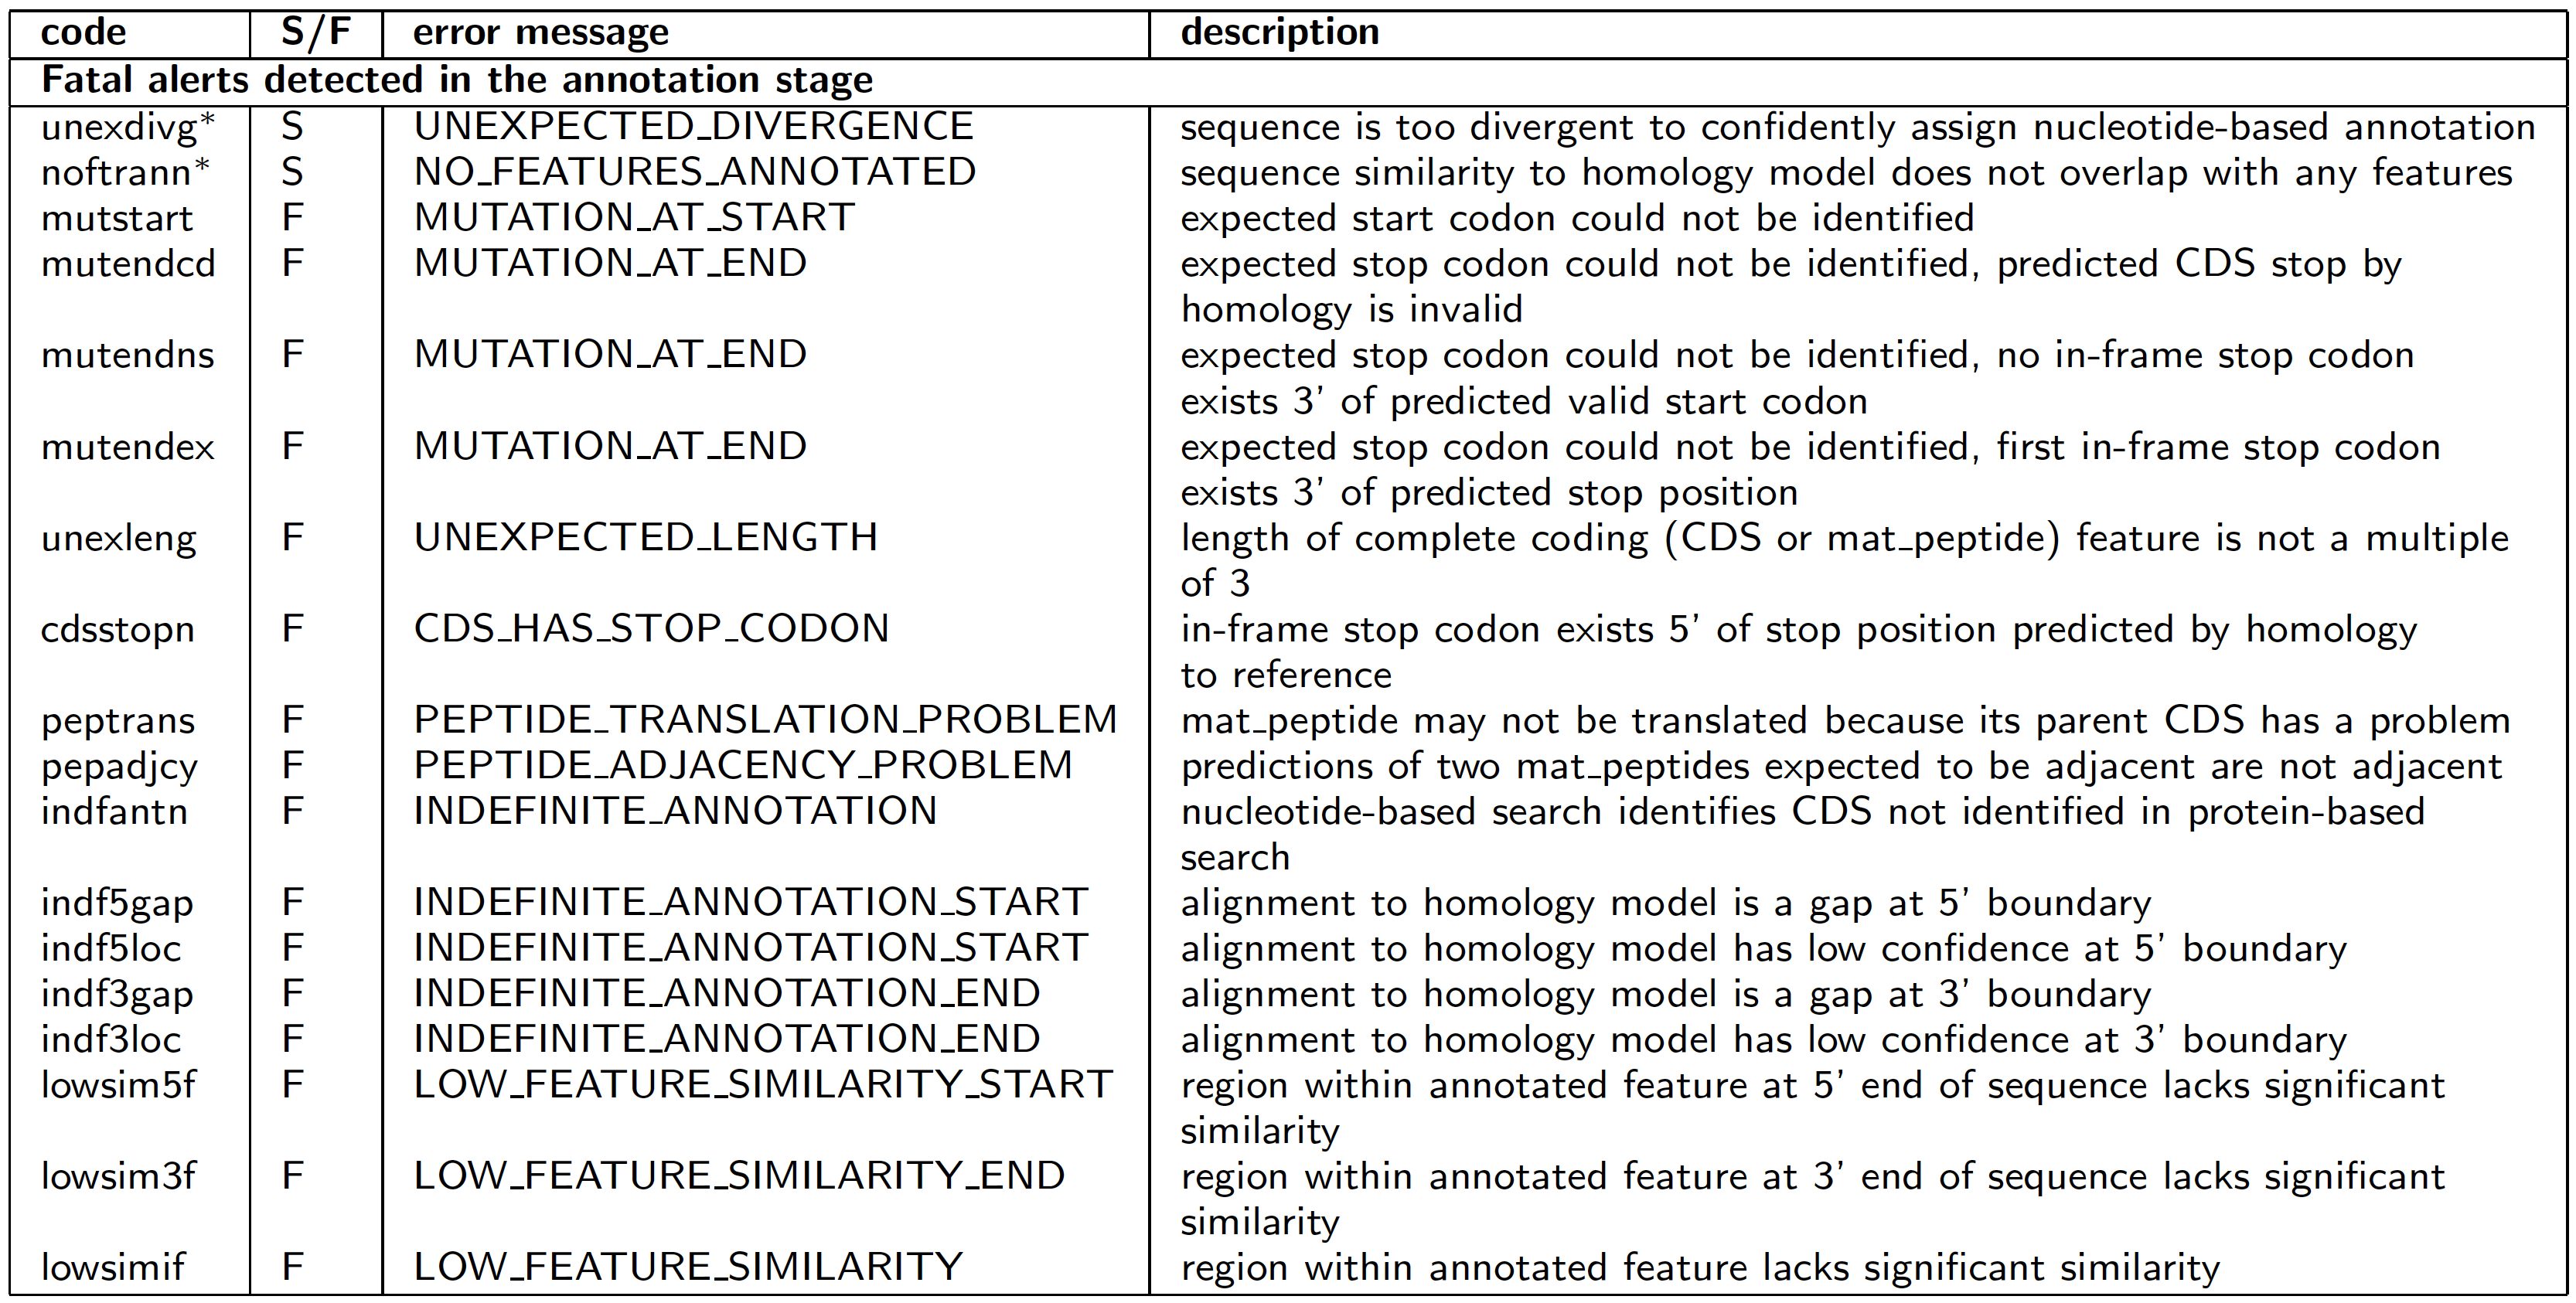
\includegraphics[width=10.5in]{figs/ss-alignment-alert-list}

\end{center}
\vfill
\end{slide}
%%%%%%%%%%%%%%%%%%%%%%%%%%%%%%%%%%%%%%%%%%%%%%%%%%%%%%%%%%%%%%%%%%%%%%
\begin{slide}
\begin{center}

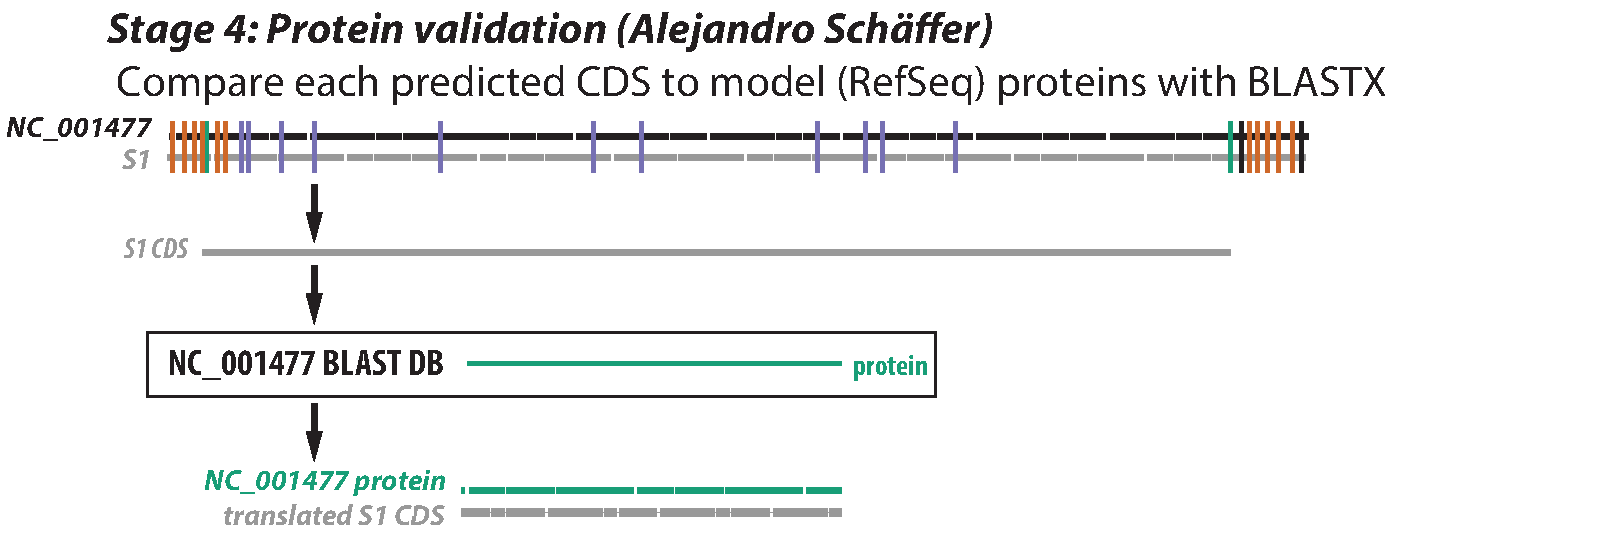
\includegraphics[width=10.5in]{figs/v-annotate-stage4-1}

\end{center}
\vfill
\end{slide}
%%%%%%%%%%%%%%%%%%%%%%%%%%%%%%%%%%%%%%%%%%%%%%%%%%%%%%%%%%%%%%%%%%%%%%
\begin{slide}
\begin{center}

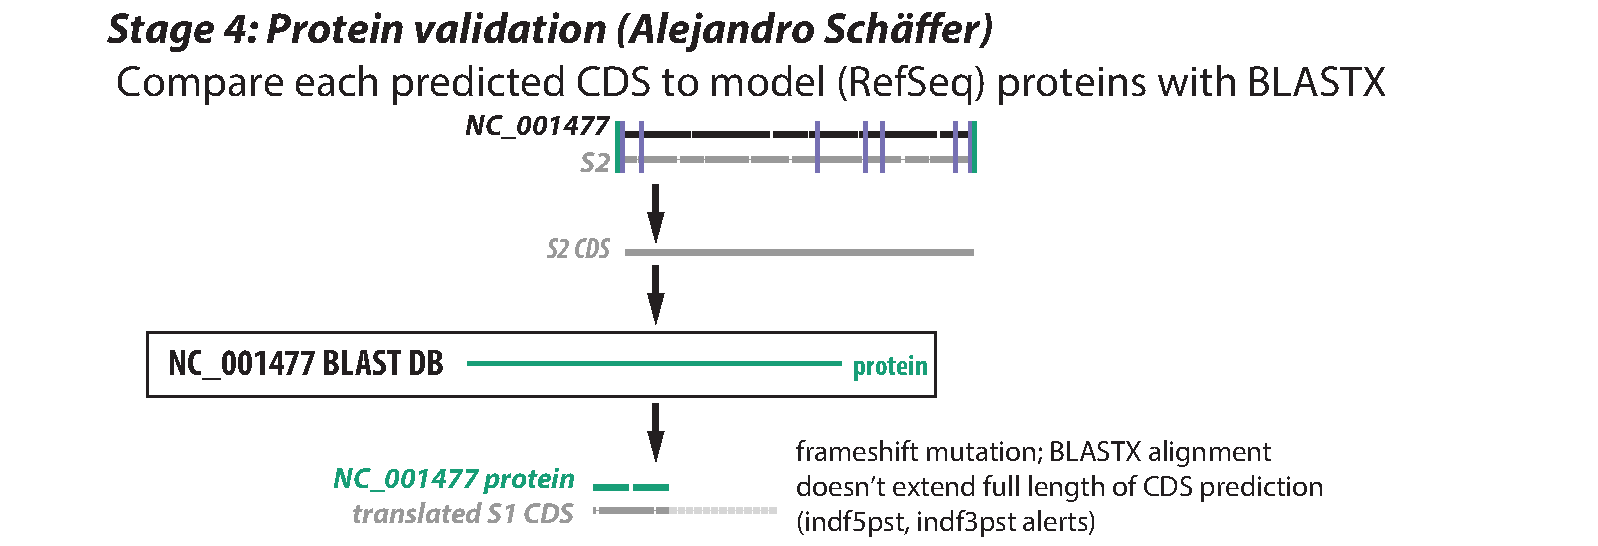
\includegraphics[width=10.5in]{figs/v-annotate-stage4-2}
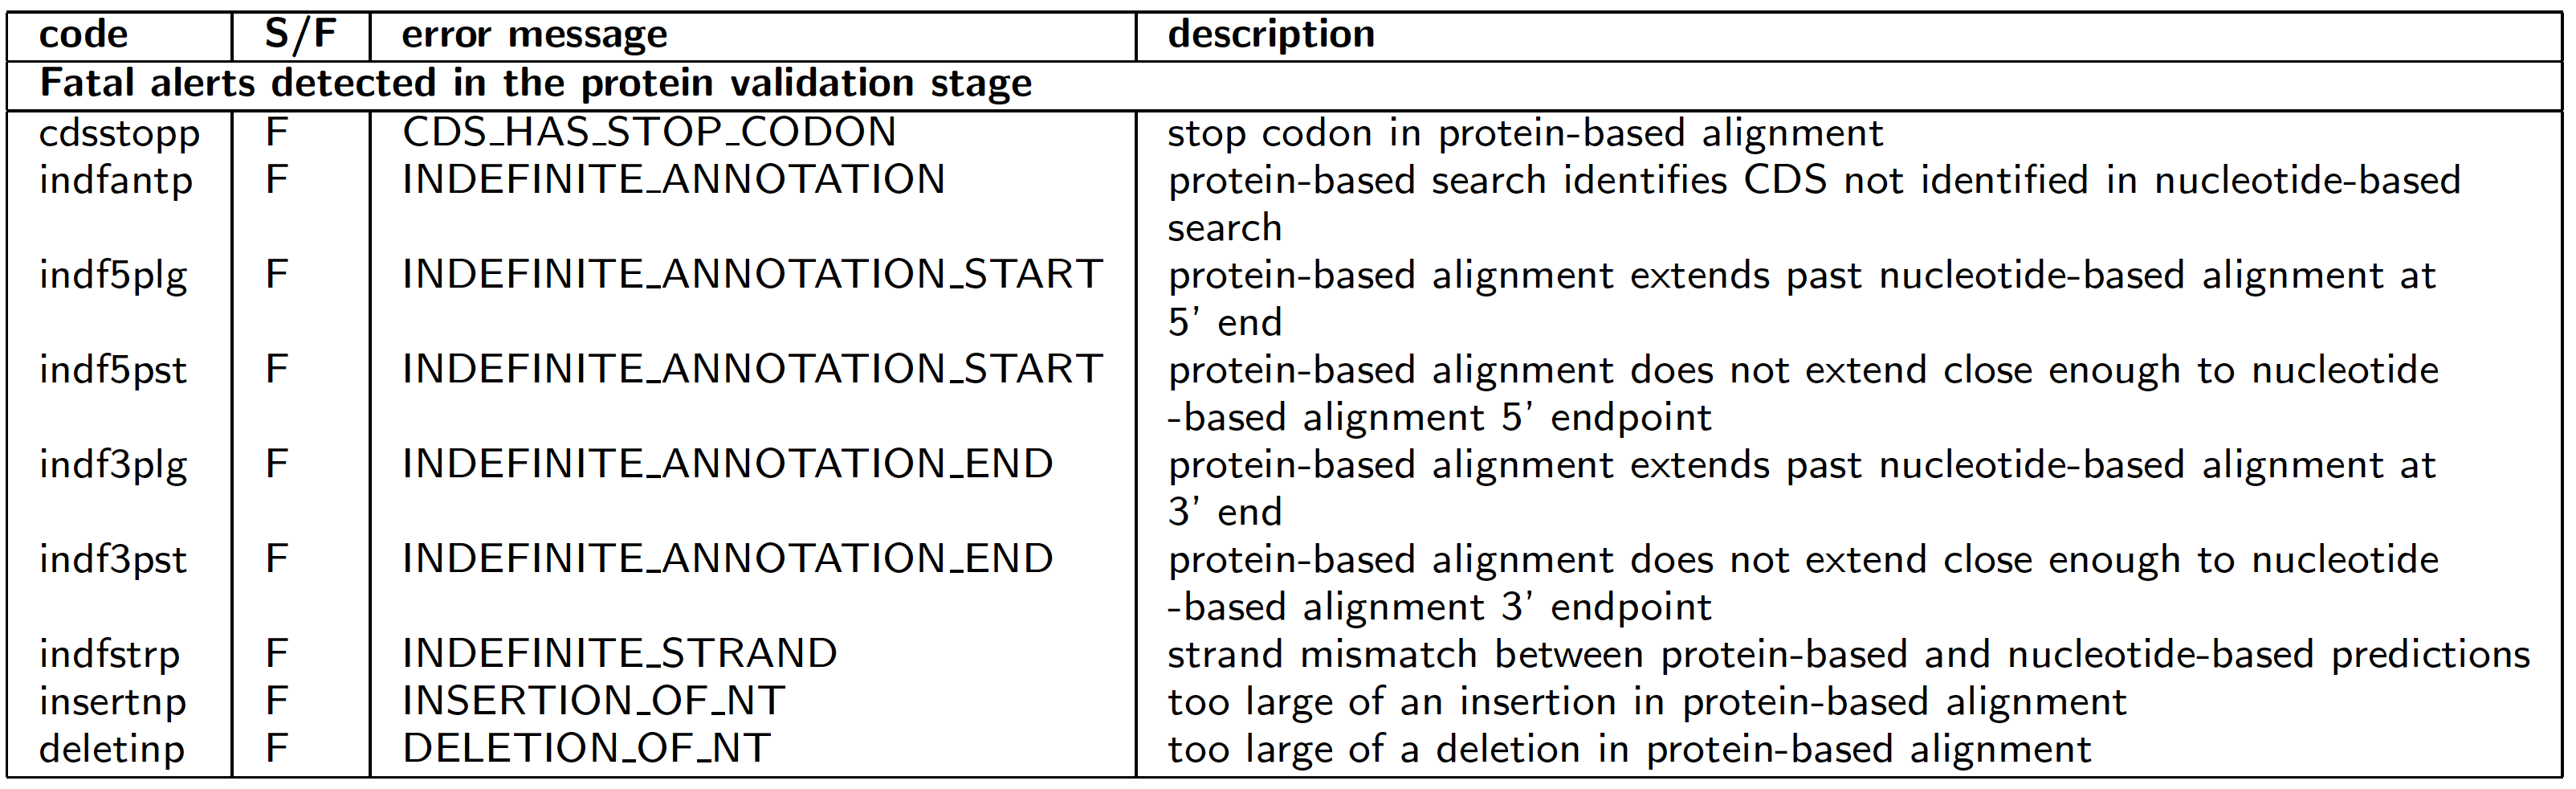
\includegraphics[width=10.5in]{figs/ss-protein-alert-list}

\end{center}
\vfill
\end{slide}
%%%%%%%%%%%%%%%%%%%%%%%%%%%%%%%%%%%%%%%%%%%%%%%%%%%%%%%%%%%%%%%%%%%%%%
%%%%%%%%%%%%%%%%%%%%%%%%%%%%%%%%%%%%%%%%%%%%%%%%%%%%%%%%%%%%%%%%%%%%%%
%%%%%%%%%%%%%%%%%%%%%%%%%%%%%%%%%%%%%%%%%%%%%%%%%%%%%%%%%%%%%%%%%%%%%%
\begin{comment}
\begin{slide}
\begin{center}
%\textbf{\texttt{v-annotate.pl} annotates each sequence using its
\textbf{VADR proceeds over four stages to validate and annotate sequences}

\begin{itemize}
\item For each sequence $S$:
\small
\begin{enumerate}
\item \textbf{Classification}: compare $S$ to all models to find best matching model $M$
\item \textbf{Coverage determination}: search $M$ against $S$ to find 'hits'
\item \textbf{Alignment}: align $S$ to $M$ and map features from $M$ to $S$
\item \textbf{Protein validation}: compare predicted CDS in $S$ to proteins
  from $M$ using BLASTX
\end{enumerate}
\end{itemize}

\emph{Different types of alerts are identified and reported at each stage}

\end{center}

\vfill
\end{slide}
%%%%%%%%%%%%%%%%%%%%%%%%%%%%%%%%%%%%%%%%%%%%%%%%%%%%%%%%%%%%%%%%%%%%%%
\begin{slide}
\begin{center}

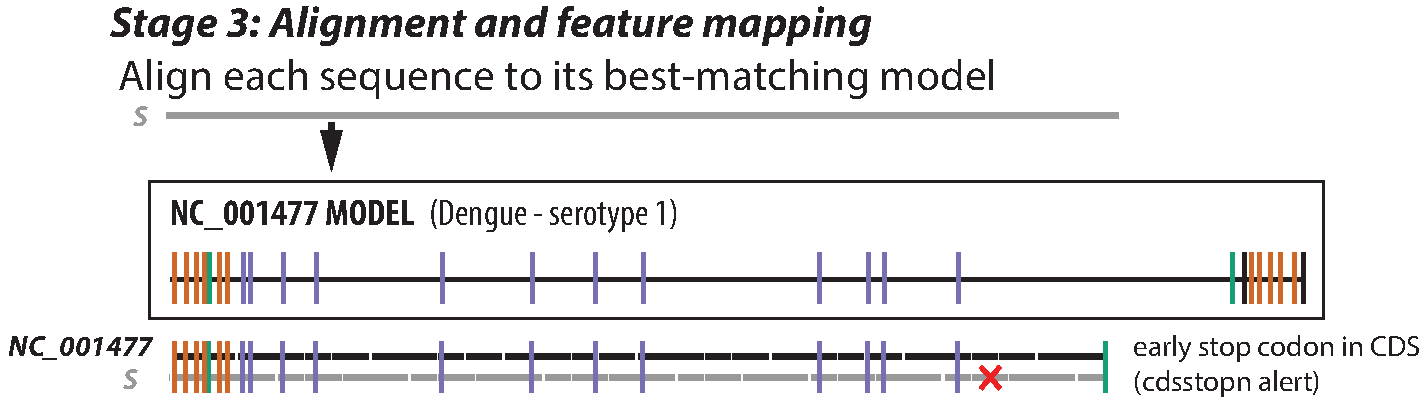
\includegraphics[width=10.5in]{figs/v-annotate-alignment-single-slide}

\end{center}
\vfill
\end{slide}
%%%%%%%%%%%%%%%%%%%%%%%%%%%%%%%%%%%%%%%%%%%%%%%%%%%%%%%%%%%%%%%%%%%%%%
\begin{slide}
\begin{center}

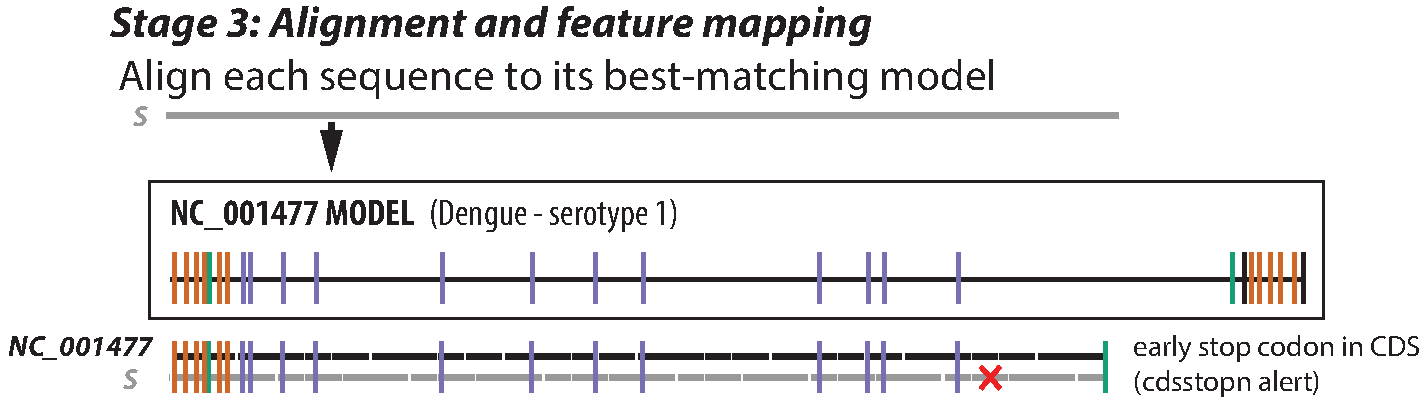
\includegraphics[width=10.5in]{figs/v-annotate-alignment-single-slide}
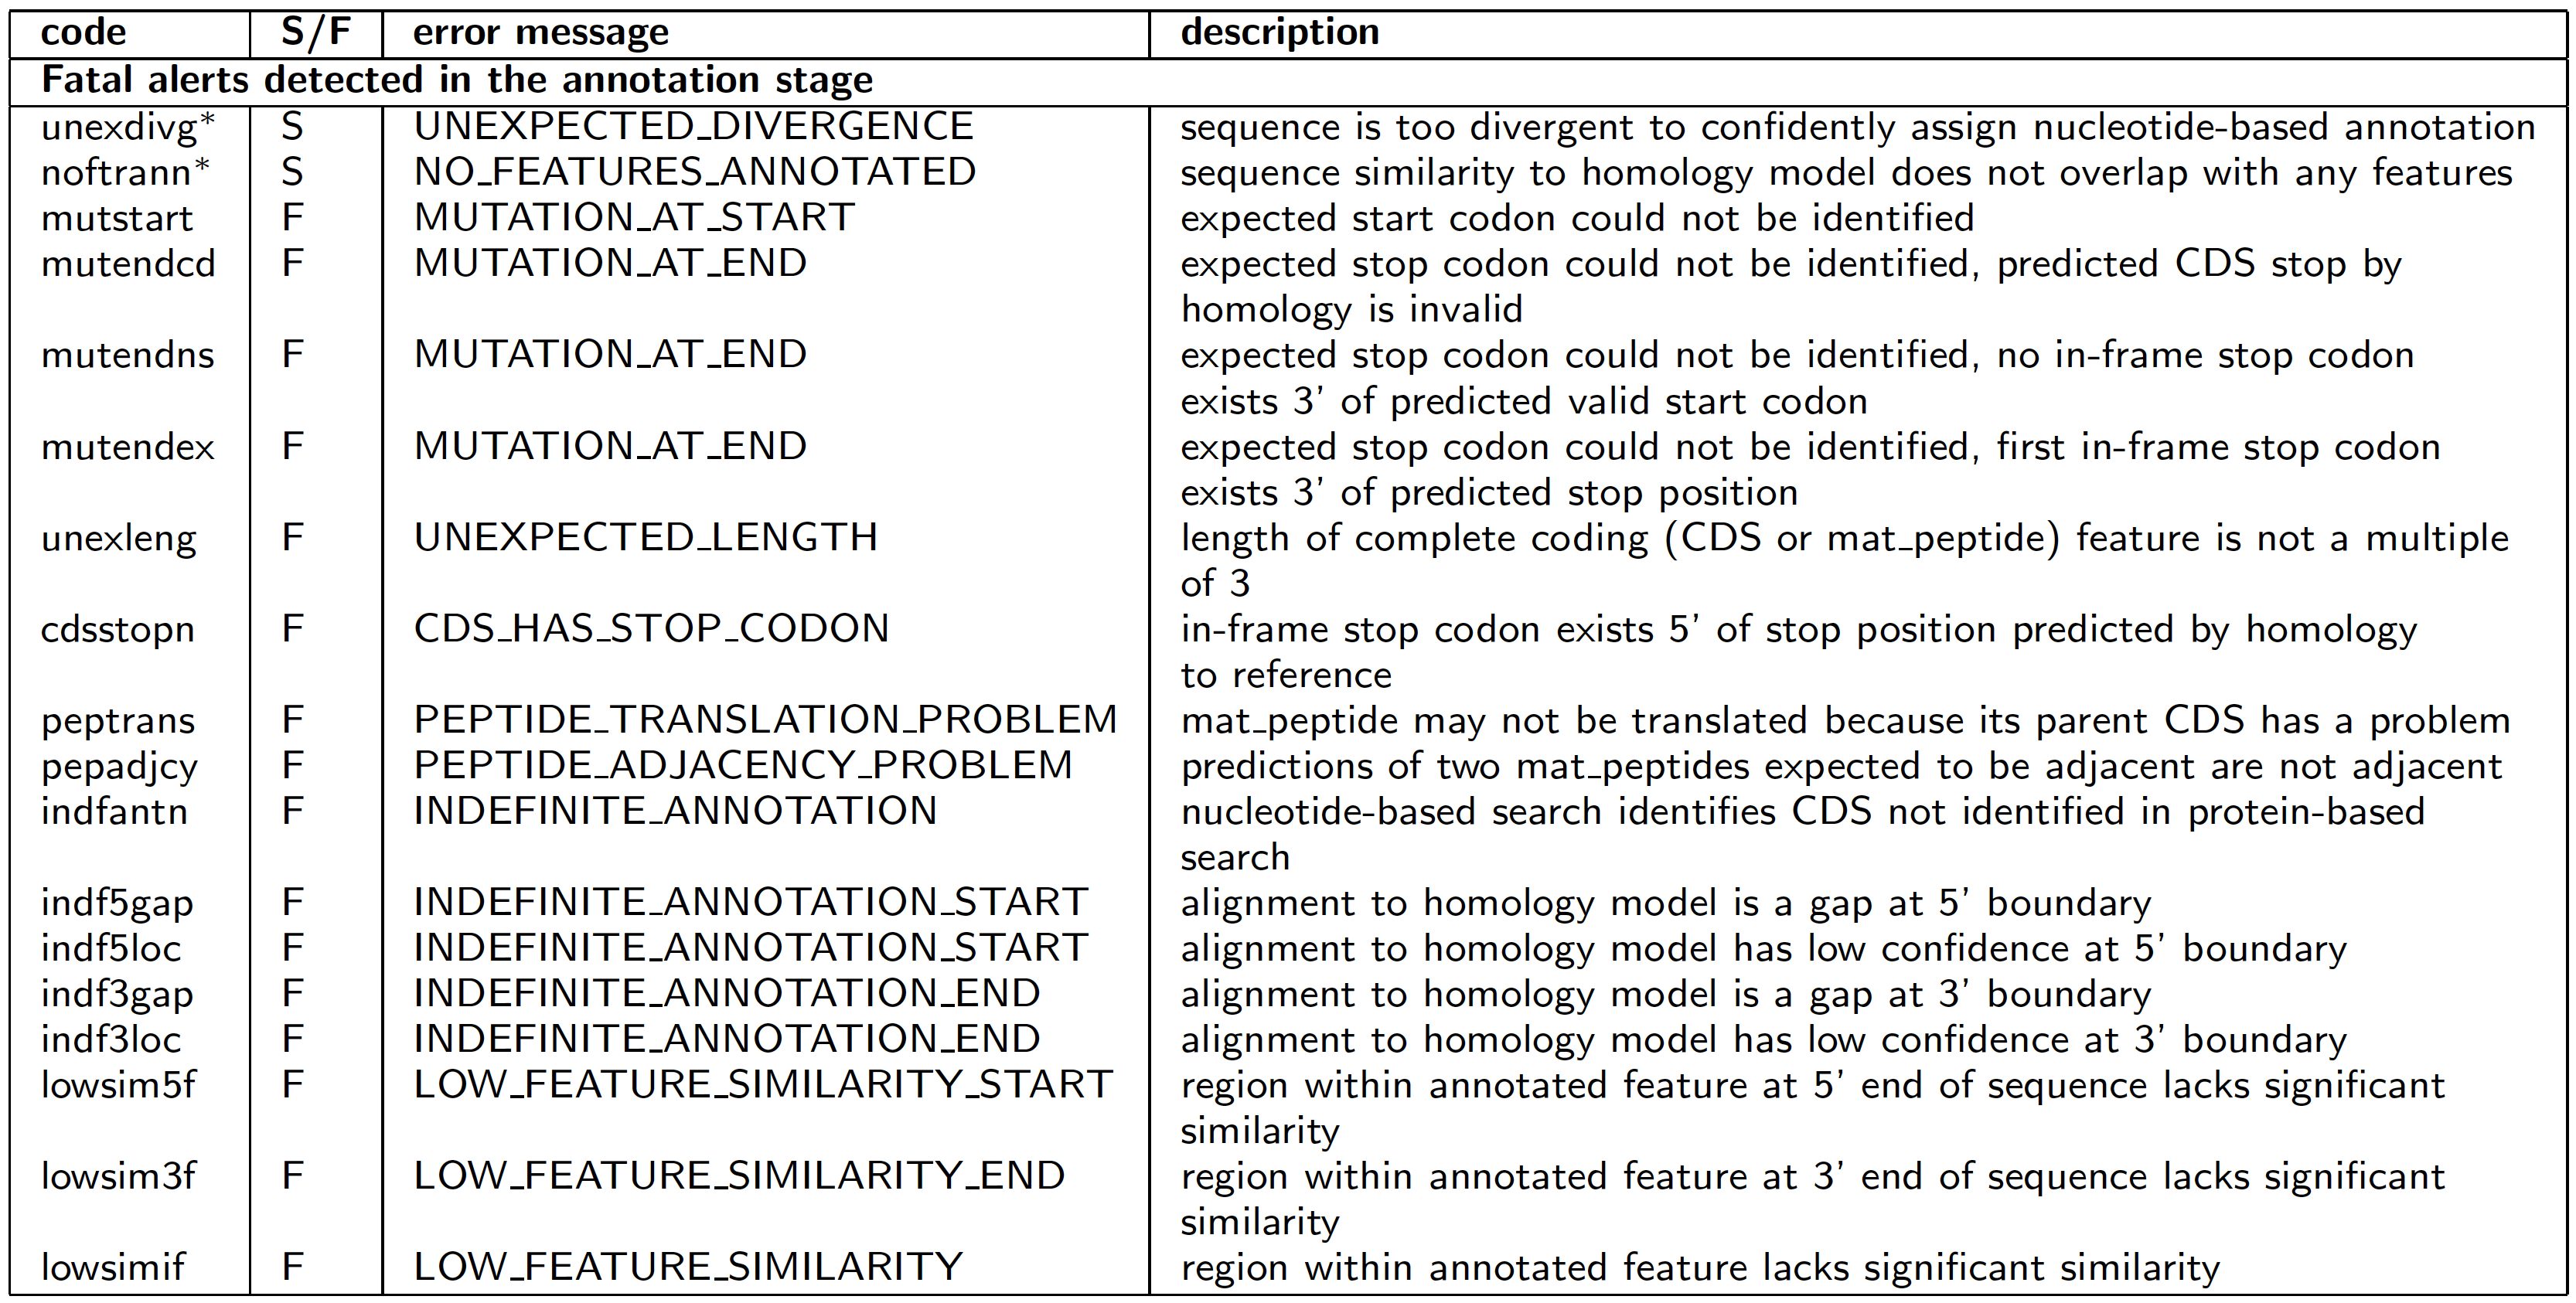
\includegraphics[width=10.5in]{figs/ss-alignment-alert-list}

\end{center}
\vfill
\end{slide}
%%%%%%%%%%%%%%%%%%%%%%%%%%%%%%%%%%%%%%%%%%%%%%%%%%%%%%%%%%%%%%%%%%%%%%
\end{comment}
%%%%%%%%%%%%%%%%%%%%%%%%%%%%%%%%%%%%%%%%%%%%%%%%%%%%%%%%%%%%%%%%%%%%%%
%%%%%%%%%%%%%%%%%%%%%%%%%%%%%%%%%%%%%%%%%%%%%%%%%%%%%%%%%%%%%%%%%%%%%%
%%%%%%%%%%%%%%%%%%%%%%%%%%%%%%%%%%%%%%%%%%%%%%%%%%%%%%%%%%%%%%%%%%%%%%
\begin{slide}
\begin{center}
\normalsize{\textbf{VADR used for Norovirus and Dengue virus sequences since 2018}}

\scriptsize
\begin{tabular}{r|r|r}
                                                  &Norovirus      &Dengue virus   \\ \hline
length                                            &7.6Kb         &10.7Kb        \\
\# seqs                                           &44,936          &113,211         \\
\% seqs full length                               &5.1\%          &8.4\%          \\
\% Ns                                             &0.5\%          &0.2\%          \\
\% seqs with stretch of $>=50$ Ns                 &1.0\%          &0.4\%          \\
average \% identity                               &81.6\%         &94.4\%         \\ \hline
\multicolumn{3}{l}{} \\ 
\multicolumn{3}{l}{\textbf{VADR v1.0 performance}} \\ \hline
seconds per sequence                   &42.4           &92.6           \\
required RAM                           &8Gb            &8Gb            \\
total running time, CPU days           &1.1            &10.2           \\
\end{tabular}
\end{center}

\vfill
\end{slide}
%%%%%%%%%%%%%%%%%%%%%%%%%%%%%%%%%%%%%%%%%%%%%%%%%%%%%%%%%%%%%%%%%%%%%%
\begin{slide}
\begin{center}
\normalsize{\textbf{SARS-CoV-2 sequence submissions have increased since early 2020}}
\end{center}

\tiny
\begin{center}
\begin{tabular}{llrr}
          &          &\#new     &\#cumulative\\
month     &year      &seqs      &seqs      \\ \hline
Jan       & 2020     &32        &32        \\ 
Feb       & 2020     &58        &90        \\ 
Mar       & 2020     &332       &422       \\ 
Apr       & 2020     &1541      &1963      \\ 
May       & 2020     &2974      &4937      \\ 
Jun       & 2020     &3394      &8331      \\ 
Jul       & 2020     &3604      &11,935    \\ 
Aug       & 2020     &3818      &15,753    \\ 
Sep       & 2020     &6731      &22,484    \\ 
Oct       & 2020     &11,939    &34,423    \\ 
Nov       & 2020     &4274      &38,697    \\ 
Dec       & 2020     &4530      &43,227    \\ 
& & & \\
Jan       & 2021     &8775      &52,002    \\ 
Feb       & 2021     &26,078    &78,080    \\ 
Mar       & 2021     &42,607    &120,687   \\ 
Apr       & 2021     &97,095    &217,782   \\ 
May       & 2021     &104,729   &322,511   \\ 
Jun       & 2021     &46,187    &368,698   \\ 
Jul       & 2021     &43,336    &412,034   \\ 
Aug       & 2021     &141,958   &553,992   \\ 
Sep       & 2021     &267,562   &821,554   \\ 
Oct       & 2021     &239,296   &1,060,850 \\ 
Nov       & 2021     &267,270   &1,328,120 \\ 
Dec       & 2021     &288,771   &1,616,891 \\ 
& & & \\
Jan       & 2022     &258,522   &1,875,413 \\ 
Feb       & 2022     &230,185   &2,105,598 \\ 
\end{tabular}
\end{center}

\vfill
\end{slide}
%%%%%%%%%%%%%%%%%%%%%%%%%%%%%%%%%%%%%%%%%%%%%%%%%%%%%%%%%%%%%%%%%%%%%%
\begin{slide}
\begin{center}
\normalsize{\textbf{SARS-CoV-2 sequences differ from Norovirus and Dengue virus \\ in several ways that impact VADR processing}}

\scriptsize
\begin{tabular}{r|r|r|r}
                                                  &Norovirus      &Dengue virus   &\textcolor{red}{SARS-CoV-2}      \\ \hline
length                                            &7.6Kb         &10.7Kb       &\textcolor{red}{29.9Kb}        \\
\# seqs                                           &44,936          &113,211         &\textcolor{red}{1,616,891}        \\
\% seqs full length                               &5.1\%          &8.4\%          &\textcolor{red}{99.7\%}         \\
\% Ns                                             &0.5\%          &0.2\%          &\textcolor{red}{1.4\%}          \\
\% seqs with stretch of $>=50$ Ns                 &1.0\%          &0.4\%          &\textcolor{red}{38.7\%}         \\
average \% identity                               &81.6\% &94.4\%         &\textcolor{red}{99.4\%}         \\ \hline
\multicolumn{4}{l}{} \\ 
\multicolumn{4}{l}{\textbf{VADR v1.0 performance}} \\ \hline
seconds per sequence                   &42.4           &92.6           &\textcolor{red}{331.8}          \\
required RAM                           &8Gb            &8Gb            &\textcolor{red}{64Gb}           \\
total running time, CPU days           &1.1            &10.2           &\textcolor{red}{6187.6}         \\
\end{tabular}
\end{center}

\vfill
\end{slide}
%%%%%%%%%%%%%%%%%%%%%%%%%%%%%%%%%%%%%%%%%%%%%%%%%%%%%%%%%%%%%%%%%%%%%%
\begin{slide}
\begin{center}
\normalsize{\textbf{Replacing Ns with expected nucleotides allows \\ many 'good' sequences to pass}}

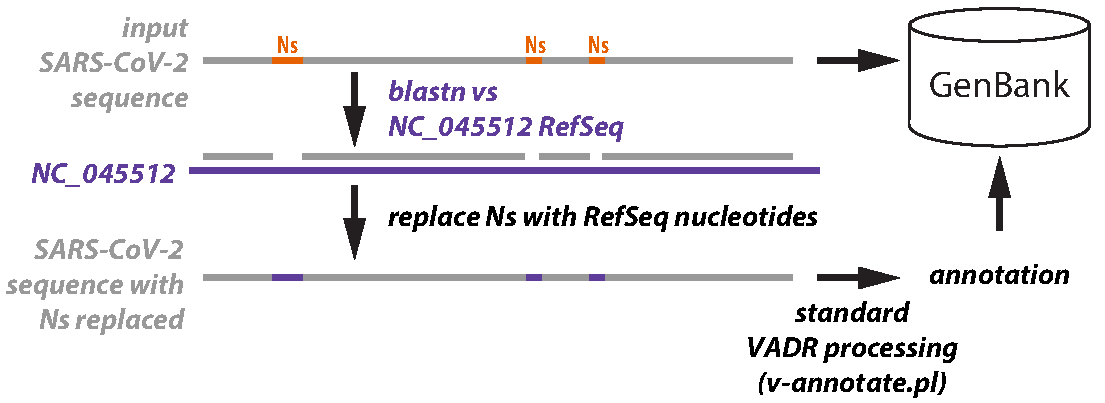
\includegraphics[width=10.25in]{figs/vadr-r-option}
\end{center}

\vfill
\end{slide}
%%%%%%%%%%%%%%%%%%%%%%%%%%%%%%%%%%%%%%%%%%%%%%%%%%%%%%%%%%%%%%%%%%%%%%
\begin{slide}
\begin{center}
\normalsize{\textbf{Seeded alignment using blastn makes alignment stage faster}}

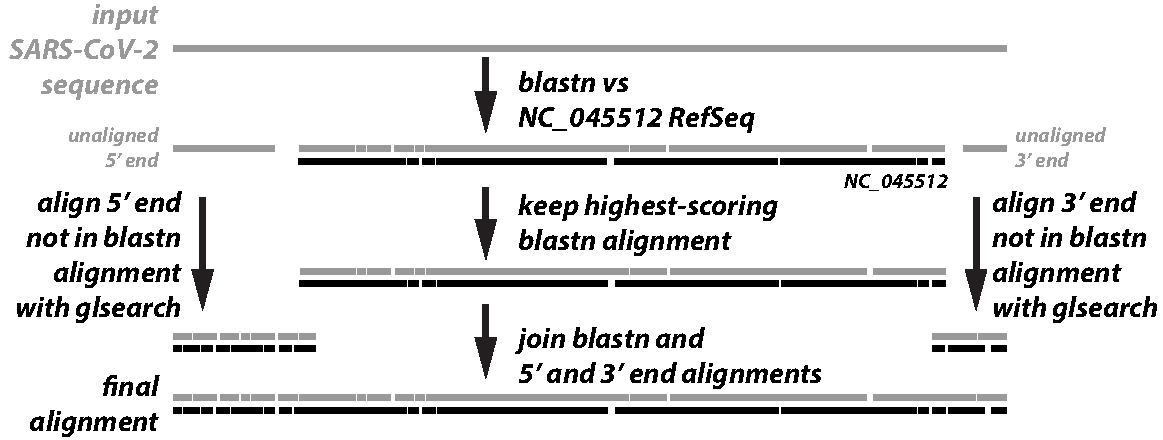
\includegraphics[width=10.25in]{figs/vadr-s-option}
\end{center}

\vfill
\end{slide}
%%%%%%%%%%%%%%%%%%%%%%%%%%%%%%%%%%%%%%%%%%%%%%%%%%%%%%%%%%%%%%%%%%%%%%
\begin{slide}
\begin{center}
\textbf{Using glsearch instead of cmalign reduces memory requirement}
\end{center}

\begin{itemize}
\item lower memory requirement (2Gb max) allows for multi-threading
%  \item input file is split into chunks
%    \begin{itemize}
%    \item each chunk processed independently in parallel on one of 8 CPUs
%    \item further reduces memory requirement for large input files \\ (dependent on chunk size
%      instead of input file size)
%    \end{itemize}
\end{itemize}

\begin{center}
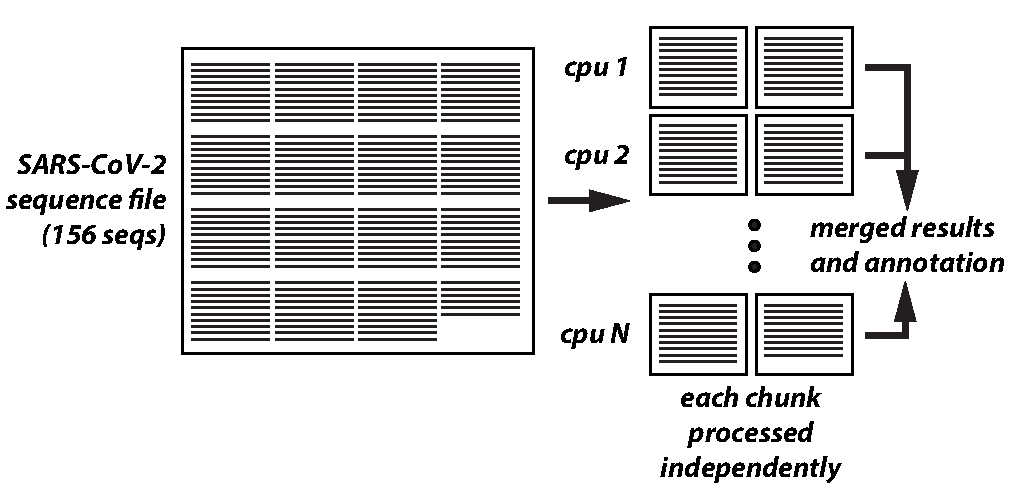
\includegraphics[width=10.5in]{figs/vadr-1p2-multithreading}
\end{center}
  
\vfill
\end{slide}
%%%%%%%%%%%%%%%%%%%%%%%%%%%%%%%%%%%%%%%%%%%%%%%%%%%%%%%%%%%%%%%%%%%%%%
\begin{comment}
\begin{slide}
\begin{center}
\normalsize{\textbf{VADR is now 1000-fold faster in practice for SARS-CoV-2 processing}}

\scriptsize
\begin{tabular}{lrrrrrrrr}
            &seeded      &N           &            &            &            &secs        &hours       &speedup     \\ 
VADR        &align-      &replace-    &            &\#          &required    &per         &per 100K    &vs          \\ 
version     &ment?       &ment?       &glsearch?   &cpus        &RAM         &seq         &seqs        &v1.0        \\ 
\hline
& & & & & & & & \\
v1.0        &$-$         &$-$         &$-$         &1           &64 Gb       &329.91      &9164.3      &-           \\
\end{tabular}
\end{center}

\vfill
\end{slide}
%%%%%%%%%%%%%%%%%%%%%%%%%%%%%%%%%%%%%%%%%%%%%%%%%%%%%%%%%%%%%%%%%%%%%%
\begin{slide}
\begin{center}
\normalsize{\textbf{VADR is now 1000-fold faster in practice for SARS-CoV-2 processing}}

\scriptsize
\begin{tabular}{lrrrrrrrr}
            &seeded      &N           &            &            &            &secs        &hours       &speedup     \\ 
VADR        &align-      &replace-    &            &\#          &required    &per         &per 100K    &vs          \\ 
version     &ment?       &ment?       &glsearch?   &cpus        &RAM         &seq         &seqs        &v1.0        \\ 
\hline
& & & & & & & & \\
v1.0         &$-$         &$-$         &$-$         &1           &64 Gb       &329.91      &9164.3      &-           \\
%1.1         &$+$         &$+$         &$-$         &1           &64 Gb       &49.35       &1370.7      &6.7         \\
& & & & & & & & \\
v1.4.1       &$+$         &$+$         &$+$         &1           &2 Gb        &2.51        &69.8        &131.4       \\
\end{tabular}
\end{center}

\vfill
\end{slide}
\end{comment}
%%%%%%%%%%%%%%%%%%%%%%%%%%%%%%%%%%%%%%%%%%%%%%%%%%%%%%%%%%%%%%%%%%%%%%
\begin{slide}
\begin{center}
\normalsize{\textbf{VADR is now 1000-fold faster in practice for SARS-CoV-2 processing}}

\scriptsize
\begin{tabular}{lrrrrrrrr}
            &seeded      &N           &            &            &            &secs        &hours       &speedup     \\ 
VADR        &align-      &replace-    &            &\#          &required    &per         &per 100K    &vs          \\ 
version     &ment?       &ment?       &glsearch?   &cpus        &RAM         &seq         &seqs        &v1.0        \\ 
\hline
& & & & & & & & \\
v1.0         &$-$         &$-$         &$-$         &1           &64 Gb       &329.91      &9164.3      &-           \\
%v1.1         &$+$         &$+$         &$-$         &1           &64 Gb       &49.35       &1370.7      &6.7         \\
%& & & & & & & & \\
%v1.4.1       &$+$         &$+$         &$+$         &1           &2 Gb        &2.51        &69.8        &131.4       \\
%& & & & & & & & \\
%v1.4.1       &$+$         &$+$         &$+$         &2           &4 Gb        &1.49        &41.5        &220.8       \\
%& & & & & & & & \\
%v1.4.1       &$+$         &$+$         &$+$         &4           &8 Gb        &0.65        &18.0        &509.9       \\
& & & & & & & & \\
\textbf{v1.4.1}&\textbf{$+$}&\textbf{$+$}&\textbf{$+$}&\textbf{8}  &\textbf{16 Gb}&\textbf{0.33}&\textbf{9.3}&\textbf{986.8}\\
%& & & & & & & & \\
%v1.4.1       &$+$         &$+$         &$+$         &16          &32 Gb       &0.23        &6.5         &1417.9      \\
%& & & & & & & & \\
%v1.4.1       &$+$         &$+$         &$+$         &32          &64 Gb       &0.13        &3.7         &2462.2      \\
\end{tabular}
\end{center}

\vfill
\end{slide}
%%%%%%%%%%%%%%%%%%%%%%%%%%%%%%%%%%%%%%%%%%%%%%%%%%%%%%%%%%%%%%%%%%%%%%
\begin{slide}
\begin{center}
\normalsize{\textbf{VADR is now fast enough to handle \\ hundreds of thousands of sequences per month}}
\end{center}

\tiny
\begin{center}
\begin{tabular}{llrr}
          &          &\#new     &\#cumulative\\
month     &year      &seqs      &seqs      \\ \hline
Jan       & 2020     &32        &32        \\ 
Feb       & 2020     &58        &90        \\ 
Mar       & 2020     &332       &422       \\ 
Apr       & 2020     &1541      &1963      \\ 
May       & 2020     &2974      &4937      \\ 
Jun       & 2020     &3394      &8331      \\ 
Jul       & 2020     &3604      &11,935    \\ 
Aug       & 2020     &3818      &15,753    \\ 
Sep       & 2020     &6731      &22,484    \\ 
Oct       & 2020     &11,939    &34,423    \\ 
Nov       & 2020     &4274      &38,697    \\ 
Dec       & 2020     &4530      &43,227    \\ 
& & & \\
Jan       & 2021     &8775      &52,002    \\ 
Feb       & 2021     &26,078    &78,080    \\ 
Mar       & 2021     &42,607    &120,687   \\ 
Apr       & 2021     &97,095    &217,782   \\ 
May       & 2021     &104,729   &322,511   \\ 
Jun       & 2021     &46,187    &368,698   \\ 
Jul       & 2021     &43,336    &412,034   \\ 
Aug       & 2021     &141,958   &553,992   \\ 
Sep       & 2021     &267,562   &821,554   \\ 
Oct       & 2021     &239,296   &1,060,850 \\ 
Nov       & 2021     &267,270   &1,328,120 \\ 
Dec       & 2021     &288,771   &1,616,891 \\ 
& & & \\
Jan       & 2022     &258,522   &1,875,413 \\ 
Feb       & 2022     &230,185   &2,105,598 \\ 
\end{tabular}
\end{center}

\vfill
\end{slide}
%%%%%%%%%%%%%%%%%%%%%%%%%%%%%%%%%%%%%%%%%%%%%%%%%%%%%%%%%%%%%%%%%%%%%%
\begin{slide}
\begin{center}
\textbf{Besides getting faster, VADR has changed in other ways \\ (work with Linda Yankie and Vince Calhoun and GenBank team)}

\begin{itemize}
\item 13 releases between March 2020 and January 2022
\item 3 additional models (all eventually dropped):
  \begin{itemize}
  \item B.1.1.7 (alpha)
  \item B.1.525
  \item 28254-deletion
  \end{itemize}
\item allow some alerts for non-essential ORFs without failing sequence \\ (they become a \texttt{misc\_feature} instead)
\end{itemize}

\end{center}

\vfill
\end{slide}
%%%%%%%%%%%%%%%%%%%%%%%%%%%%%%%%%%%%%%%%%%%%%%%%%%%%%%%%%%%%%%%%%%%%%%
\begin{slide}
  \begin{center}
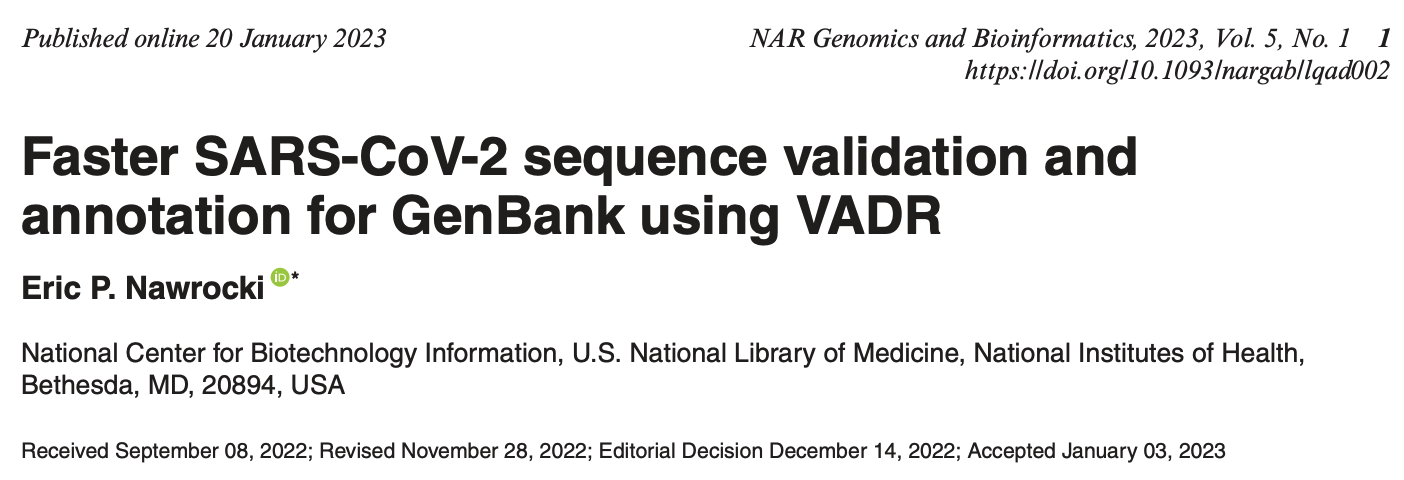
\includegraphics[width=10.5in]{figs/vadr-sarscov2-paper}
\end{center}

\vfill
\end{slide}
%%%%%%%%%%%%%%%%%%%%%%%%%%%%%%%%%%%%%%%%%%%%%%%%%%%%%%%%%%%%%%%%%%%%%%
\begin{slide}
  \begin{center}
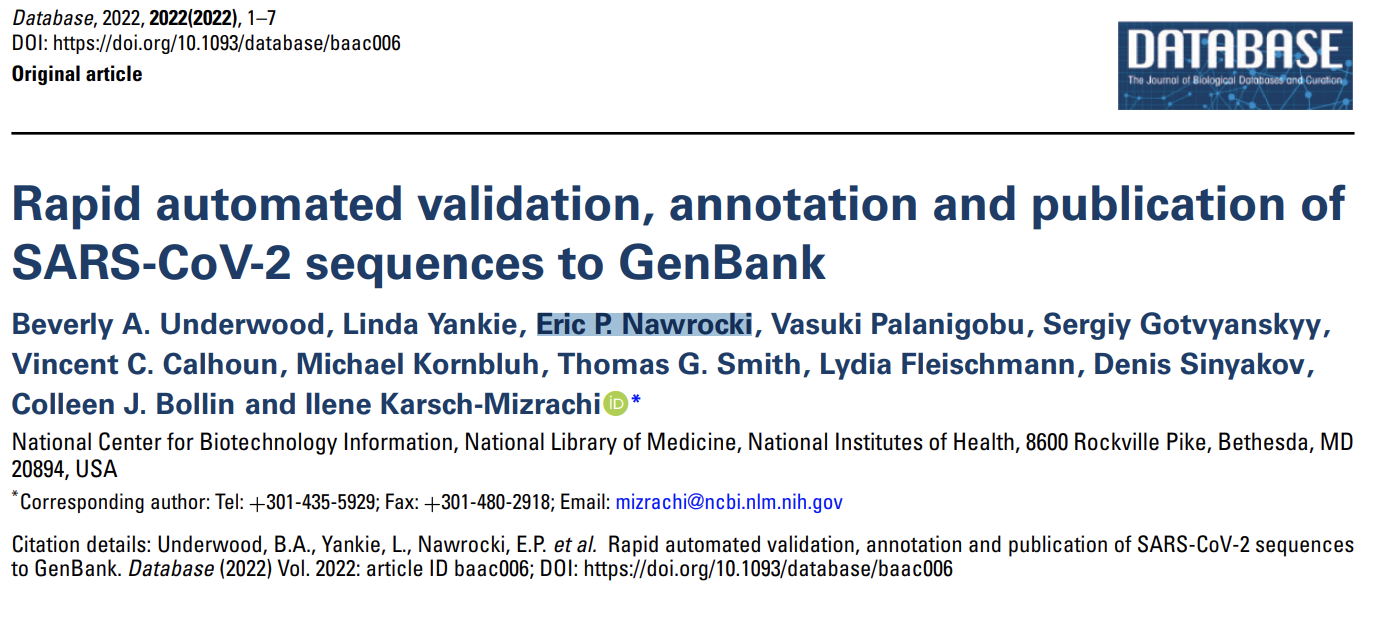
\includegraphics[width=10.5in]{figs/paper-genbank-covid}
\end{center}

\vfill
\end{slide}
%%%%%%%%%%%%%%%%%%%%%%%%%%%%%%%%%%%%%%%%%%%%%%%%%%%%%%%%%%%%%%%%%%%%%%
\begin{slide}
  \begin{center}

\includegraphics[height=7.5in]{figs/paper-covid}
\end{center}

\vfill
\end{slide}
%%%%%%%%%%%%%%%%%%%%%%%%%%%%%%%%%%%%%%%%%%%%%%%%%%%%%%%%%%%%%%%%%%%%%%
\begin{slide}
\begin{center}
  \textbf{Additional VADR models and development}

\small
\begin{tabular}{l|r|r|l|l|l}
 & length & num models & new feature(s) & author\\ \hline
 & & & & & \\ 
RSV & 15Kb & 2 & alignment-based models & Eric Nawrocki \\
 & & & & & \\ 
COX-1 & 1.5Kb & 86 & protein-coding gene & Eric Nawrocki \\
 & & & & & \\ 
Mpox & 197Kb & 1 & minimap alignment & Eric Nawrocki \\
 & & & & & \\ 
Influenza & 1-2Kb & 70 & segmented virus & Eric Nawrocki \\
 & & & & & \\ 
Zika      & 11Kb & ? & ? & EB Dickinson \\
\end{tabular}

% 
\includegraphics[width=10.5in]{figs/vadr-flu-paper}

\end{center}
  \vfill
\end{slide}
%%%%%%%%%%%%%%%%%%%%%%%%%%%%%%%%%%%%%%%%%%%%%%%%%%%%%%%%%%%%%%%%%%%%%%
\begin{slide}
\begin{center}
  \textbf{Additional VADR models and development}

\small
\begin{tabular}{l|r|r|l|l|l}
 & length & num models & new feature(s) & author\\ \hline
 & & & & & \\ 
RSV & 15Kb & 2 & alignment-based models & Eric Nawrocki \\
 & & & & & \\ 
COX-1 & 1.5Kb & 86 & protein-coding gene & Eric Nawrocki \\
 & & & & & \\ 
Mpox & 197Kb & 1 & minimap alignment & Eric Nawrocki \\
 & & & & & \\ 
Influenza & 1-2Kb & 70 & segmented virus & Eric Nawrocki \\
 & & & & & \\ 
Zika      & 11Kb & ? & ? & EB Dickinson \\
\end{tabular}


\includegraphics[width=10.5in]{figs/vadr-flu-paper}

\end{center}
  \vfill
\end{slide}
%%%%%%%%%%%%%%%%%%%%%%%%%%%%%%%%%%%%%%%%%%%%%%%%%%%%%%%%%%%%%%%%%%%%%%
\begin{slide}
\begin{center}
  \textbf{Additional VADR models and development}
\end{center}

%  \begin{itemize}
%  \item VADR is general, standalone and includes a module for users to
%    build new models 
\begin{itemize}
  \item Alex Greninger's lab at Univ of Washington:
    \begin {itemize}
    \item sequences a wide variety of human pathogenic viruses
    \item previously developed the VAPiD software tool for validating
      and annotating viral sequences
    \item now a collaborator that builds VADR models
  \end{itemize}
\end{itemize}

  \vfill
\end{slide}
%%%%%%%%%%%%%%%%%%%%%%%%%%%%%%%%%%%%%%%%%%%%%%%%%%%%%%%%%%%%%%%%%%%%%%
\begin{slide}
\begin{center}
  \textbf{Additional VADR models and development}

\small
\begin{tabular}{l|r|r|l|l|l}
 & length & num models & new feature(s) & author\\ \hline
 & & & & & \\ 
RSV & 15Kb & 2 & alignment-based models & Eric Nawrocki \\
 & & & & & \\ 
COX-1 & 1.5Kb & 86 & protein-coding gene & Eric Nawrocki \\
 & & & & & \\ 
Mpox & 197Kb & 1 & minimap alignment & Eric Nawrocki \\
 & & & & & \\ 
Influenza & 1-2Kb & 70 & segmented virus & Eric Nawrocki \\
 & & & & & \\ 
Zika      & 11Kb & ? & ? & EB Dickinson \\
 & & & & & \\ 
\textcolor{red}{Herpes Simplex} & \textcolor{red}{150Kb} & \textcolor{red}{2} & \textcolor{red}{-} & \textcolor{red}{Jaydee Sereewit} \\
\textcolor{red}{Virus (HSV)} &  &  & & \textcolor{red}{(Greninger Lab)} \\
 & & & & & \\ 
\textcolor{red}{Human meta-} & \textcolor{red}{13Kb} & \textcolor{red}{6} & \textcolor{red}{-} & \textcolor{red}{Jeffrey Furlong} \\
\textcolor{red}{pneumovirus (HMPV)} &  &  & & \textcolor{red}{(Greninger Lab)} \\
 & & & & & \\ 
\textcolor{red}{Human para-} & \textcolor{red}{15Kb} & \textcolor{red}{5} & \textcolor{red}{-} & \textcolor{red}{Jeffrey Furlong} \\
\textcolor{red}{influenza virus (HPIV)} &  &  &  & \textcolor{red}{(Greninger Lab)} \\
\end{tabular}

\end{center}
  \vfill
\end{slide}
%%%%%%%%%%%%%%%%%%%%%%%%%%%%%%%%%%%%%%%%%%%%%%%%%%%%%%%%%%%%%%%%%%%%%%
\begin{slide}
\begin{center}
  \textbf{Future directions for VADR}
\end{center}

  \begin{itemize}
  \item NCBI Virus FY2025 goals: 
    \begin{itemize}
    \item VADR web server
    \item Replacement of FLAN with VADR
    \end{itemize}

  \item Models for more viruses (our group and Greninger lab)
%  \item Alignment-based models 
%  \item RNA structure annotation in Flaviviruses (already exists for Dengue)
  \end{itemize}
  \vfill

\end{slide}
%%%%%%%%%%%%%%%%%%%%%%%%%%%%%%%%%%%%%%%%%%%%%%%%%%%%%%%%%%%%%%%%%%%%%%
%%%%%%%%%%%%%%%%%%%%%%%%%%%%%%%%%%%%%%%%%%%%%%%%%%%%%%%%%%%%%%%%%%%%
\begin{slide}
\center{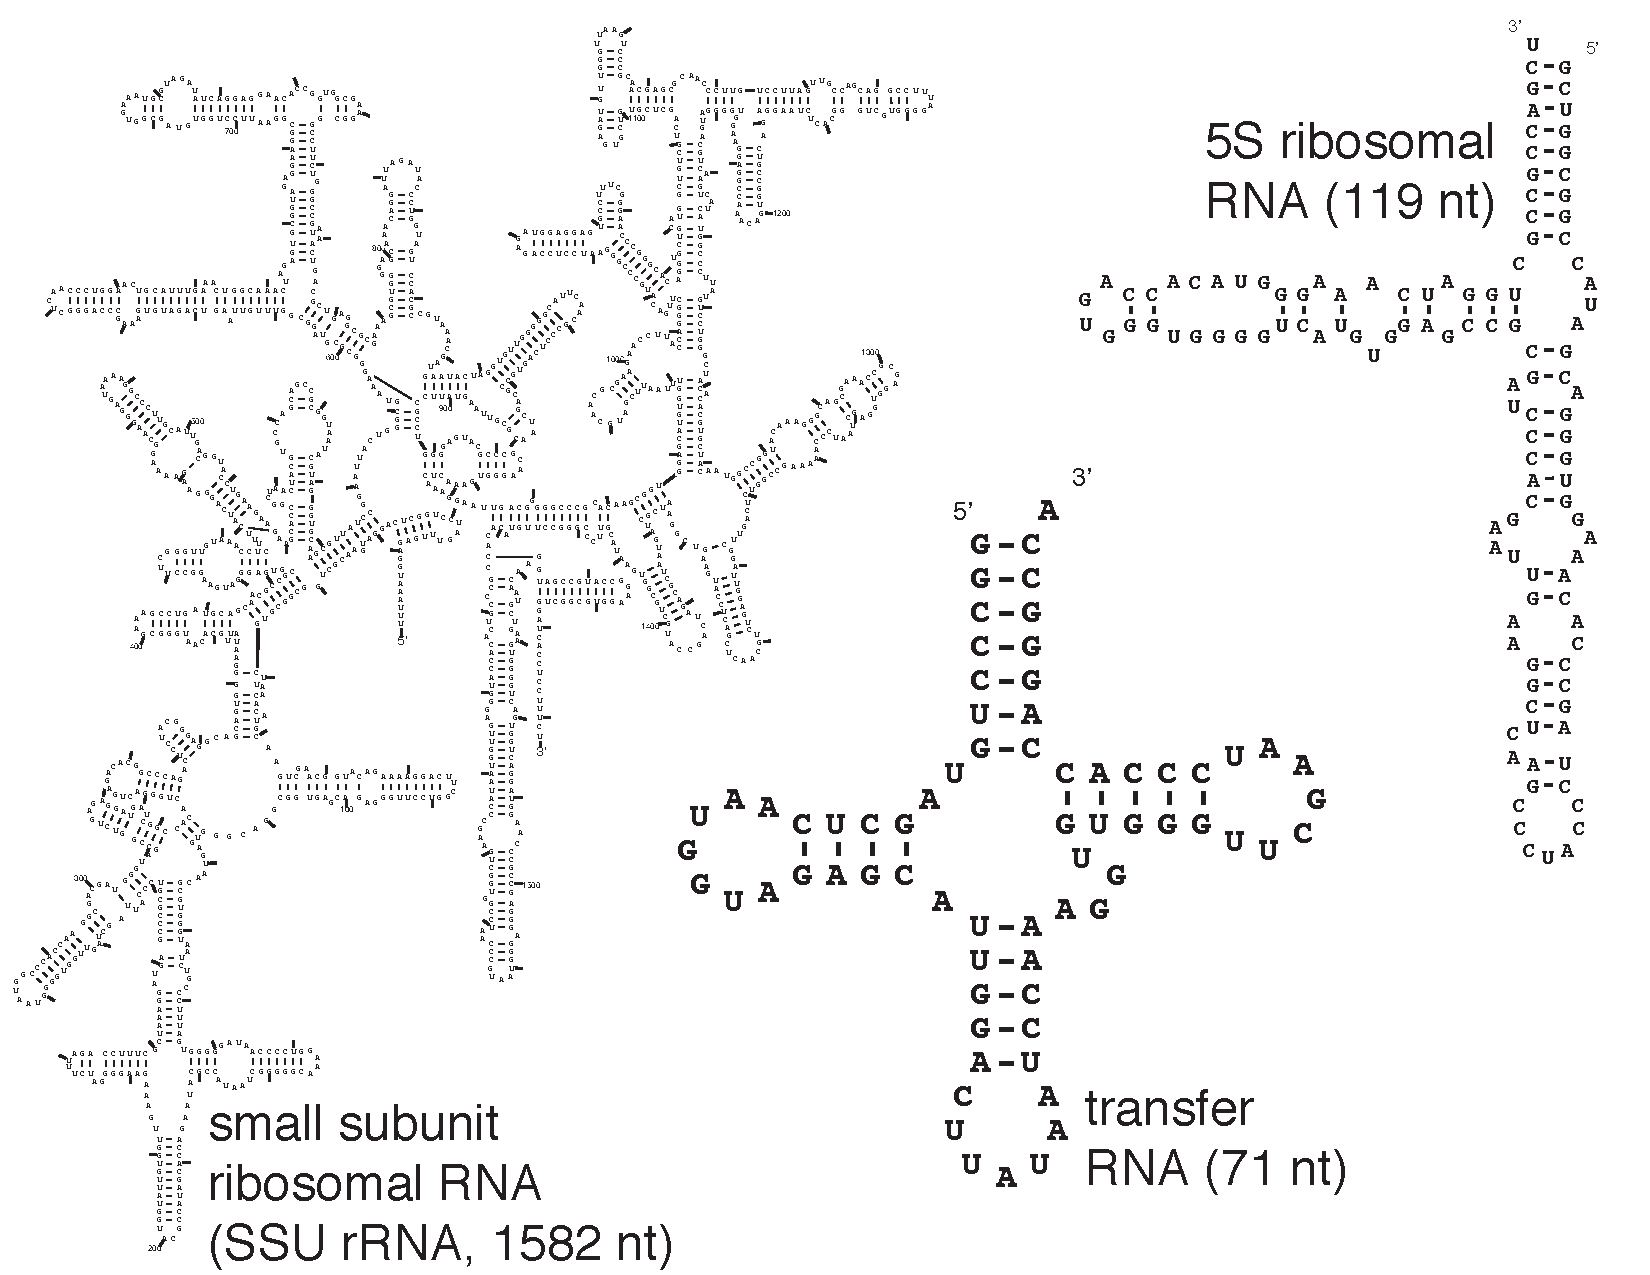
\includegraphics[width=10.5in]{figs/16s-5s-trna-allblack}}
\end{slide}
%%%%%%%%%%%%%%%%%%%%%%%%%%%%%%%%%%%%%%%%%%%%%%%%%%%%%%%%%%%%%%%%%%%%
%\begin{slide}
%\center{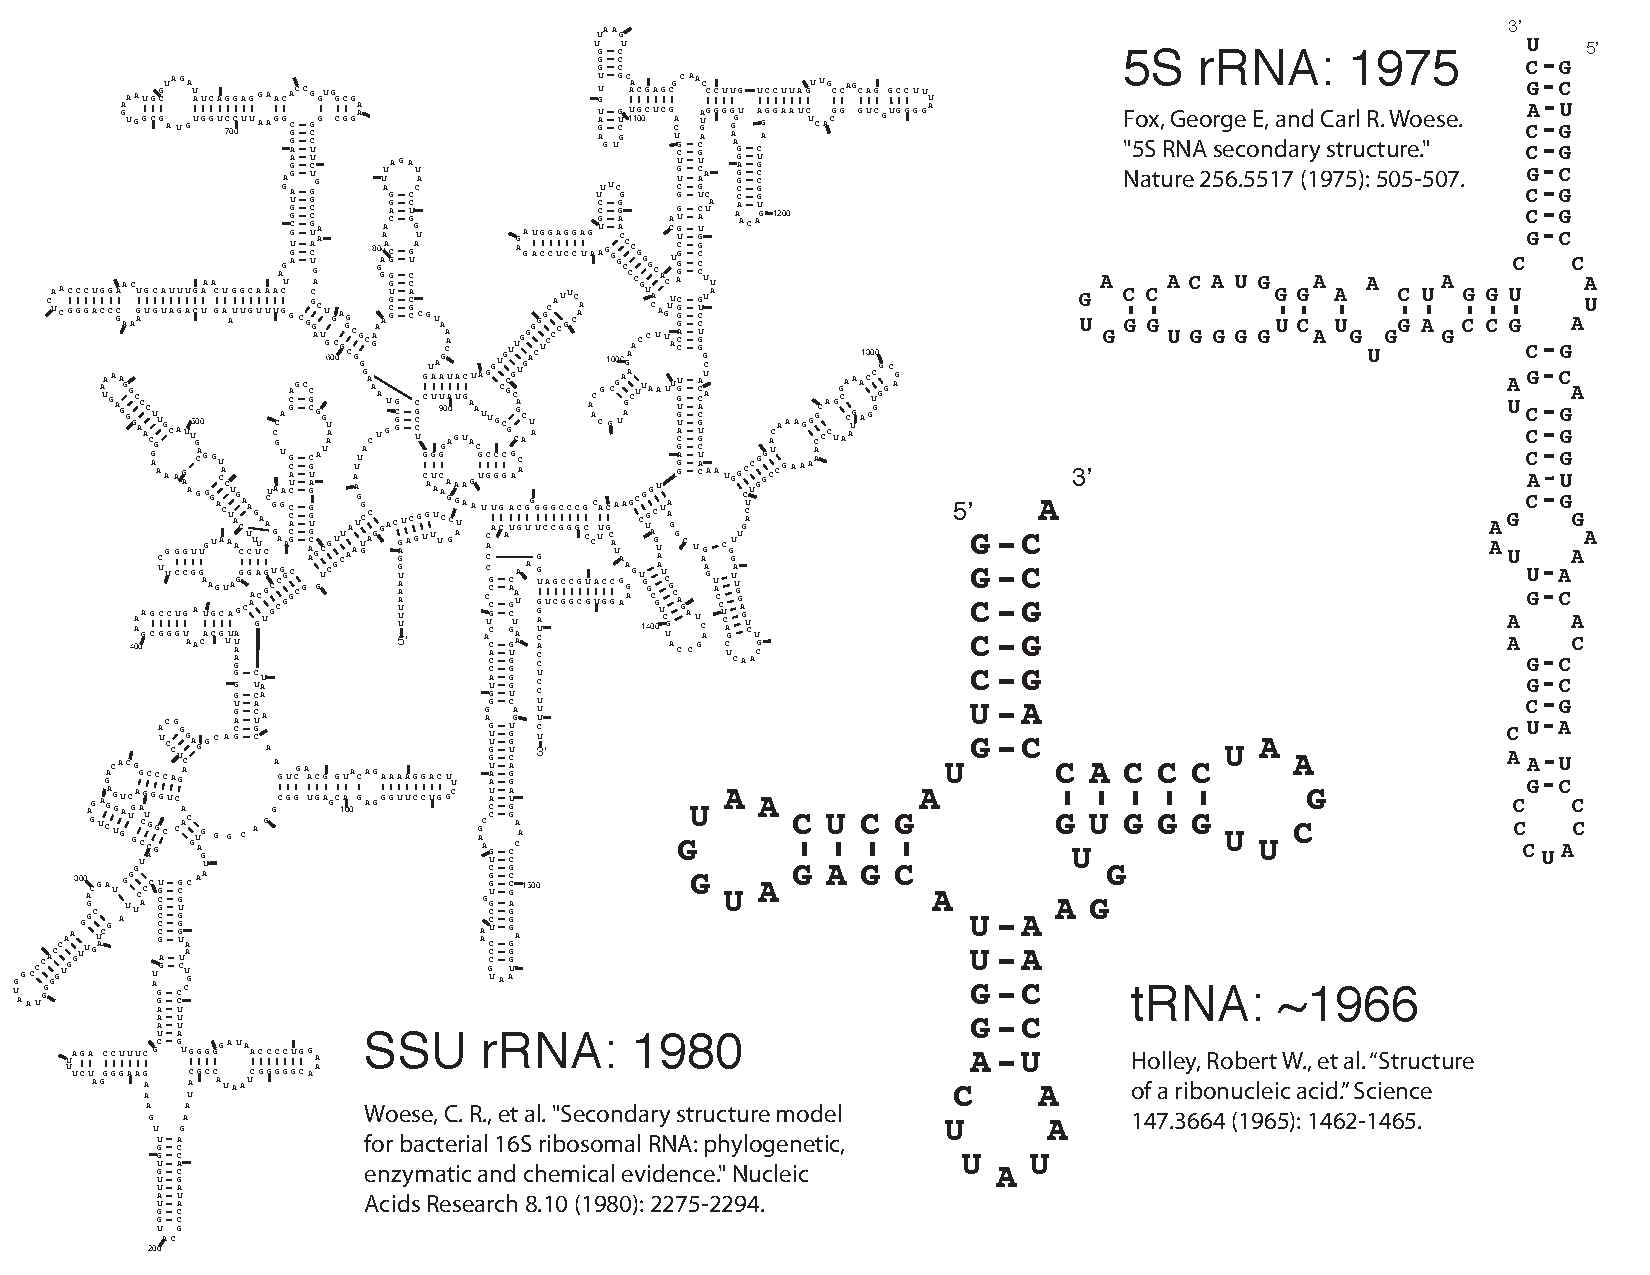
\includegraphics[width=10.5in]{figs/16s-5s-trna-allblack-dates-refs}}
%\end{slide}
%%%%%%%%%%%%%%%%%%%%%%%%%%%%%%%%%%%%%%%%%%%%%%%%%%%%%%%%%%%%%%%%%%%%
\begin{slide}
\begin{center}
\textbf{Functional RNAs play many vital roles in the cell}
\end{center}
\medskip

\small
\begin{center}
\begin{tabular}{r|l|cccc}
%\item
%  Noncoding RNA (ncRNA): all RNAs other than mRNA
 & key RNAs involved & archaea & bacteria & eukarya & viruses \\ \hline
 & \\ 
translation & ribosomal RNAs & x & x & x & \\
            & transfer RNAs  & x & x & x & \\
            & RNase P RNA    & x & x & x & \\
            & snoRNAs        & x &   & x & \\ 
            & SRP RNA        & x & x & x & \\ 
            & tmRNA          &   & x &   & \\ 
            & RNaseMRP       &   &   & x & \\ 
            &  \\ 
gene expression & riboswitches & ? & x & ? & \\
                & microRNAs &  & & x & x \\
                & 6S RNA & & x & x & \\ 
                & \\ 
splicing        & U1, U2, U4, U5, U6 & & & x & \\ 
                & \\
other           & tracrRNA       & x & x & \\
                & telomerase RNA & & & x & \\ 
                & group I introns& x & x & x & x \\
%                & Vault RNA      & & & x \\
                & sfRNAs       & & & & x \\
                & many more... & & & \\ 
\end{tabular}
\end{center}

\vfill
\end{slide}
%%%%%%%%%%%%%%%%%%%%%%%%%%%%%%%%%%%%%%%%%%%%%%%%%%%%%%%%%%%%%%%%%%%%%%
\begin{slide}
\begin{center}
\textbf{Functional RNAs play many vital roles in the cell}
\end{center}
\medskip

\small
\begin{center}
\begin{tabular}{r|l|cccc}
%\item
%  Noncoding RNA (ncRNA): all RNAs other than mRNA
 & key RNAs involved & archaea & bacteria & eukarya & viruses \\ \hline
 & \\ 
translation & ribosomal RNAs & x & x & x & \\
            & transfer RNAs  & x & x & x & \\
            & RNase P RNA    & x & x & x & \\
            & snoRNAs        & x &   & x & \\ 
            & SRP RNA        & x & x & x & \\ 
            & tmRNA          &   & x &   & \\ 
            & RNaseMRP       &   &   & x & \\ 
            &  \\ 
gene expression & riboswitches & ? & x & ? & \\
                & microRNAs &  & & x & x \\
                & 6S RNA & & x & x & \\ 
                & \\ 
splicing        & U1, U2, U4, U5, U6 & & & x & \\ 
                & \\
other           & tracrRNA       & x & x & \\
                & telomerase RNA & & & x & \\ 
                & group I introns& x & x & x & x \\
%                & Vault RNA      & & & x & \\
                & sfRNAs       & & & & x \\
                & many more... & & & & \\ 
\end{tabular}


\center{
\includegraphics[width=2.5in]{figs/rfam-logo}}

database of more than 4100 non-coding RNA families \\ each represented by a
secondary structure, alignment, and covariance model.
\end{center}

\vfill
\end{slide}
%%%%%%%%%%%%%%%%%%%%%%%%%%%%%%%%%%%%%%%%%%%%%%%%%%%%%%%%%%%%%%%%%%%%
%%%%%%%%%%%%%%%%%%%%%%%%%%%%%%%%%%%%%%%%%%%%%%%%%%%%%%%%%%%%%%
\begin{slide}
\begin{center}
{\bf Many functional RNAs adopt a conserved 3-dimensional 
  structure}
\medskip

%Three representations of a transfer RNA:

%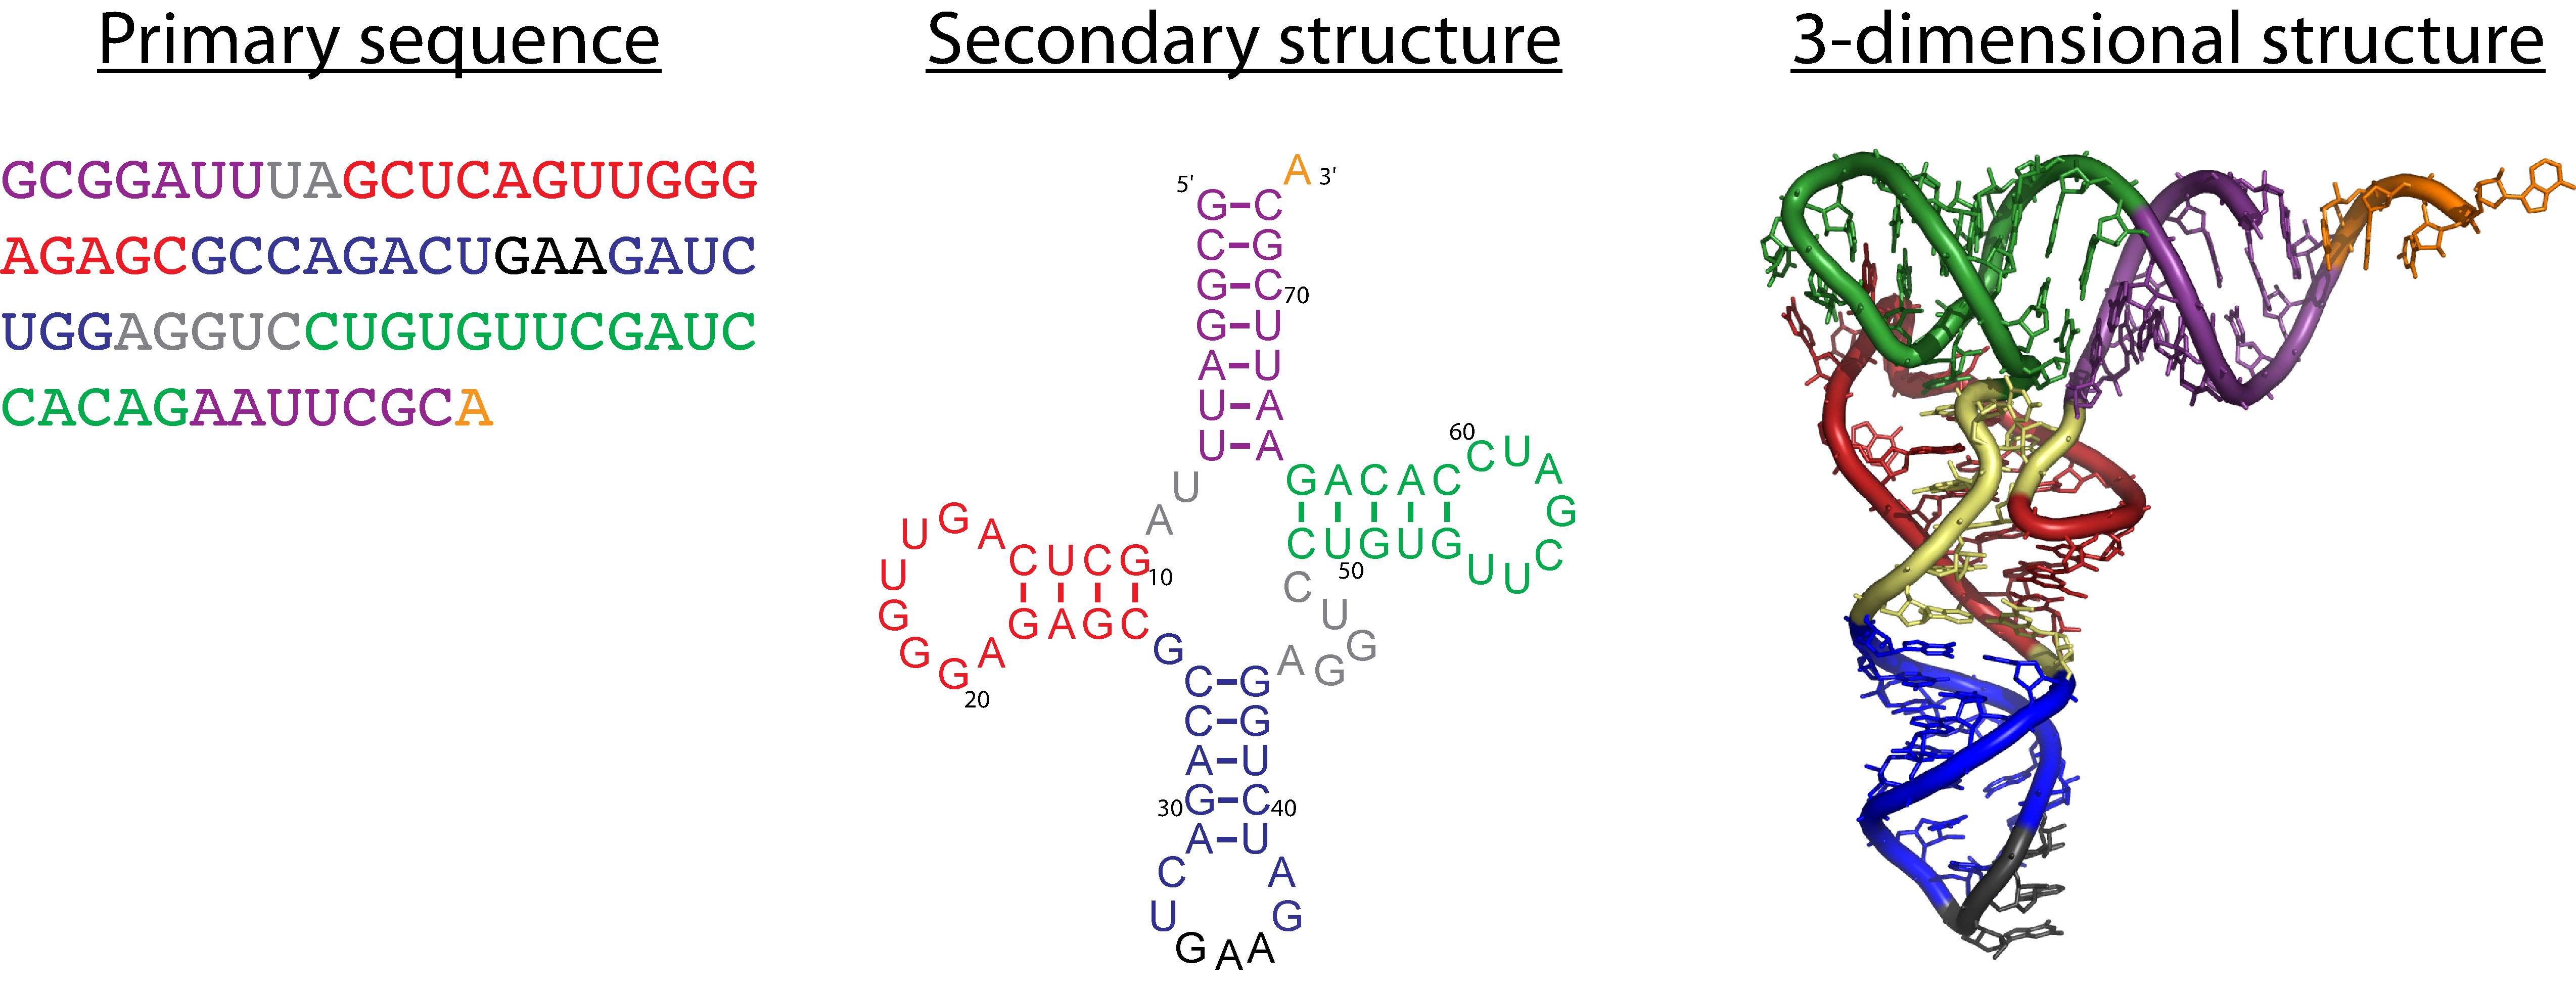
\includegraphics[width=10.5in]{figs/trna-123}
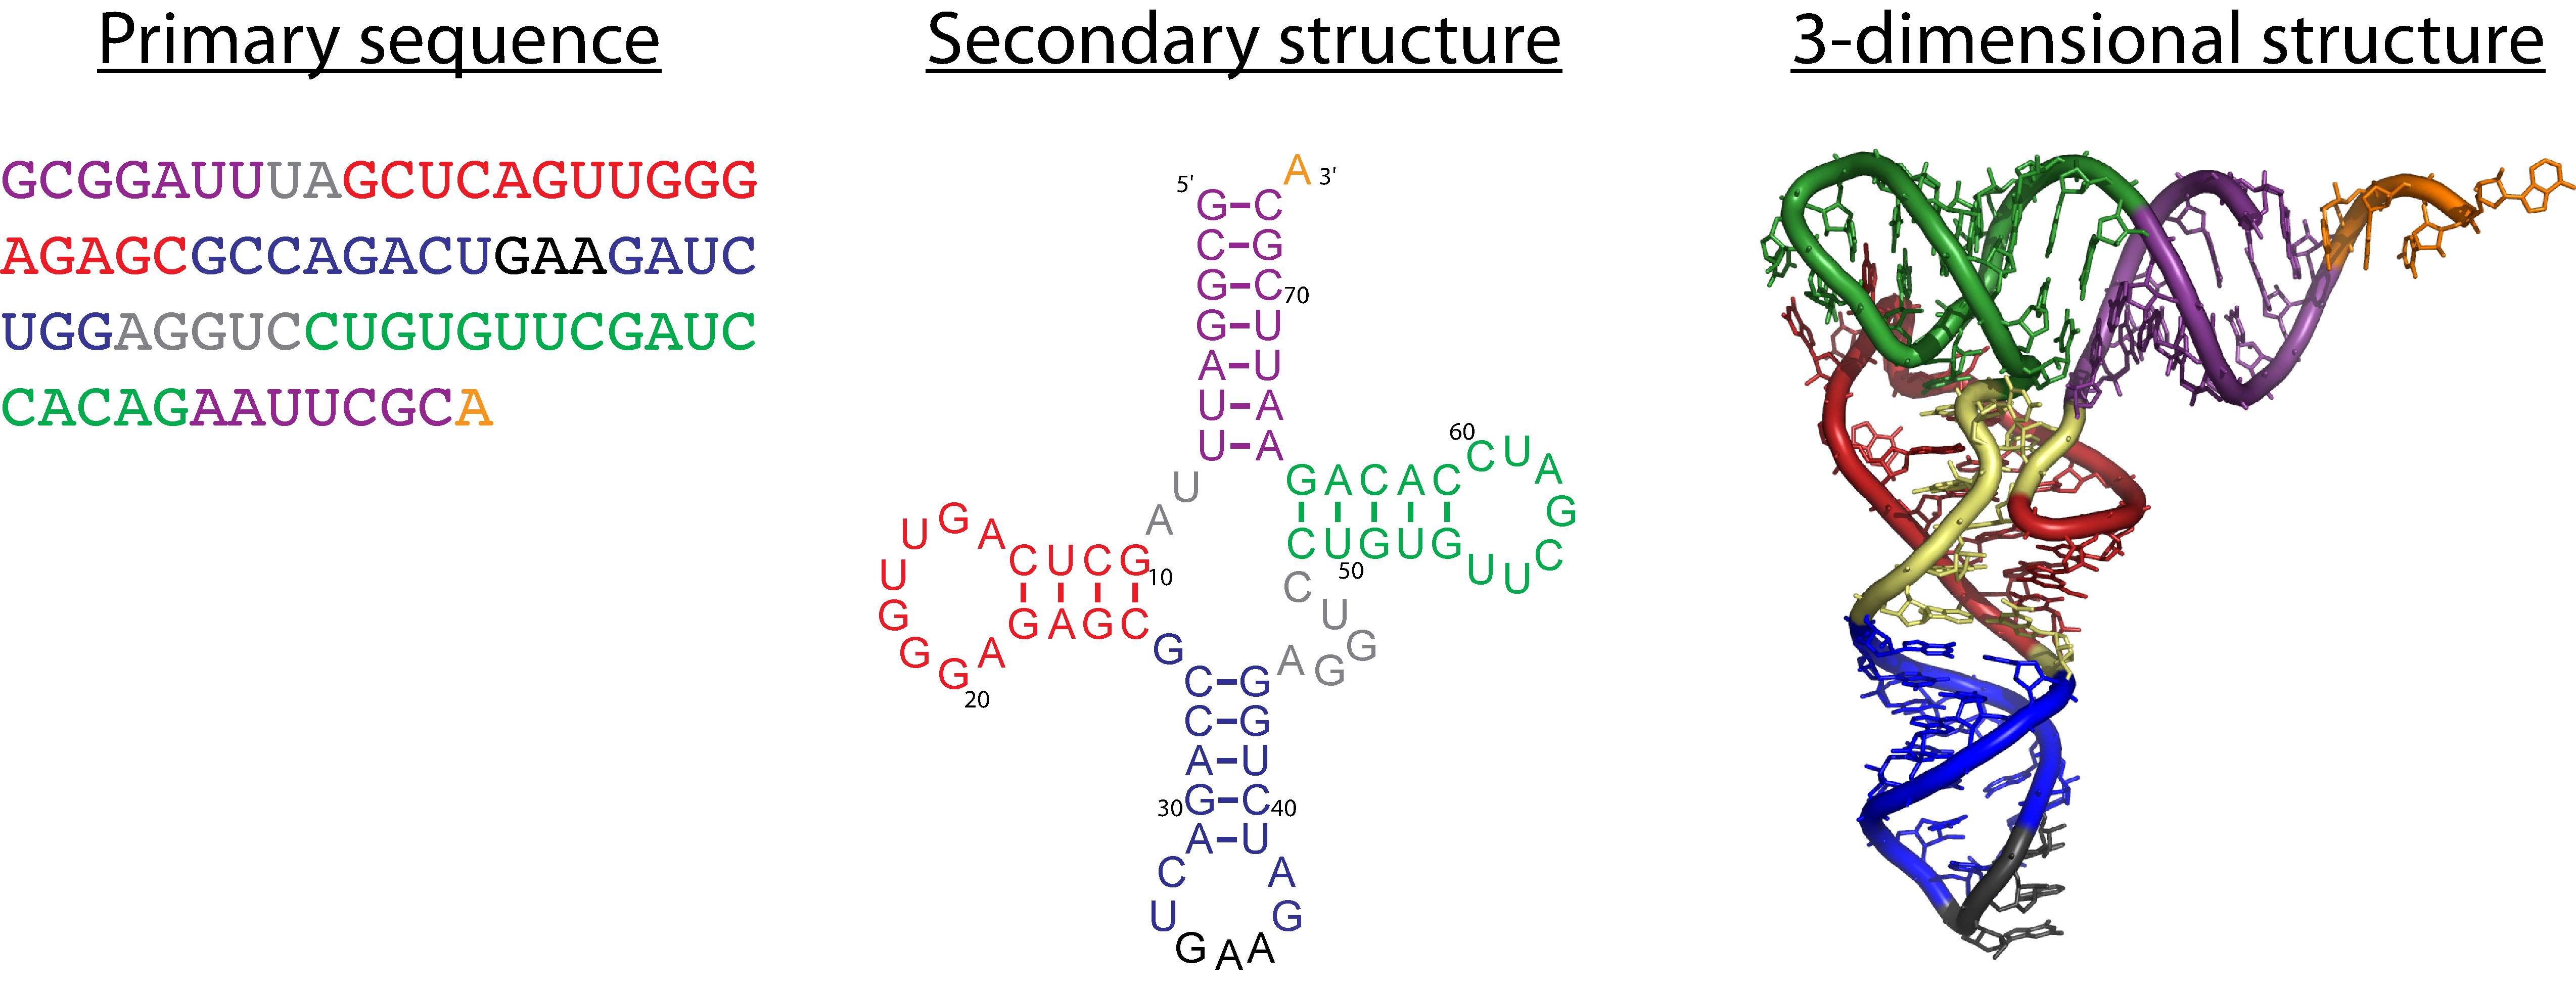
\includegraphics[width=9in]{figs/trna-123}
\end{center}

\small
\begin{itemize}
\item
  BLAST: given a single sequence, search genomes for similar sequences.
\item
  Structural RNAs are difficult to find
  \begin{itemize}
  \item short ($\sim$ 100 nt) and evolve rapidly at sequence level
  \item lack open reading frames
  \item small, 4 letter alphabet 
  \end{itemize}
  \item
  BLAST cannot take advantage of:
\begin{itemize}
  \item sequence conservation, which varies across the gene
  \item secondary structure
\end{itemize}
\end{itemize}

\vfill

\end{slide}
%%%%%%%%%%%%%%%%%%%%%%%%%%%%%%%%%%%%%%%%%%%%%%%%%%%%%%%%%%%%%
%%%%%%%%%%%%%%%%%%%%%%%%%%%%%%%%%%%%%%%%%%%%%%%%%%%%%%%%%%%%%%%%%%%%
\begin{slide}
\begin{center}
%\textbf{Comparative analysis of sequence families}: \\
\textbf{Sequence conservation provides \\ information for homology searches}

\medskip
Conservation levels vary across alignment columns.

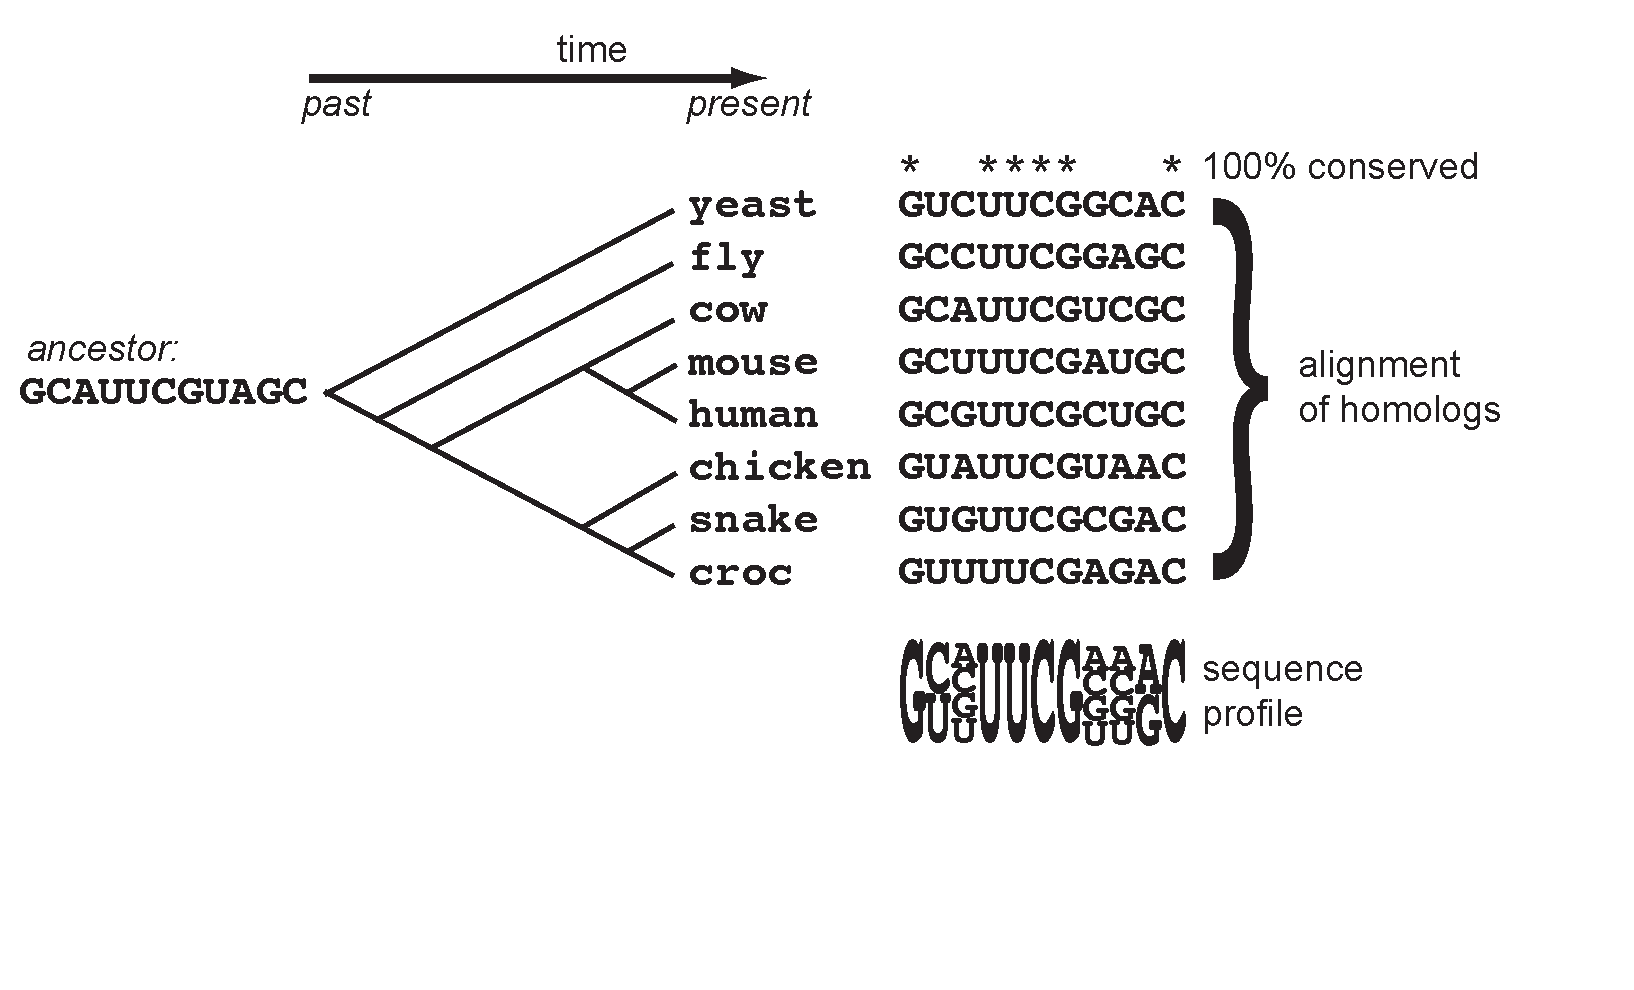
\includegraphics[width=10in]{figs/seqstructprofiles-seq1}
\end{center}

\vfill
\end{slide}
%%%%%%%%%%%%%%%%%%%%%%%%%%%%%%%%%%%%%%%%%%%%%%%%%%%%%%%%%%%%%%%%%%%%%%
\begin{slide}
\begin{center}
\textbf{Structure conservation provides additional information}
\medskip

Base-paired positions covary \\ to maintain Watson-Crick complementarity.

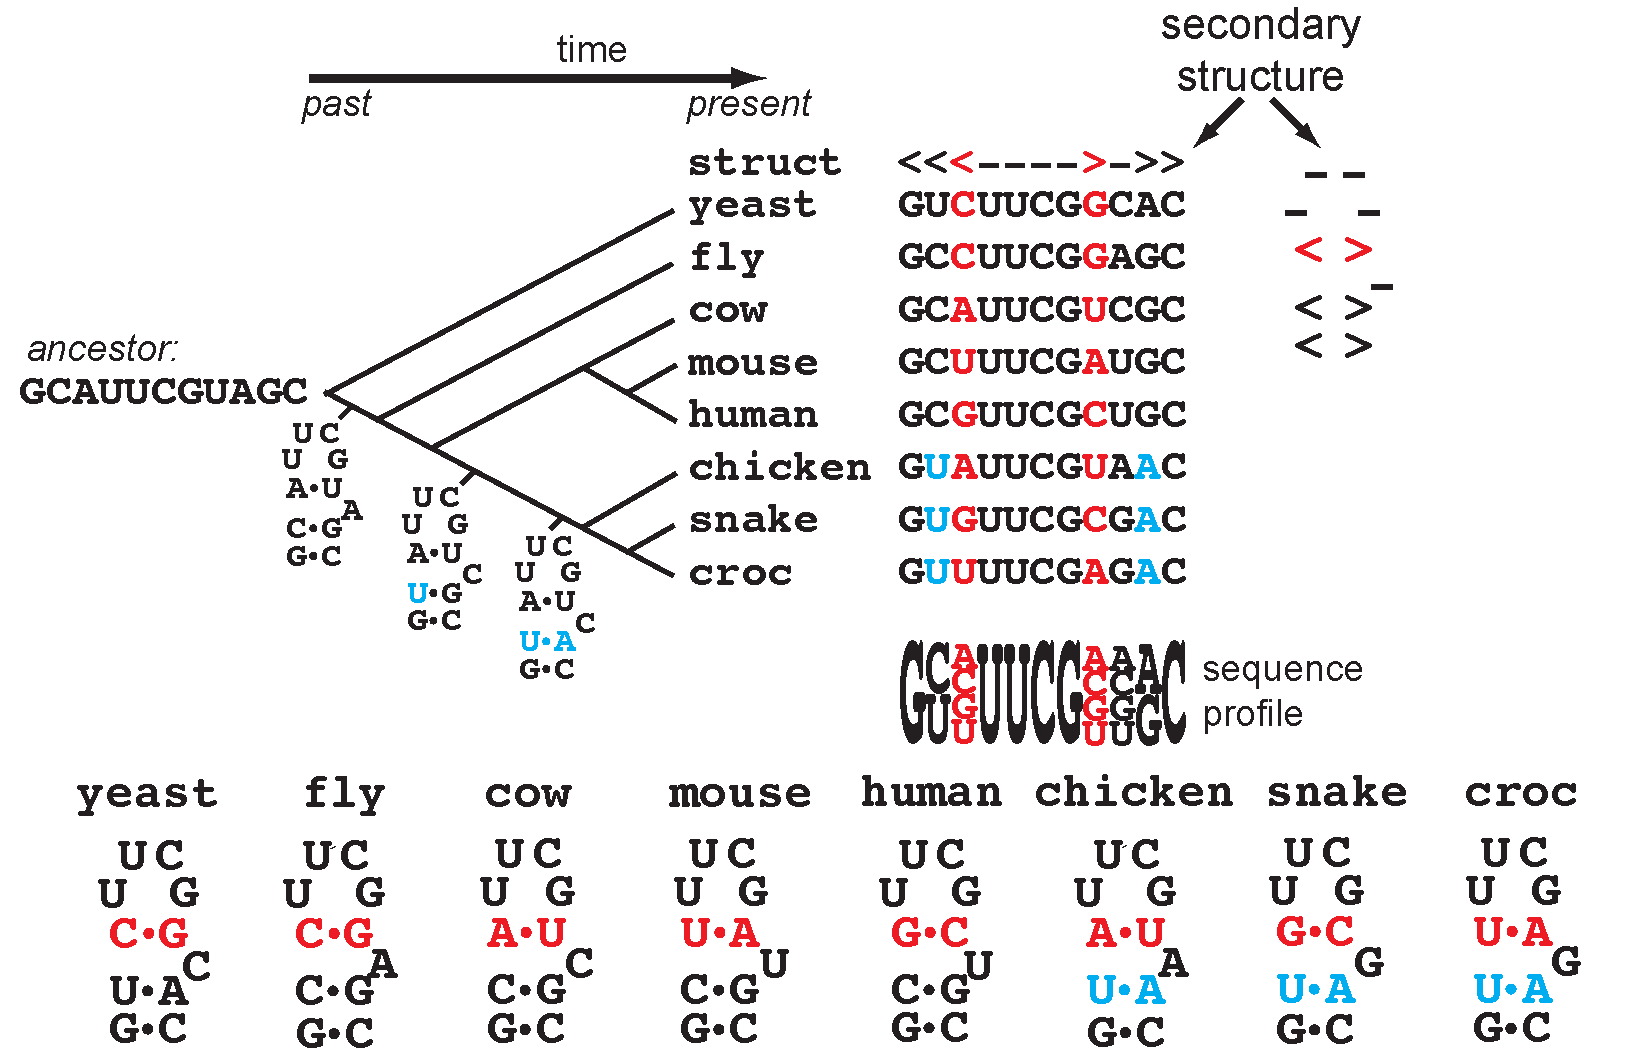
\includegraphics[width=10in]{figs/seqstructprofiles-struct2}
\end{center}

\vfill
\end{slide}
%%%%%%%%%%%%%%%%%%%%%%%%%%%%%%%%%%%%%%%%%%%%%%%%%%%%%%%%%%%%%%%%%%%%%%%%%%
%%%%%%%%%%%%%%%%%%%%%%%%%%%%%%%%%%%%%%%%%%%%%%%%%%%%%%%%%%%%%%%%%%%%%%%%%%
%xxxxxxxxxxxxxxxxxxxxxxxxxxxxxxxxxxxxxxxxxxxxxxxxxxxxxxxxxxx
\begin{comment}
\begin{slide}
\begin{center}
\textbf{Levels of sequence and structure conservation in RNA families}
\end{center}
\medskip

\begin{center}
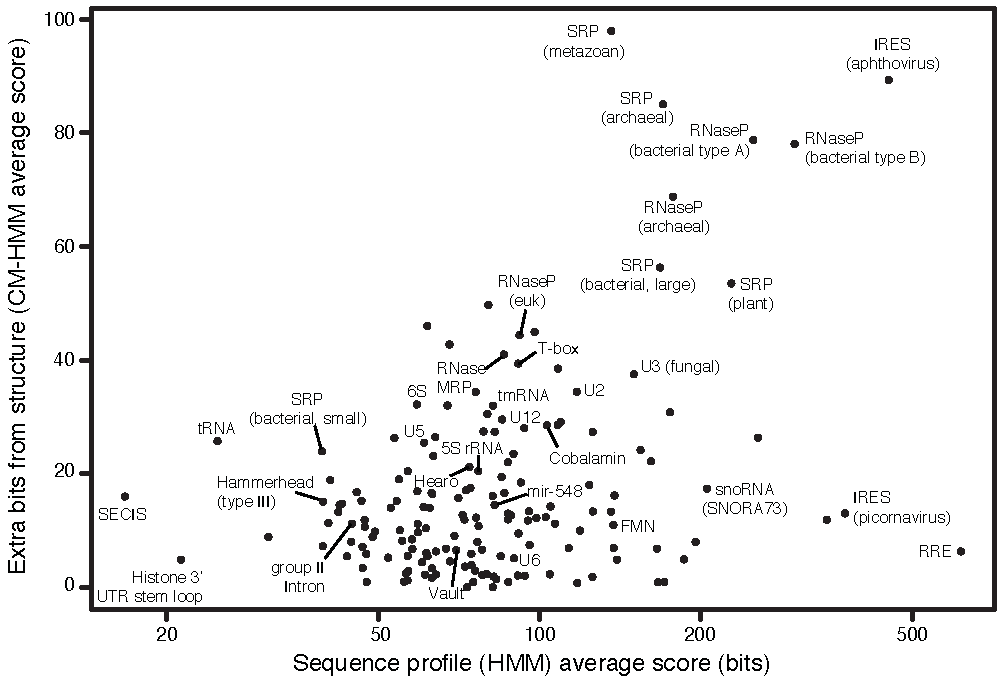
\includegraphics[height=6.5in]{figs/avgscores-rfam11}
\end{center}

\vfill

\end{slide}
\end{comment}
%xxxxxxxxxxxxxxxxxxxxxxxxxxxxxxxxxxxxxxxxxxxxxxxxxxxxxxxxxxx
%%%%%%%%%%%%%%%%%%%%%%%%%%%%%%%%%%%%%%%%%%%%%%%%%%%%%%%%%%%%%%%%%%%
\begin{slide}
\begin{center}
\textbf{profile HMMs and covariance models}
%\textbf{Eddy lab software for profile probabilistic models } (since 1994)
%\textbf{Eddy lab software for profile probabilistic models } (since 1994)
\end{center}
\medskip

\begin{center}
\small
\begin{tabular}{r|cc} 
%             &         & sequence \\
%             & sequence& and structure \\
%             & profiles& profiles \\ \hline
             & sequence & sequence and \\
             & profiles & structure profiles \\ \hline
  \\
  models     & profile HMMs     & {\color{red} covariance models (CMs)} \\ 
  \\
  software   & {\sc HMMER}      & {\sc Infernal} \\ 
  \\
  main use   & proteins,         & structural RNAs \\ 
             & repetitive DNA elements &  \\
  \\
  databases  & {\sc Pfam} and \sc{Dfam}       & {\sc Rfam} \\
             & (23794 and 4150 entries) & (4178 families) \\
  \\
%  primary sequence & yes & yes \\
%  \\
%  secondary structure & no & yes \\
%  \\
%  algorithms & Viterbi, Forward & CYK, Inside \\
%%             & Forward & Inside \\
%             &         & \\
%  complexity & $O(LN)$ & $O(LN^{2} log N)$ \\
%  \\
  performance& faster but    & slower but    \\
  for RNAs   & less accurate & more accurate \\
\end{tabular}

%\hspace{1.2in}\includegraphics[height=2in]{figs/hmmer_logo}\hspace{1.05in}\includegraphics[height=2.6in]{figs/infernal_logo}
\hspace{1.8in}
\includegraphics[height=2.7in]{figs/hmmer-infernal-refs-2019}

\end{center}

\vfill

\end{slide}
%%%%%%%%%%%%%%%%%%%%%%%%%%%%%%%%%%%%%%%%%%%%%%%%%%%%%%%%%%%%%%%%%%%%
%%%%%%%%%%%%%%%%%%%%%%%%%%%%%%%%%%%%%%%%%%%%%%%%%%%%%%%%%%%%%%%
%xxxxxxxxxxxxxxxxxxxxxxxxxxxxxxxxxxxxxxxxxxxxxxxxxxxxxxxxxxxxxx
\begin{comment}
\begin{slide}
\begin{center}
\textbf{Is the added complexity worth it? \\
  RMARK: a challenging \underline{internal} RNA homology search
  benchmark}

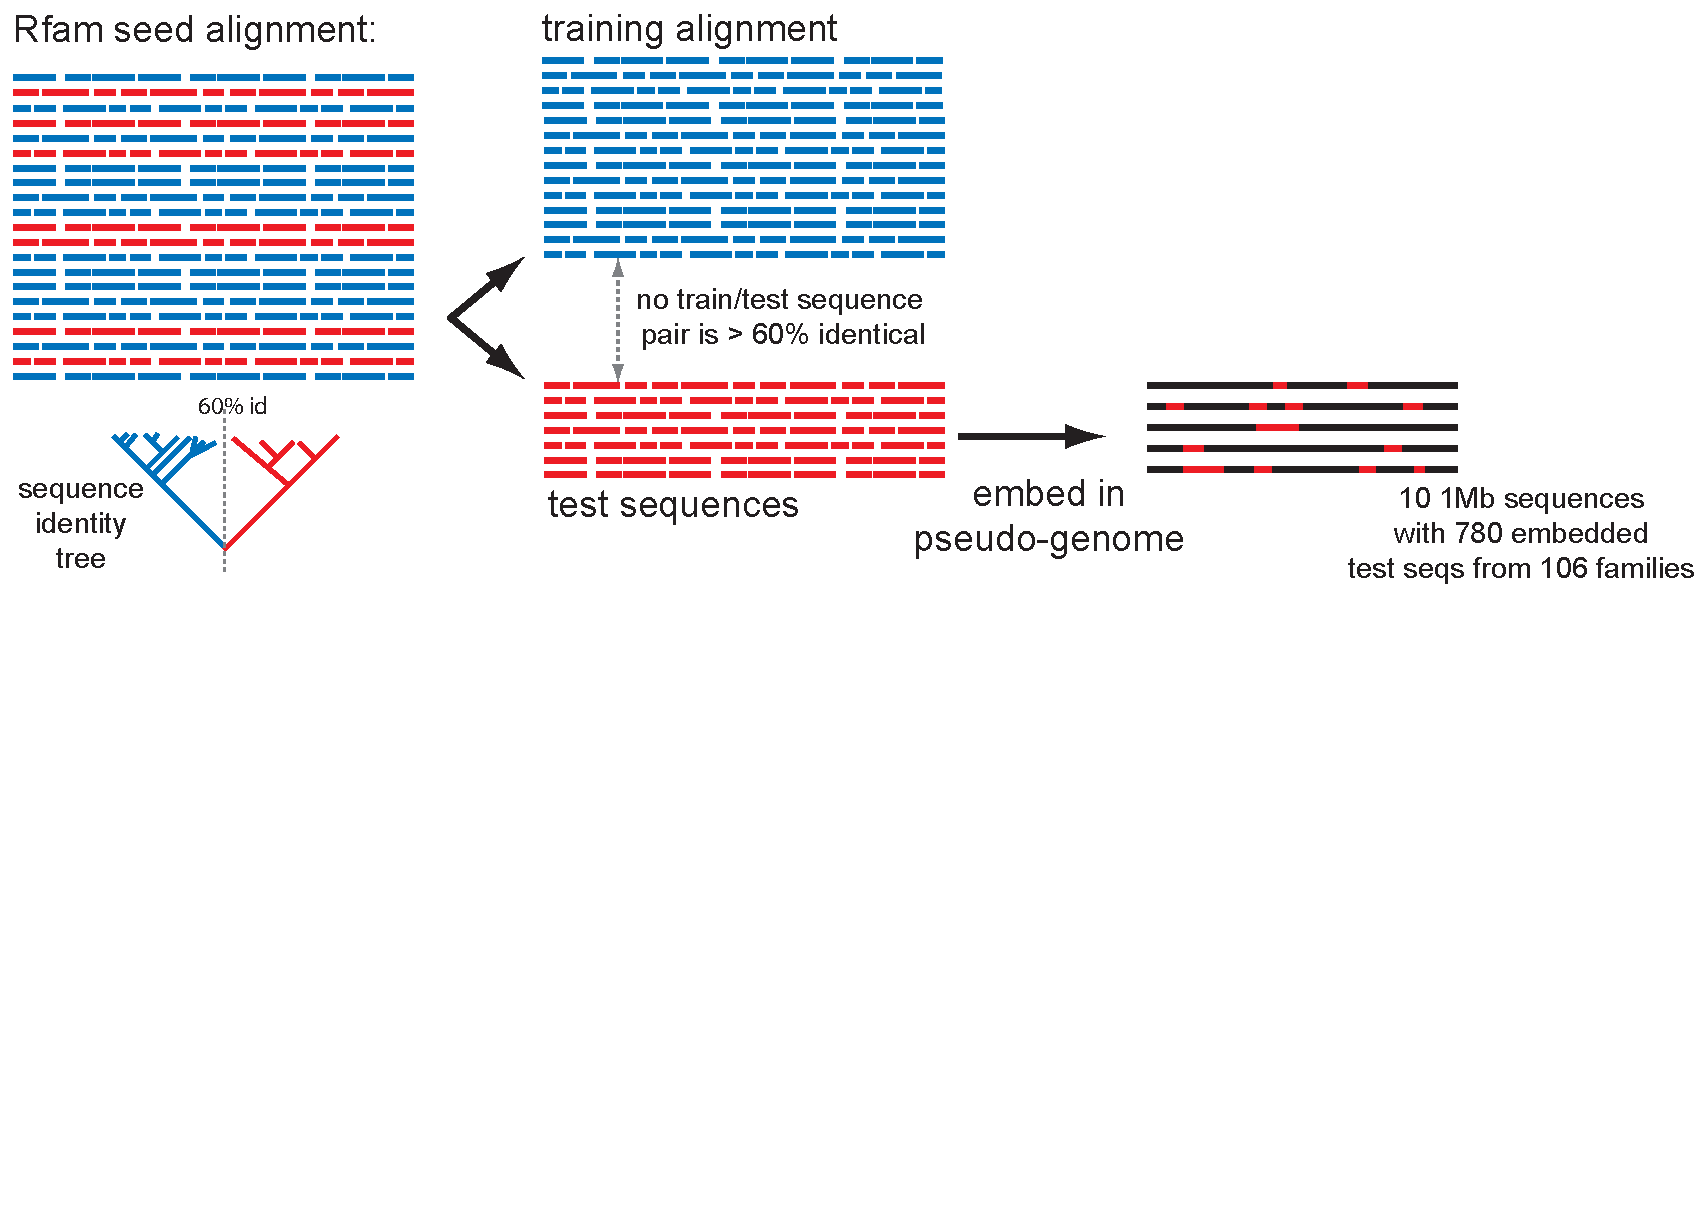
\includegraphics[width=10in]{figs/rmark-tree-1}
\end{center}

\vfill
\end{slide}
%%%%%%%%%%%%%%%%%%%%%%%%%%%%%%%%%%%%%%%%%%%%%%%%%%%%%%%%%%%%%%%%%%%%%%
\begin{slide}
\begin{center}
\textbf{Is the added complexity worth it? \\
  RMARK: a challenging \underline{internal} RNA homology search
  benchmark}

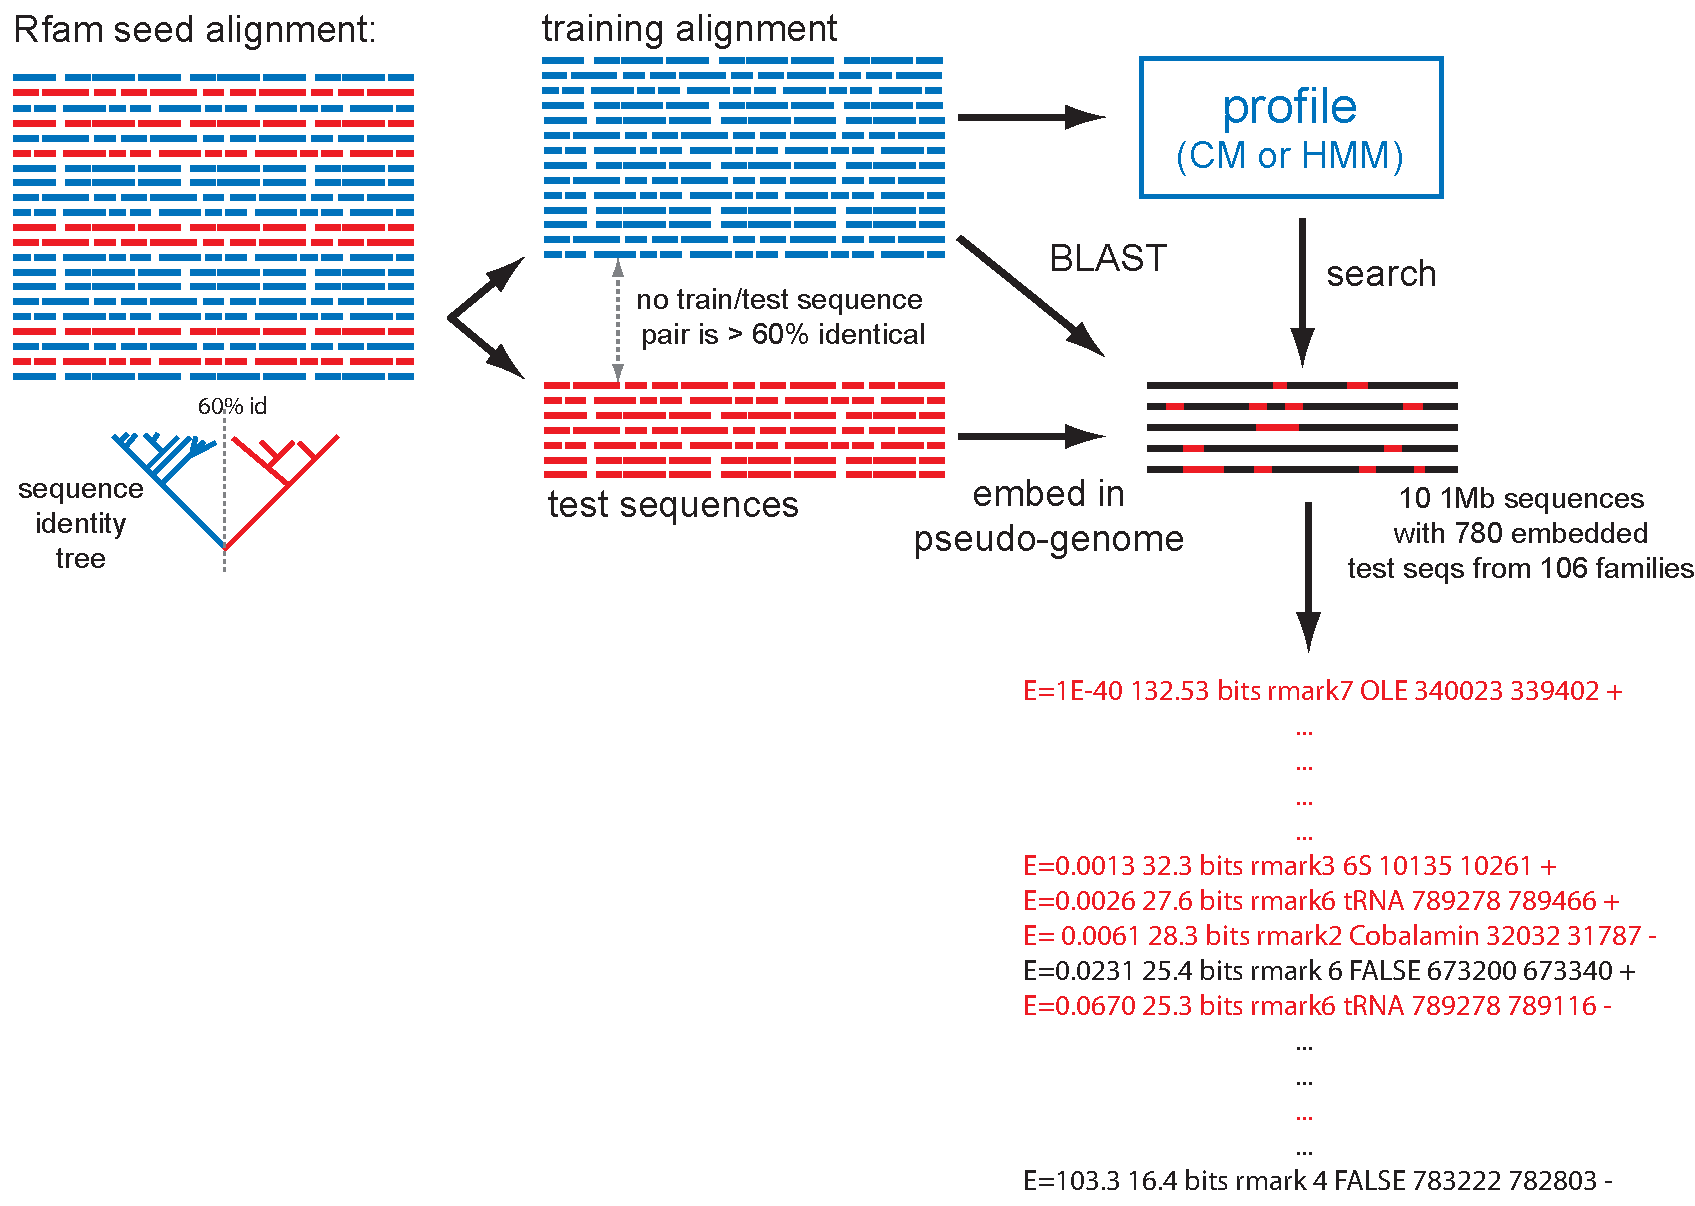
\includegraphics[width=10in]{figs/rmark-tree-2}
\end{center}

\vfill
\end{slide}
\end{comment}
%xxxxxxxxxxxxxxxxxxxxxxxxxxxxxxxxxxxxxxxxxxxxxxxxxxxxxxxxxxxxxx
%%%%%%%%%%%%%%%%%%%%%%%%%%%%%%%%%%%%%%%%%%%%%%%%%%%%%%%%%%%%%%%%%%%%%%
\begin{slide}
\begin{center}

\textbf{Infernal outperforms primary-sequence based methods on our
  benchmark (and others\footnote{Freyhult EK, Bollback JP, Gardner
    PP. Genome Res. 2007 17: 117-125.}, not shown)}

\end{center}
\medskip

\center{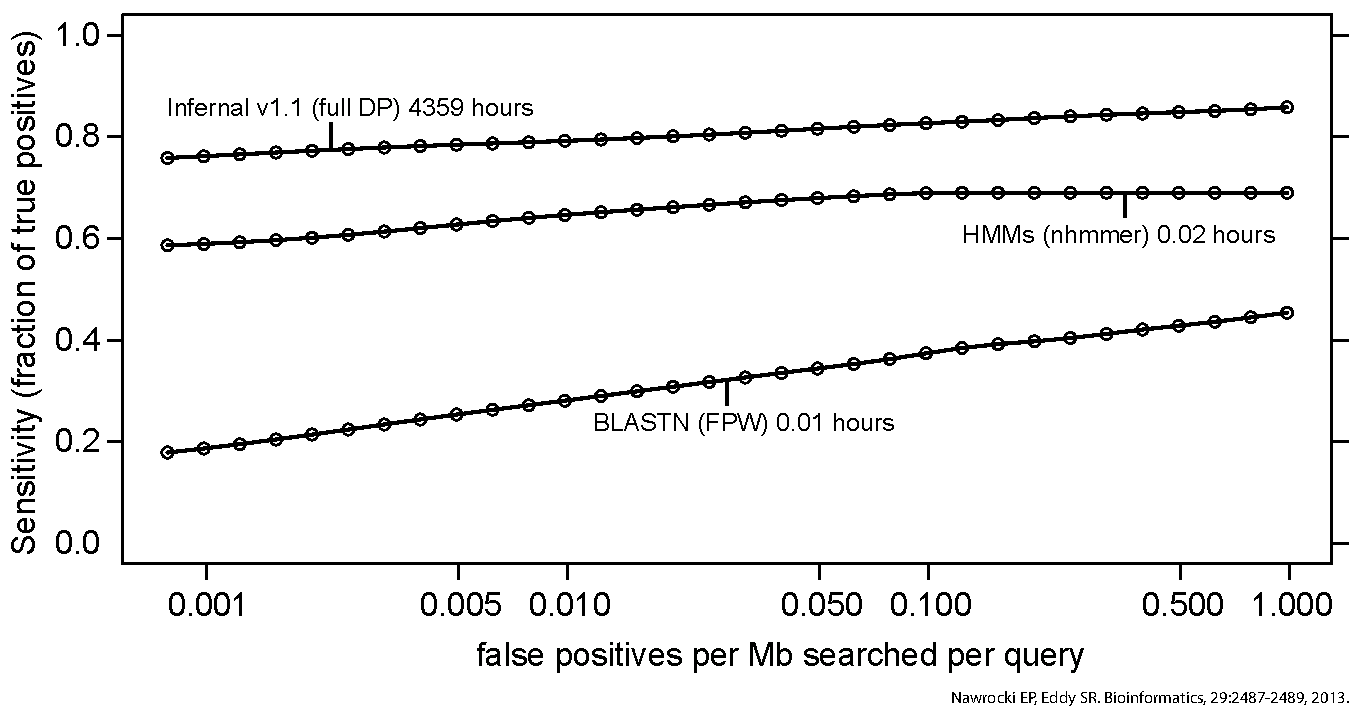
\includegraphics[width=10in]{figs/roc-talk-rcb-2014-1}}

\vfill 
\end{slide}
%%%%%%%%%%%%%%%%%%%%%%%%%%%%%%%%%%%%%%%%%%%%%%%%%%%%%%%%%%%%%%%%%%%%%%
%%%%%%%%%%%%%%%%%%%%%%%%%%%%%%%%%%%%%%%%%%%%%%%%%%%%%%%%%%%%%%%%%%%%%%
\begin{slide}
\center{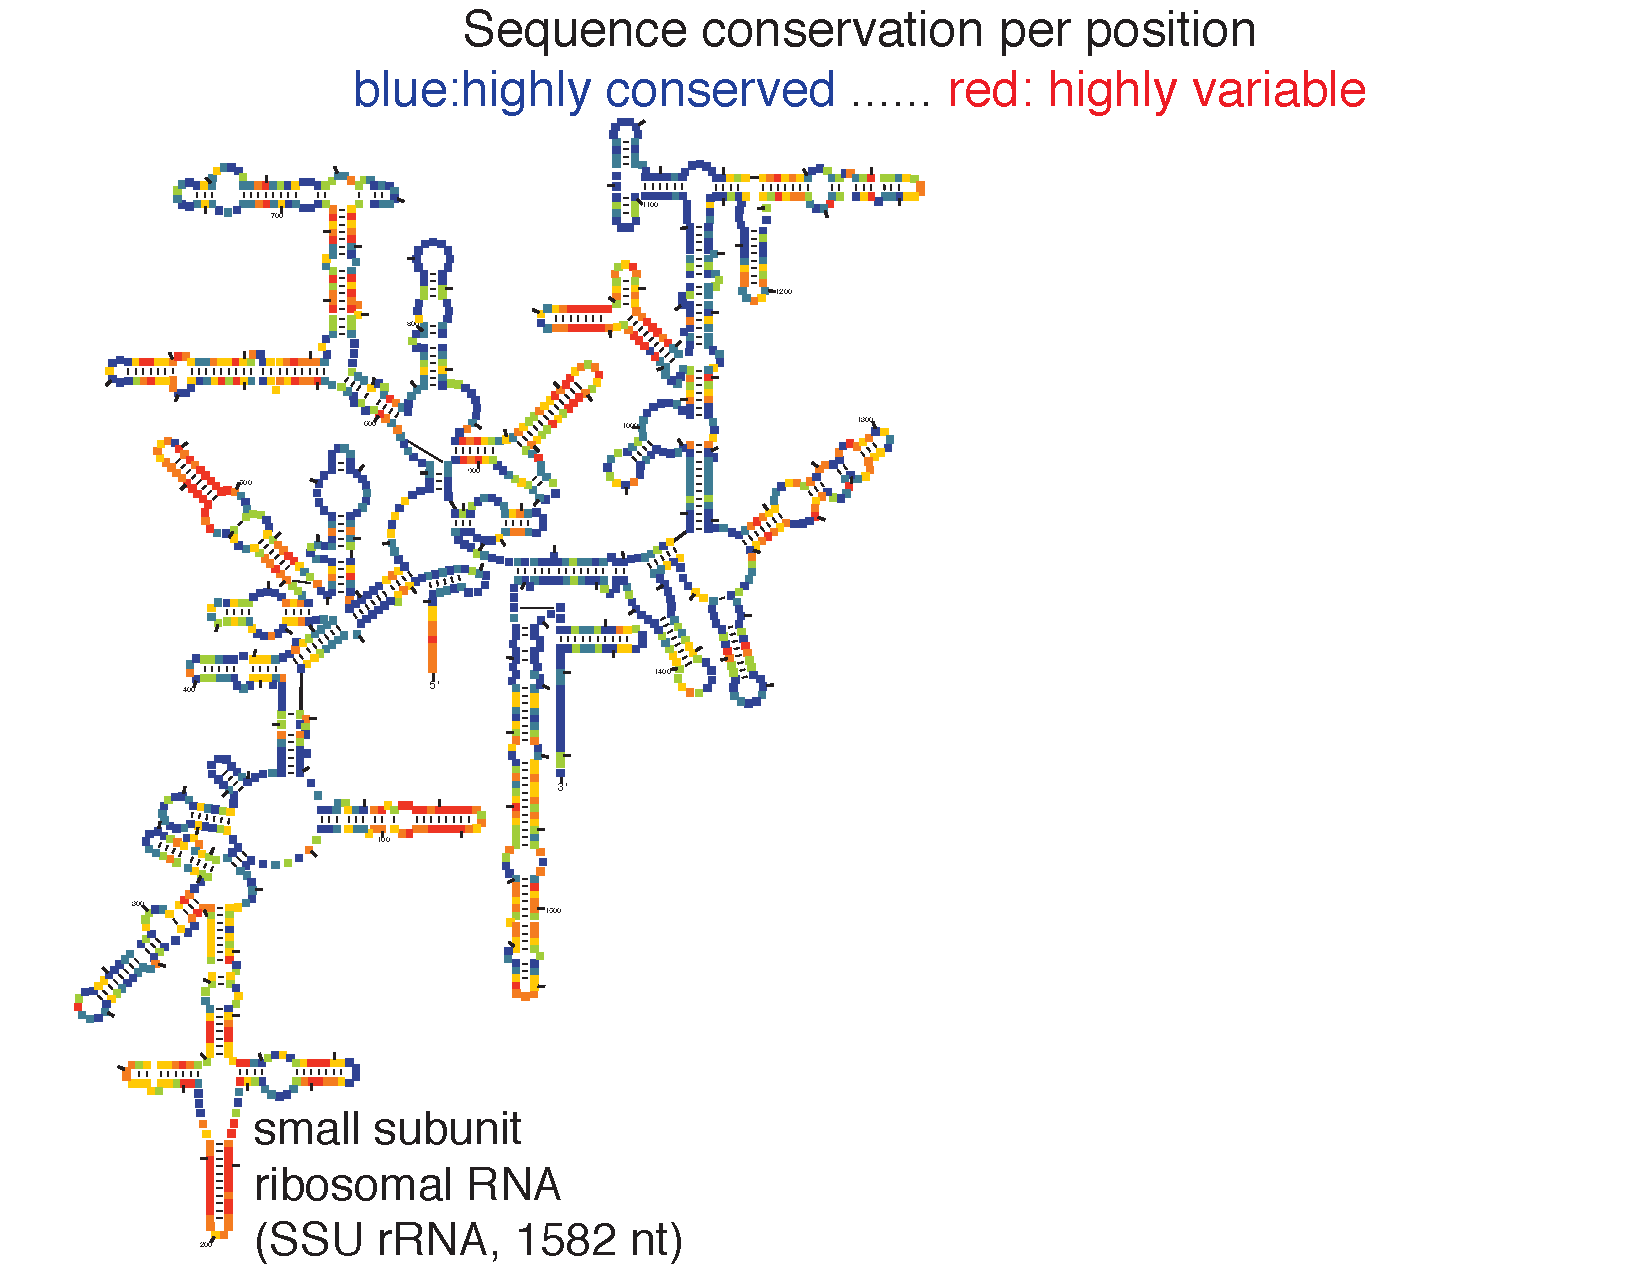
\includegraphics[width=10.5in]{figs/16s-5s-trna-info-16sonly}}
\end{slide}
%%%%%%%%%%%%%%%%%%%%%%%%%%%%%%%%%%%%%%%%%%%%%%%%%%%%%%%%%%%%%%%%%%%%%%
\begin{slide}
\center{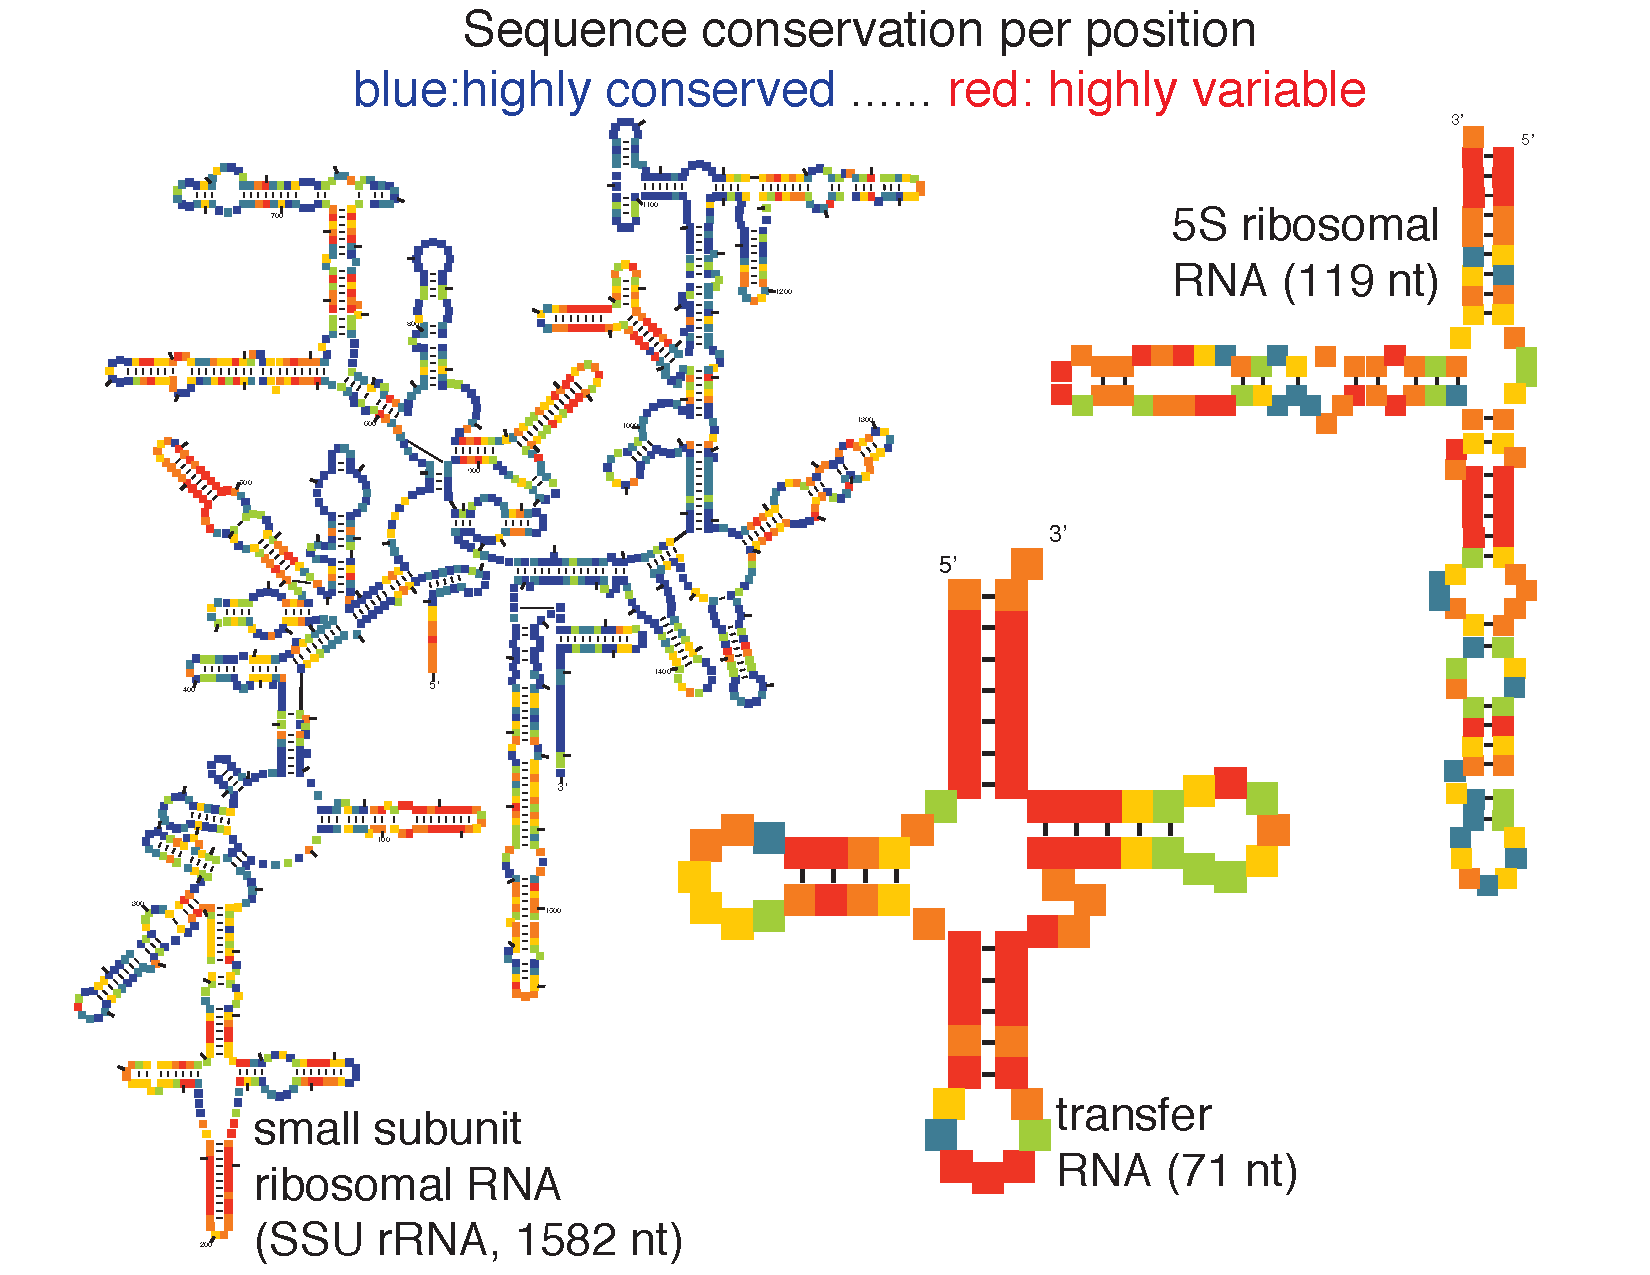
\includegraphics[width=10.5in]{figs/16s-5s-trna-info}}
\end{slide}
%%%%%%%%%%%%%%%%%%%%%%%%%%%%%%%%%%%%%%%%%%%%%%%%%%%%%%%%%%%%%%%%%%%%
%%%%%%%%%%%%%%%%%%%%%%%%%%%%%%%%%%%%%%%%%%%%%%%%%%%%%%%%%%%%%%%%%%%%%%
\begin{slide}
\begin{center}
\large
\textbf{Filter target database using profile HMMs\footnote{Weinberg,
    Ruzzo, RECOMB, 243-251, 2004; Weinberg, Ruzzo, Bioinformatics,
    22(1) 35-39 2006.}}
\end{center}

\center{\includegraphics[height=4in]{figs/filter-2014-1}}

\vfill
\end{slide}
%%%%%%%%%%%%%%%%%%%%%%%%%%%%%%%%%%%%%%%%%%%%%%%%%%%%%%%%%%%%%%%%%%%%%%%%%%
\begin{slide}
\begin{center}
\large
\textbf{Filter target database using profile HMMs\footnote{Weinberg,
    Ruzzo, RECOMB, 243-251, 2004; Weinberg, Ruzzo, Bioinformatics,
    22(1) 35-39 2006.}}
\end{center}

\center{\includegraphics[height=4in]{figs/filter-2014-1}}

\begin{itemize}
\item Even if we filter out 99\% of the database (for up to 100X
  acceleration), searches will still be too slow.
\item CM step needs to be accelerated. 
\end{itemize}

\vfill
\end{slide}
%%%%%%%%%%%%%%%%%%%%%%%%%%%%%%%%%%%%%%%%%%%%%%%%%%%%%%%%%%%%%%%%%%%%%%%%%%
%\begin{slide}
%\begin{center}
%
%\textbf{Accelerating CM alignment step 1: \\ align sequence with HMM}
%
%\includegraphics[height=6in]{figs/hmm_alignment2_layer2}
%\end{center}
%
%\vfill
%\end{slide}
%%%%%%%%%%%%%%%%%%%%%%%%%%%%%%%%%%%%%
%%%%%%%%%%%%%%%%%%%%%%%%%%%%%%%%%%%%%%%%%%%%%%%%%%%%%%%%%%%%%%%%%%%%%%%%%%
\begin{slide}
\begin{center}

%\textbf{Accelerating CM alignment step 2: \\ HMM posterior decoding to
%  get confidence estimates}
\textbf{Accelerating CM alignment step 1: \\ HMM posterior decoding to
  get confidence estimates}

\includegraphics[height=6in]{figs/hmm_alignment2_layer3}
\end{center}

\vfill
\end{slide}
%%%%%%%%%%%%%%%%%%%%%%%%%%%%%%%%%%%%%
\begin{slide}
\begin{center}

%\textbf{Accelerating CM alignment step 2: \\ use HMM alignment
%  confidence to constrain CM alignment\footnote{M. P. Brown. Proc. Int. Conf. ISMB, 8:57–66, 2000.}}
\textbf{Accelerating CM alignment step 2: \\ use HMM alignment
  confidence to constrain CM alignment}
\end{center}
\medskip
\small
%\begin{itemize}
%\item
%\textbf{main idea:} eliminate potential alignments the HMM tells us are very improbable
%\end{itemize}
\begin{center}
\includegraphics[width=8in]{figs/post_hmm_to_cm_map2_layer14}
\end{center}
\vfill
\end{slide}
%%%%%%%%%%%%%%%%%%%%%%%%%%%%%%%%%%%%%%%%%%%%%%%%%%%%%%%%%%%%%%%%%%%%%%
\begin{slide}
\begin{center}

%\textbf{Accelerating CM alignment step 2: \\ use HMM alignment
%  confidence to constrain CM alignment\footnote{M. P. Brown. Proc. Int. Conf. ISMB, 8:57–66, 2000.}}
\textbf{Accelerating CM alignment step 2: \\ use HMM alignment
  confidence to constrain CM alignment}
\end{center}
\medskip
\small
%\begin{itemize}
%\item
%\textbf{main idea:} eliminate potential alignments the HMM tells us are very improbable
%\end{itemize}
\begin{center}
\includegraphics[width=8in]{figs/post_hmm_to_cm_map2_layer15}
\end{center}
\vfill
\end{slide}
%%%%%%%%%%%%%%%%%%%%%%%%%%%%%%%%%%%%%%%%%%%%%%%%%%%%%%%%%%%%%%%%%%%%%%%%%%
\begin{slide}
\begin{center}

%\textbf{Accelerating CM alignment step 3: \\ use HMM alignment
%  confidence to constrain CM alignment\footnote{M. P. Brown. Proc. Int. Conf. ISMB, 8:57–66, 2000.}}
\textbf{Accelerating CM alignment step 3: \\ use HMM alignment
  confidence to constrain CM alignment}
\end{center}
\medskip
\small
%\begin{itemize}
%\item
%\textbf{main idea:} eliminate potential alignments the HMM tells us are very improbable
%\end{itemize}
\begin{center}
\includegraphics[width=8in]{figs/post_hmm_to_cm_map2_layer16}
\end{center}
\vfill
\end{slide}
%%%%%%%%%%%%%%%%%%%%%%%%%%%%%%%%%%%%%%%%%%%%%%%%%%%%%%%%%%%%%%%%%%%%%%
\begin{slide}
\center{\includegraphics[width=10.5in]{figs/16s-5s-trna-info-16sonly}}
\end{slide}
%%%%%%%%%%%%%%%%%%%%%%%%%%%%%%%%%%%%%%%%%%%%%%%%%%%%%%%%%%%%%%%%%%%%%%
\begin{slide}
\center{\includegraphics[width=10.5in]{figs/16s-5s-trna-info}}
\end{slide}
%%%%%%%%%%%%%%%%%%%%%%%%%%%%%%%%%%%%%%%%%%%%%%%%%%%%%%%%%%%%%%%%%%%%
\begin{slide}
\begin{center}
\large
\textbf{Use HMMs as filters and to constrain CM alignment}
\end{center}

\center{\includegraphics[height=5in]{figs/filter-2014-2}}

\vfill
\end{slide}
%%%%%%%%%%%%%%%%%%%%%%%%%%%%%%%%%%%%%%%%%%%%%%%%%%%%%%%%%%%%%%%%%%%%%%%%%%
\begin{slide}
\begin{center}

\textbf{HMM-based acceleration makes Infernal 10,000 times faster}

\end{center}
\medskip

\center{\includegraphics[width=10in]{figs/roc-talk-rcb-2014-2}}

\vfill 
\end{slide}


%%%%%%%%%%%%%%%%%%%%%%%%%%%%%%%%%%%%%%%%%%%%%%%%%%%%%%%%%%%%%%%%%%%%%%
\begin{slide}
\begin{center}
\textbf{Practical structural RNA genome annotation}
\end{center}

\begin{itemize}
  \item Faster Infernal integrated into:
    \begin {itemize}
    \item
      NCBI prokaryotic genome annotation pipeline PGAP (Azat Badretdin)
    \item
      NCBI eukaryotic genome annotation (Fran\c{c}oise Thibaud-Nissen)
    \end{itemize}
\end{itemize}    

\medskip

\center{\includegraphics[width=10in]{figs/paper-pgap}}
\vfill
\end{slide}
%%%%%%%%%%%%%%%%%%%%%%%%%%%%%%%%%%%%%%%%%%%%%%%%%%%%%%%%%%%%%%%%%%%%%%
\begin{slide}

\center{\includegraphics[width=9in]{figs/paper-introns}}

\center{\includegraphics[width=7in]{figs/gp1-fig2-ss}}
% T. A. Jones, and S. R. Eddy, NAR, 2018, gky414}

\vfill
\end{slide}
%%%%%%%%%%%%%%%%%%%%%%%%%%%%%%%%%%%%%%%%%%%%%%%%%%%%%%%%%%%%%%%%%%%%%%%%
\begin{slide}
\begin{center}
\large{\textbf{GenBank indexers handle incoming sequence submissions}}
\end{center}

\center{\includegraphics[width=9in]{figs/spheres-submission-schematic-1}}

\vfill
\end{slide}

%%%%%%%%%%%%%%%%%%%%%%%%%%%%%%%%%%%%%%%%%%%%%%%%%%%%%%%%%%%%%%%%%%%%%%
\begin{slide}
\begin{center}
\textbf{Ribosensor: a tool for evaluating ribosomal RNA datasets \\ using
profiles and BLAST\footnote{Alejandro Sch\"{a}ffer developed the BLAST-based scheme}}
\end{center}

\center{\includegraphics[width=10in]{figs/ribosensor-schematic}}

\small
\begin{itemize}
\item Profile-based analysis:
\begin{itemize}
\item 18 ribosomal RNA models (15 SSU rRNA, 3 LSU rRNA); 8 from Rfam
%\item Fast first pass to classify each sequence to best-scoring model
%\item Slower second pass to align each sequence to best model and analyze the alignment
\item Detects unexpected features (``UnacceptableModel'', ``DuplicatedRegions'', etc.)
\end{itemize}
%\item BLAST-based analysis (with $\sim$15X smaller DB) that indexers are familiar with.

\item Profile and BLAST results considered together to determine PASS/FAIL
%\item About 8X faster\footnote{when tested in 2016} than previous BLAST-only approach
%\item In use for ``TLS'' submissions ($>$2500 seqs) of 16S since 2017
%\item Useful for many types of ribosomal RNAs (given models)
\end{itemize}


\vfill
\end{slide}
%%%%%%%%%%%%%%%%%%%%%%%%%%%%%%%%%%%%%%%%%%%%%%%%%%%%%%%%%%%%%%%%%%%%%%
\begin{slide}
\center{\includegraphics[height=2.5in]{figs/paper-ribovore}}

\center{\includegraphics[height=5.5in]{figs/ribovore}}

  \vfill
\end{slide}
%%%%%%%%%%%%%%%%%%%%%%%%%%%%%%%%%%%%%%%%%%%%%%%%%%%%%%%%%%%%%%%%%%%%%%
\begin{slide}
\center{\includegraphics[width=10in]{figs/paper-rfam-2024}}

  \vfill
\end{slide}
%%%%%%%%%%%%%%%%%%%%%%%%%%%%%%%%%%%%%%%%%%%%%%%%%%%%%%%%%%%%%%%%%%%%%%
\begin{slide}
\center{\includegraphics[width=10in]{figs/paper-rnacentral-2019}}

\center{\includegraphics[width=10in]{figs/paper-rnacentral-2021}}

  \vfill
\end{slide}
%%%%%%%%%%%%%%%%%%%%%%%%%%%%%%%%%%%%%%%%%%%%%%%%%%%%%%%%%%%%%%%%%%%%%%
\begin{slide}
\center{\includegraphics[width=10in]{figs/paper-r2dt-2021}}

  \vfill
\end{slide}
%%%%%%%%%%%%%%%%%%%%%%%%%%%%%%%%%%%%%%%%%%%%%%%%%%%%%%%%%%%%%%%%%%%%%%
\begin{slide}
\center{\includegraphics[width=9in]{figs/paper-r2dt-structures}}

  \vfill
\end{slide}
%%%%%%%%%%%%%%%%%%%%%%%%%%%%%%%%%%%%%%%%%%%%%%%%%%%%%%%%%%%%%%%%%%%%%%
\begin{slide}
\center{\includegraphics[width=4.5in]{figs/paper-hydractinia-2024}}

\center{\includegraphics[width=10in]{figs/rrna-gff}}

\center{\includegraphics[width=10in]{figs/trna-gff}}

  \vfill
\end{slide}
%%%%%%%%%%%%%%%%%%%%%%%%%%%%%%%%%%%%%%%%%%%%%%%%%%%%%%%%%%%%%%%%%%%%%%
\begin{slide}
\center{\includegraphics[width=10in]{figs/paper-tmrna-2025}}

\center{\includegraphics[width=10in]{figs/tmrna-templates}}

  \vfill
\end{slide}
%%%%%%%%%%%%%%%%%%%%%%%%%%%%%%%%%%%%%%%%%%%%%%%%%%%%%%%%%%%%%%%%%%%%%%
%%%%%%%%%%%%%%%%%%%%%%%%%%%%%%%%%%%%%%%%%%%%%%%%%%%%%%%%%%%%%%%%%%%%%%
\begin{slide}
\begin{center}
  \textbf{Future directions for structural RNA research}
\end{center}

  \begin{itemize}
  \item Further development of Infernal
    \begin{itemize}
    \item iterative search
    \item meta-models for clade-specific scoring
    \end{itemize}
  \item Structural RNA annotation
    \begin{itemize}
    \item group I introns: improved covariance models for Rfam
    \item viral structural RNA annotations by VADR
    \end{itemize}
  \end{itemize}    
    
  \vfill

\end{slide}
%%%%%%%%%%%%%%%%%%%%%%%%%%%%%%%%%%%%%%%%%%%%%%%%%%%%%%%%%%%%%%%%%%%%%%
\begin{slide}

\large
\begin{center}
\large{\textbf{Acknowledgements}} \\

\normalsize
\vspace{0.75in}

\small
\begin{tabular}{l|l|l}
%                  & \\ \hline
%                  & \\
\textbf{NLM - VADR}      & \textbf{NLM - Ribovore}   & \textbf{NLM - RNA annotation} \\
Alejandro Sch\"{a}ffer   & Alejandro Sch\"{a}ffer    &  Fran\c{c}oise Thibaud-Nissen \\
Rodney Brister           & Ilene Mizrachi            &  Azat Badretdin \\
Ilene Mizrachi           & Rich McVeigh              &  Terence Murphy \\
Eneida Hatcher           & Anji Johnston             &  Michael DiCuccio \\
Linda Yankie             & Beverly Underwood         &  Tatiana Tatusova \\
Vince Calhoun            & Alex Kotliarov            &  Mark Borodovsky \\
Susan Schafer            & Barbara Robbertse \\
EB Dickinson             & Conrad Schoch \\
& & \\ \hline
 & & \\    
\textbf{Harvard/Janelia} & \textbf{Rfam/RNAcentral} & \textbf{NLM - leadership} \\
Sean Eddy                &  Anton Petrov            & David Landsman \\
Tom Jones                &  Blake Sweeney           & Richard Scheuermann  \\
Diana Kolbe              &  Nancy Ontiveros         & Steve Sherry \\
Travis Wheeler           &  Kelly Williams          & Kim Pruitt  \\
Elena Rivas              &  Sam Griffith-Jones      & Jim Ostell \\
Michael Farrar           &  Paul Gardner            & David Lipman \\
\end{tabular}

\includegraphics[width=2.5in]{figs/NIH_NLM_ABRV_2C_4-white}
\includegraphics[width=2.5in]{figs/nlm-buildings}

\end{center}

\vfill

\end{slide}
%%%%%%%%%%%%%%%%%%%%%%%%%%%%%%%%%%%%%%%%%%%%%%%%%%%%%%%%%%%%%%%%%%%%%%
\begin{slide}
\begin{center}
%\textbf{profile HMMs and covariance models}
\textbf{Profile HMMs: sequence family models built from alignments}
\end{center}

\center{\includegraphics[height=6.625in]{figs/hmm}}

%An HMM generates ``homologous'' sequences.

\end{slide}
%%%%%%%%%%%%%%%%%%%%%%%%%%%%%%%%%%%%%%%%%%%%%%%%%%%%%%%%%%%%%%%
\begin{slide}
\begin{center}
%\textbf{profile HMMs and covariance models}
\textbf{Profile HMMs: sequence family models built from alignments}
\end{center}

\center{\includegraphics[height=6.625in]{figs/hmm-given}}
\end{slide}
%%%%%%%%%%%%%%%%%%%%%%%%%%%%%%%%%%%%%%%%%%%%%%%%%%%%%%%%%%%%%%%
\begin{slide}
\begin{center}
%\textbf{profile HMMs and covariance models}
\textbf{Profile HMMs: sequence family models built from alignments}
\end{center}

\center{\includegraphics[height=6.625in]{figs/hmm-worm}}
\end{slide}
%%%%%%%%%%%%%%%%%%%%%%%%%%%%%%%%%%%%%%%%%%%%%%%%%%%%%%%%%%%
\begin{slide}
\begin{center}
%\textbf{profile HMMs and covariance models}
\textbf{Profile HMMs: sequence family models built from alignments}
\end{center}

\center{\includegraphics[height=6.625in]{figs/hmm-corn}}
\end{slide}
%%%%%%%%%%%%%%%%%%%%%%%%%%%%%%%%%%%%%%%%%%%%%%%%%%%%%%%%%%%%%%%
\begin{slide}
\begin{center}
%\textbf{profile HMMs and covariance models}
\textbf{Covariance models (CMs) are built \\ from structure-annotated alignments}
\end{center}

\center{\includegraphics[width=7in]{figs/cmintro_bandcyk}}

\center{\includegraphics[width=2in,angle=270]{figs/cm-graph-small}}

\vfill

\end{slide}
%%%%%%%%%%%%%%%%%%%%%%%%%%%%%%%%%%%%%%%%%%%%%%%%%%%%%%%%%%%%%%%%%%

\begin{slide}
\begin{center}
\textbf{Is the added complexity worth it? \\
  RMARK: a challenging \underline{internal} RNA homology search
  benchmark}

\includegraphics[width=10in]{figs/rmark-tree-1}
\end{center}

\vfill
\end{slide}
%%%%%%%%%%%%%%%%%%%%%%%%%%%%%%%%%%%%%%%%%%%%%%%%%%%%%%%%%%%%%%%%%%%%%%
\begin{slide}
\begin{center}
\textbf{Is the added complexity worth it? \\
  RMARK: a challenging \underline{internal} RNA homology search
  benchmark}

\includegraphics[width=10in]{figs/rmark-tree-2}
\end{center}

\vfill
\end{slide}
%%%%%%%%%%%%%%%%%%%%%%%%%%%%%%%%%%%%%%%%%%%%%%%%%%%%%%%%%%%%%%%%%%%%
\begin{slide}
\begin{center}
\textbf{Group I introns are widespread in Archaea}
\end{center}

\center{\includegraphics[height=6.5in]{figs/gp1-fig3-cladogram}}

\vfill
\end{slide}
%%%%%%%%%%%%%%%%%%%%%%%%%%%%%%%%%%%%%%%%%%%%%%%%%%%%%%%%%%%%%%%%%%%%
\begin{slide}
\begin{center}
\textbf{Could archaeal group I introns have evolved into BHB introns?}
\end{center}
\center{\includegraphics[width=8in]{figs/Tocchini-Valentini-title-screenshot}}\footnote{PNAS March 22, 2011. 108 (12) 4782-4787;}

\textbf{Archaeal group I introns can occur in same host gene as BHB introns}

\center{\includegraphics[width=10in]{figs/gp1-fig1-schematic}}
\vfill
\end{slide}
%%%%%%%%%%%%%%%%%%%%%%%%%%%%%%%%%%%%%%%%%%%%%%%%%%%%%%%%%%%%%%%%%%%%
\begin{slide}
\begin{center}
\textbf{Levels of sequence and structure conservation in RNA families}
\end{center}
\medskip

\begin{center}
\includegraphics[height=6.5in]{figs/avgscores-rfam11}
\end{center}

\vfill

\end{slide}
%%%%%%%%%%%%%%%%%%%%%%%%%%%%%%%%%%%%%%%%%%%%%%%%%%%%%%%%%%%%%%%%%%%%%%
\end{document}
%%%%%%%%%%%%%%%%%%%%%%%%%%%%%%%%%%%%%%%%%%%%%%%%%%%%%%%%%%%%%%%%%%%%%%
